\chapter{Implementation and Experiments} \label{implementation}

In this chapter, we describe our the implementations of our algorithms along with the experimental results obtained. In Section \ref{dataSets} we give detailed descriptions of all the data sets we have generated. Section \ref{costfns} describes all the cost functions we have used for our experiments. Section \ref{impldet} gives specific details about the programming language and underlying data structures used for our implementations. In Section \ref{hypothesis} we list the hypothesis that we expect to verify with our experiments and present experimental results in Section \ref{experiments}. 

\section{Data Sets} \label{dataSets}
We generate input sequences of sizes 100, 1000, 10,000 and 100,000. Each input item in the sequence is assigned a colour within the range 1 \ldots $C$. In order to recommend algorithms for various application scenarios we generate data sets that follow a specific pattern as well as random data sets. We have performed experiments on the following data sets for all our algorithms for different size combinations of the input parameters.

\begin{itemize}
\item \textit{Random Sequence}: The colours for the input items are generated randomly between the range 1 \ldots $C$ with equal probability. An example of a random sequence with 3 colours and input size 10 is as follows: 3, 2, 3, 1, 2, 3, 2, 1, 1, 2. 
\item \textit{Sequential Block Sequence}: We use the notation $m$ to denote the block size. We assign a colour $c$, chosen from the range 1 \ldots $C$ to all input item belonging to the same block. We have assigned colours to each block, starting from the first block, in an increasing order from 1 going up to $C$. We repeat the same pattern of colours for the entire size of the input sequence. For our experiments we have used a block size of 5. An example of the sequence for block size 3, 2 colours and input sequence size 10 is as follows: 1, 1, 1, 2, 2, 2, 1, 1, 1, 2. 
\item \textit{Random Block Sequence}: In this case, we have a block sequence where the size of the blocks are randomly chosen within the range 1 \ldots $C$ and this randomly chosen size also corresponds to the colour assigned to each item in that particular block. An example of this sequence for input size 10 and 3 colours is as follows: 3, 3, 3, 1, 2, 2, 1, 1, 2, 2. For this example, 
\item \textit{Alternation Sequence}: In the alternation sequence, we generate the first item with colour $c$ and assign the colours $c + 1$, $c + 2$ \ldots $C$ for each successive item. For the sake of simplicity we have assigned  colours in the increasing order of the set of colours starting from 1. We repeat the same pattern until the end of the input sequence. An example of the sequence for 3 colours and input sequence size 10 is as follows: 1, 2, 3, 1, 2, 3, 1, 2, 3, 1. 
\item \textit{Delta Sequence}: In the delta sequence we generate input items that are always within a certain range. We use the notation $\Delta$ to denote this range. For this sequence, we generate the first item $c$ randomly within the range 1 \ldots $C$ and starting with the second item, we generate each item in the range of $c \pm \Delta$, where $\Delta$ can take the value 0. This ensures that all the items are within the range of $\Delta$ from the previous item. An example of the sequence for $\Delta$ value 2, 3 colours and input sequence size 10 is as follows: 2, 3, 1, 2, 2, 3, 1, 1, 2, 3. 
\end{itemize}

\section{Cost Functions} \label{costfns}

Since some of our algorithms are designed for the non-uniform cost model, we have designed the following cost functions and tested them with all the data sets listed in \ref{dataSets} to recommend algorithms for specific application scenarios. Our implementations are designed based on the assumption that we always consider the cost of the colour to which we are switching to, or the next \textit{new active output colour}. Our cost functions are as defined below:

\begin{itemize}
\item \textit{Uniform Cost}: In this case the cost assigned to every colour is uniform. For the sake of simplicity we have assumed a unit cost model for our uniform cost function. 
\item \textit{Cost Equals Colour}: For this cost model, the cost assigned to the colour is the value of the colour itself, for example, an item with colour 3 has a cost of 3.
\item \textit{Cost Equals Quadratic Colour}: In this case, the cost assigned to the colour is equal to the square of the value of the colour, for example, the cost of colour 3 is set to be 9. The reason behind having such a cost function is to examine our algorithms' performance when subject to input sequences where the cost of switching is very high and varies between very low and very high costs. 
\item \textit{Random Cost}: In this case we randomly assign a cost to each colour between the range 1 \ldots $R$. For our experiments we have set $R$ to be 5. The reason behind this is to limit the cost assigned to colours to be a low cost and compare our algorithms' performance when the cost of the colours in the input sequence is low.
\item \textit{Colour Difference Cost Function}: This is the only cost model that takes into account the colour that we are presently at, and the colour to which we would like to switch to. We call these two colours the \textit{from colour} and \textit{to colour}.  Here the cost of switching from the \textit{from colour} to the \textit{to colour} is defined as the absolute difference between the two colours. This cost model is especially applicable in scenarios where the cost of switching depends on the two colours in question. An application of this cost model can be seen in the disk scheduling problem where switching is synonymous to moving the disk head to point to a particular disk block. In this case we want to minimize the distance between moving the head too far from the current point. 
\end{itemize}

\section{Implementation Details} \label{impldet}
In this section we describe the assumptions made in our implementations and give a basic overview of our approach to the different algorithms we have implemented. Table \ref{implalgo} lists all the algorithms that we have implemented along with the size of the input sequences, buffer sizes and number of colours. We have performed experiments with different data sets (refer to Section \ref{dataSets}). \\

We have primarily used Java with the JavaSE-1.7 as our execution environment for most of our implementations. The native C GNU Linear Programming Kit (GLPK Simplex Optimizer), version v4.52 is used for the Linear Program that we have chosen to implement. Experimental results are presented in Section \ref{experiments}.

\begin{table}[ht]
\label{implalgo}
\caption{Algorithms implemented along with parameter values}
\centering
\begin{tabular}{l llll llll llll}
\hline \hline
Algorithm&\multicolumn{4}{l}{Input Sequence Size $N$}&\multicolumn{4}{l}{Buffer
Size $k$}&\multicolumn{4}{l}{Colours $C$} \\
\hline
Bounded Waste & 100 & 1000 & 10000 & 100000 & 2 & 10 & 50 & 100 & 2 & 10 & 50 &
100 \\
Maximum Adjusted Penalty & 100 & 1000 & 10000 & 100000 & 2 & 10 & 50 & 100 & 2 &
10 & 50 & 100 \\
Random Choice & 100 & 1000 & 10000 & 100000 & 2 & 10 & 50 & 100 & 2 & 10 & 50 &
100 \\
Round Robin & 100 & 1000 & 10000 & 100000 & 2 & 10 & 50 & 100 & 2 & 10 & 50 &
100 \\
Threshold or Lowest Cost & 100 & 1000 & 10000 & 100000 & 2 & 10 & 50 & 100 & 2 &
10 & 50 & 100 \\
Optimal Offline LP & 100 & 500 & - & - & 2 & 10 & 50 & 100 & 2 & 10 &
50 & 100 \\
New Algorithm & 100 & 1000 & 10000 & 100000 & 2 & 10 & 50 & 100 & 2 &
10 & 50 & 100 \\
\hline
\end{tabular}
\end{table}

Our input/output sequences and buffers are implemented as Java Array Lists. We build our input sequences according to the data sets listed in \ref{dataSets} by adding an item at the end of the list. Our algorithms also construct the output sequence in a similar manner by appending items to the end of the list. The main intuition behind using array lists for implementing our sequences and buffers is because it has the property of random access which how our algorithms specify the buffers. 

Every item is designed to have the colour, the input time which we set at the time of creation, the output time which specifies the time at which the item was evicted from the buffer and an optional counter which is specific to the algorithm. We begin our input time stamps from 1 and check to ensure that every item has an output time that is greater than the time at which it was input.

We define all the statistics that we would like to measure about our algorithms' performance on the sequences, and compare the input and output sequences to decide the proportion of switches that have been reduced, the proportion of switching cost that has been reduced, the minimum, maximum and the average time that an item spends in the buffer. 

Our basic outline for the reordering buffers happens in three stages: \textit{initialization}, \textit{reordering} and \textit{eviction}. In the \textit{initialization} phase, we fill the first $k$ items of the input sequence into the buffer. In the \textit{reordering} phase we first pick a new colour to evict from the different colours presently in the buffer, which we call as the \textit{new active colour} and evict one item of this colour in each time step. We then set the output time on the evicted item, add the item to the output sequence and refill the buffer. We continue to do this until all the input items are in the buffer have been processed by the buffer. In the \textit{eviction} phase, we empty the buffer and start evicting one item at each step until the buffer is empty. We also set output times and add the item to the output sequence as in the \textit{reordering} phase.

Our assumptions for individual algorithms and implementation details are as follows: 

\begin{itemize}
\item \textit{Bounded Waste}: Our outline for Bounded Waste differs from the other algorithms, in that when we have chosen the colour that we would like to evict from the buffer, we evict all the items of that colour in one step as opposed to one in each step. This causes many successive items to have the same output time, and we expect that the average time that an item spends in the buffer will also be reduced as a consequence of this. Our implementation follows our understanding of Bounded Waste as explained in Section \ref{bw}. 
\item \textit{Maximum Adjusted Penalty}
\item \textit{Random Choice}: As explained in Section \ref{rc}, we randomly select a colour present in the buffer and remove one item of that colour in each step, until there are no more items of that colour in the buffer. To choose a new active output colour, we randomly select a colour present in the buffer and continue until the input sequence has been processed and the buffer is empty. 
\item \textit{Round Robin}: For the Round Robin reordering, we initially set the selection pointer to point to the first item in the buffer, which is at index 0. When we have to choose a new active colour, we select the colour pointed to by the selection pointer in the buffer and remove one item of that colour at each step. But since our array list implementation of the buffer compresses the buffer to the left when an item is evicted, it skips a colour and moves to the next colour. We continue to do this until the input sequence has been processed and our buffer is empty.
\item \textit{Threshold or Lowest Cost} \ref{tlc}
\item \textit{New Algorithm} \ref{weird}
\item \textit{Optimal Offline LP}: The problem definition for the linear program is as specified in \cite{adamaszek2012optimal} and we have used the GNU Simplex Optimizer and C implementations to generate data sets and matrices for the linear program. 
\end{itemize}


\section{Experiments and Results} \label{experiments}
Section \ref{impldet} details all the algorithms we have implemented, along with the details of the implementation, our assumptions for the algorithms and language and programming details. We have performed different experiments on these algorithms for the all the data sets listed in Section \ref{dataSets} and all cost functions listed in Section \ref{costfns} to gain some insight to designing a new algorithm. These results are listed in the following subsections. 

Table \ref{implalgo} lists all our algorithms, along with the different sizes used for different input parameters. Experiments are performed once for each deterministic algorithm. For randomized algorithms with random data sets and random cost functions, we repeat the experiments 100 times and average the results from all experiments.\footnote{We have used Excel 2010 to analyze all our results and used Excel Pivot Tables to compute averages and plot charts for our experiments.} 

For each of our experiments, we record the following values: the algorithm that is being executed, the kind of input sequence used, the cost function, the size of the input sequence, the buffer size, number of colours, count of switches in the input sequence, count of switches in the output sequence, ratio of the output/input sequence switches count, cost of the input sequence, cost of the output sequence and the ratio of the output/input sequence cost. We use these ratios to plot our charts since it gives us an insight into how each algorithm performs under different data sets/ cost function combinations. The ratios gives us some insight into the percentage of how many switches were eliminated or how much of the cost was reduced. For example, let us assume that our input sequence has a size of 10, and has 8 switches in the input and 3 switches in the output, our ratio is 3/8 = 0.375. This indicates that the output sequence has 37.5\% of the switches present in the input sequence. We use similar ratios to analyze the cost as well.

Our experimental results reveal that the lengths of the input sequences do not play a significant role in the way our algorithms perform with different buffer sizes, varied number of colours or even different data sets and cost functions. We briefly explain our results as seen with the input sequences and show some graphs to infer that the performance of our algorithms' does not depend on the size of the input sequence. This is illustrated in Fig \ref{lengthsImpact}. 

\begin{figure}[ht]
\centering 
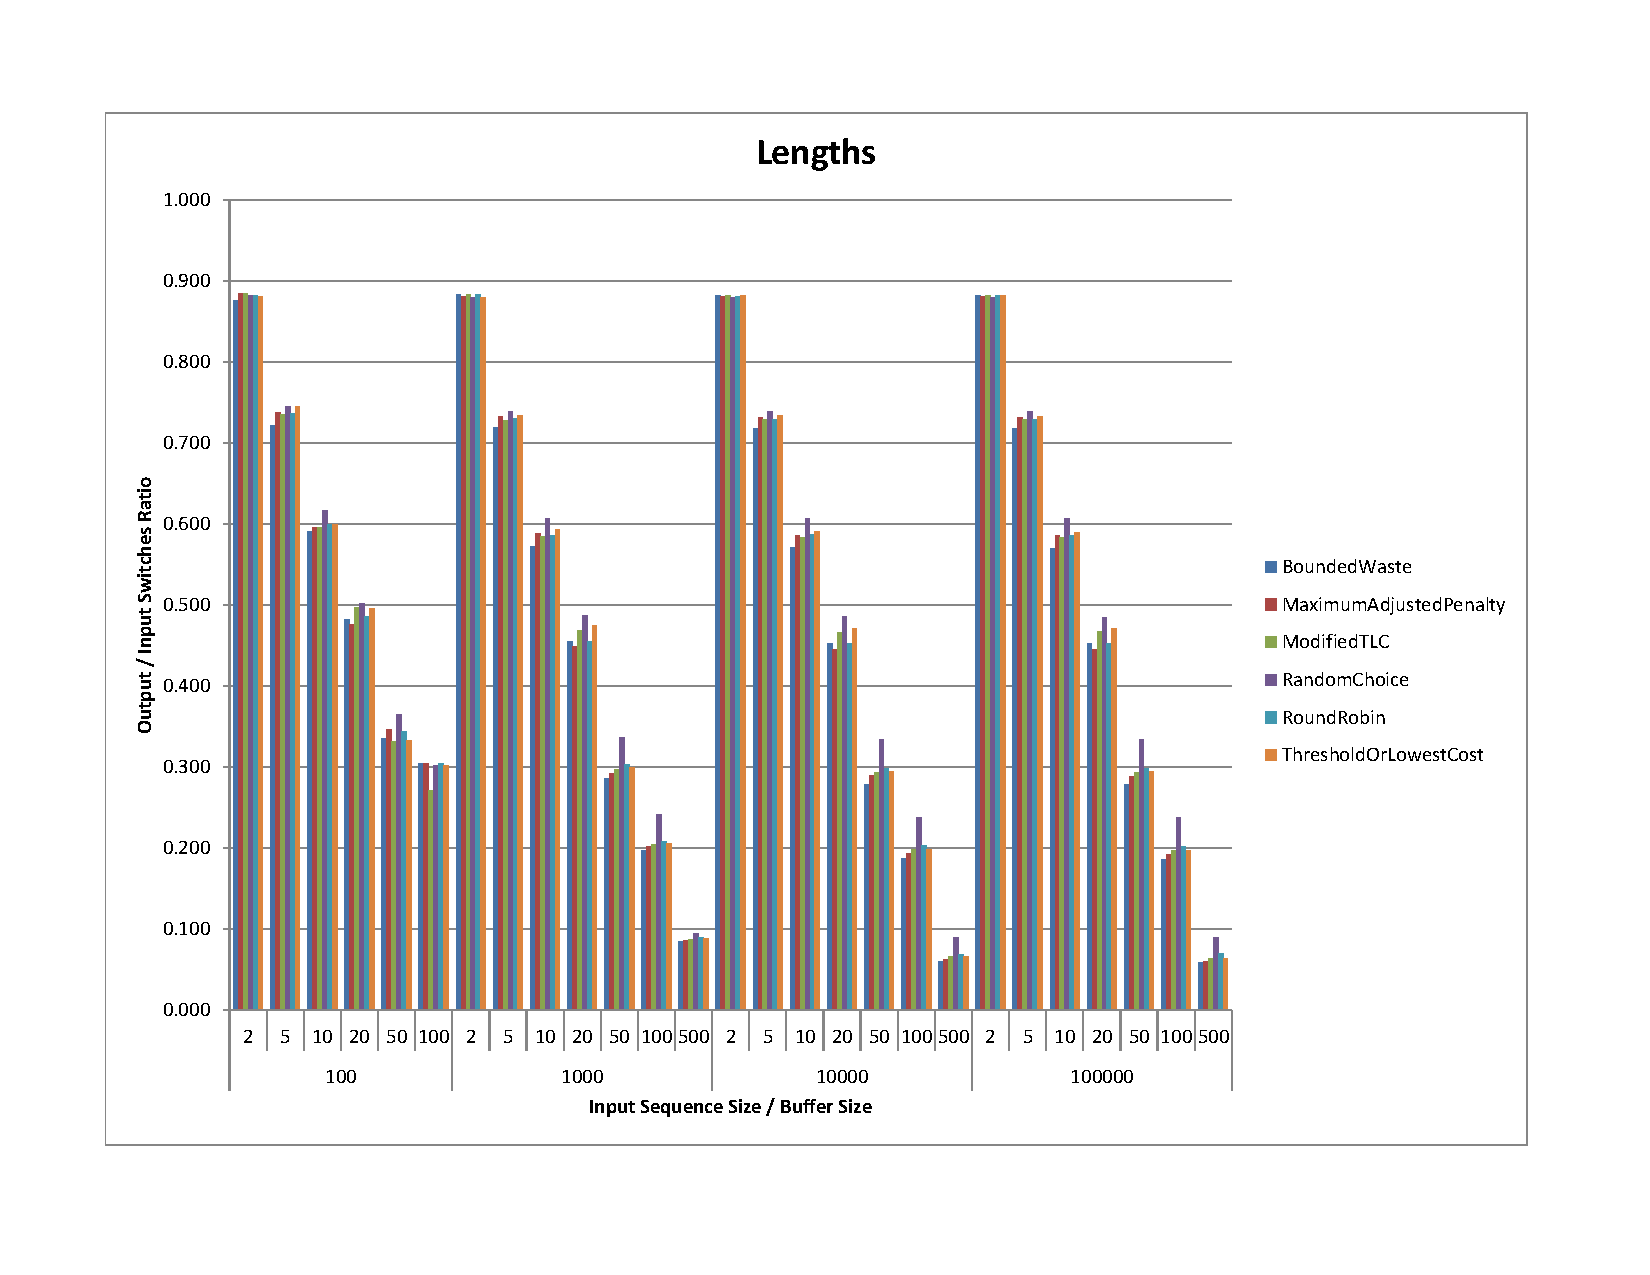
\includegraphics[scale=0.60]{Lengths.pdf}
\caption{Input Sequence Size does not impact the performance of algorithms}
\label{lengthsImpact}
\end{figure}

While different algorithms have different performance for different combinations of data sets and cost functions, the general trend suggests that they do not heavily depend on the size of the input sequence. This has been true in the case of all kinds of data sets when subjected to all different cost functions as well. 

We describe how different algorithms (with uniform and non-uniform costs) perform with the different data sets and cost function combinations in the following subsections and supplement them with appropriate figures.


\subsection{Uniform Cost}

In this section we present the performance of different uniform cost algorithms across different input sequence types and cost functions.  In the case of uniform cost algorithms, the number of switches and the cost incurred by the algorithm are the same since the exact same cost is incurred when we switch from one colour to the next. For our experiments, the uniform cost incurred on each colour switch is equal to the buffer size ($k$).

\subsubsection{Alternation Sequences}

In the case of Alternation Sequences, we observe that Bounded Waste (BW) achieves the best performance among all algorithms for larger buffer sizes. Random Choice (RC) achieves the lowest reordering while Round Robin (RR) achieves a reordering ration comparable to BW for large buffer sizes. 

For very small buffer sizes, we observe that all the algorithms fail to achieve any significant reordering with the Output/Input Switch ratio being close to 1.0 in these cases. These results are illustrated in Fig. \ref{alternationUniformBW}.

\begin{figure}[ht]
\centering 
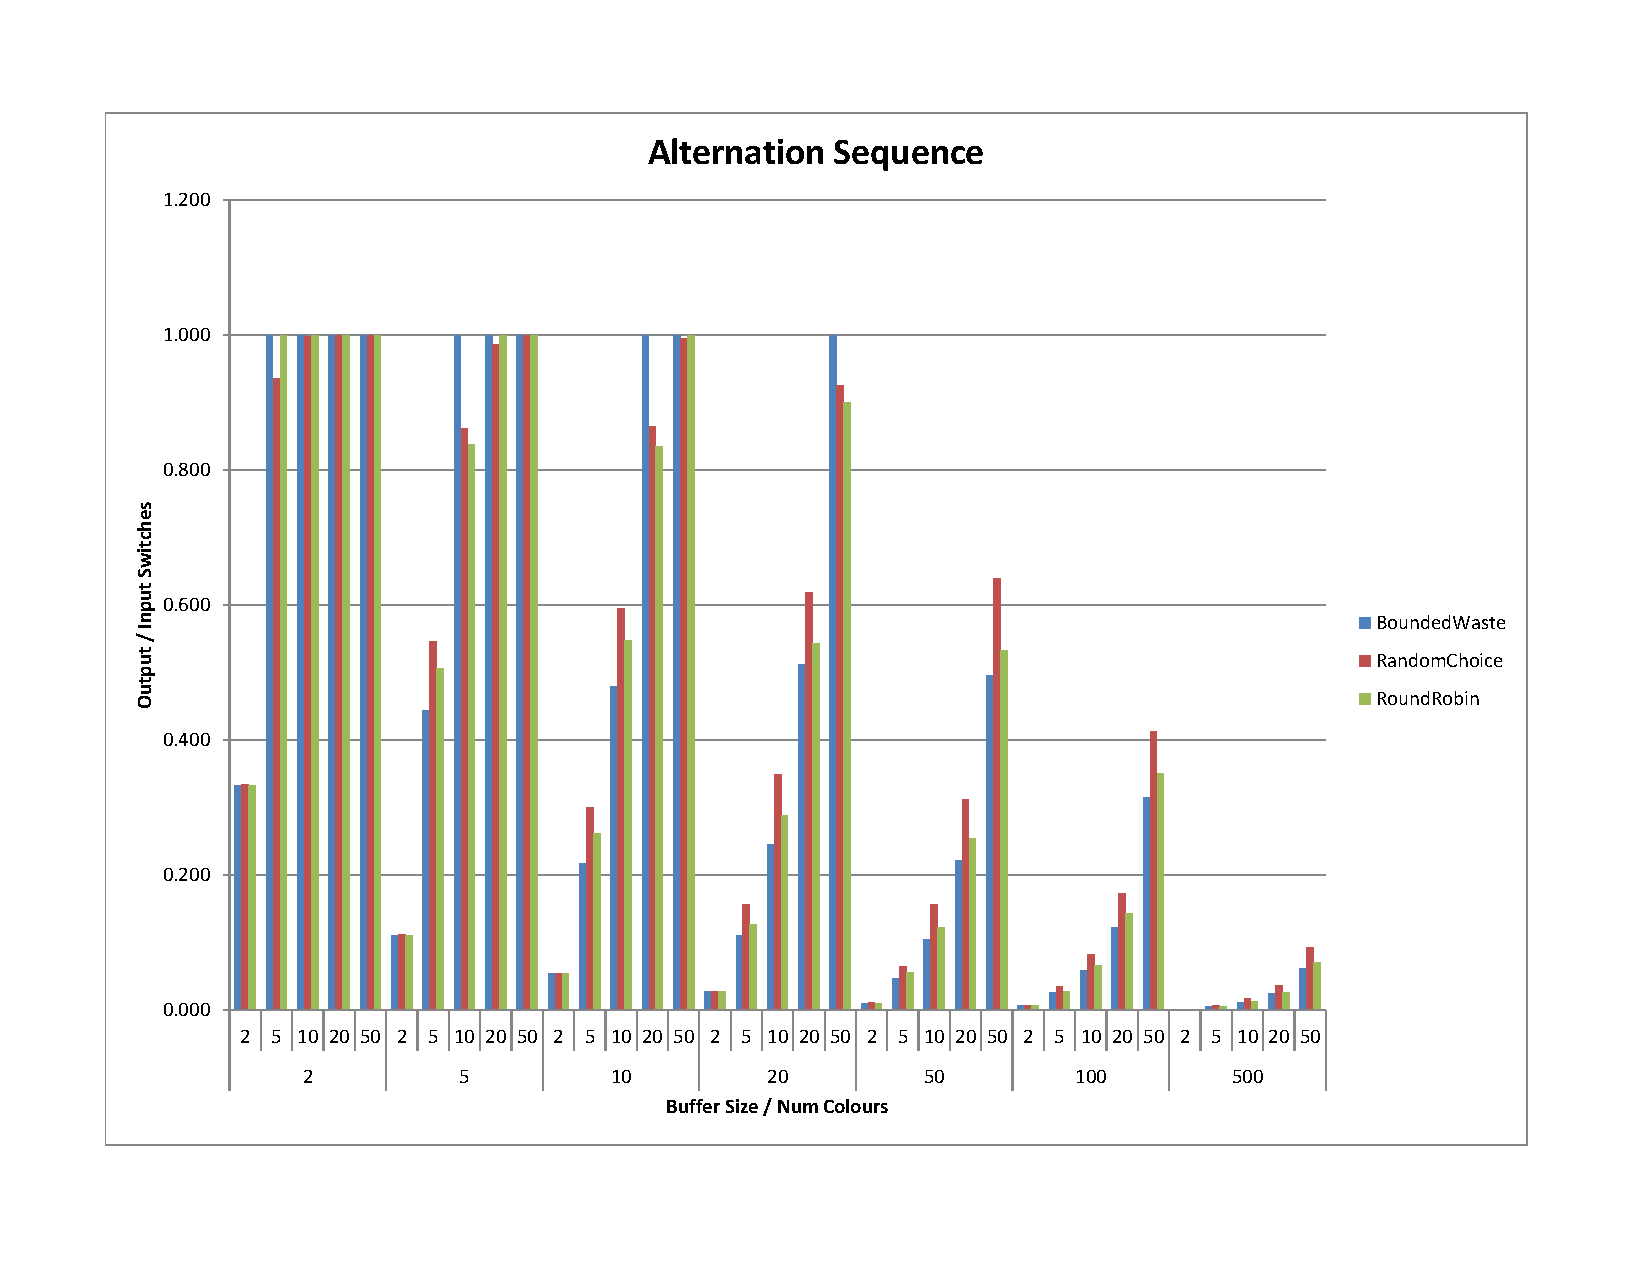
\includegraphics[scale=0.60]{Alternation-Uniform.pdf}
\caption{Bounded Waste achieves better performance}
\label{alternationUniformBW}
\end{figure}

\subsubsection{Delta Sequences}

In general, we observe that Delta Sequences achieve a better reordering ratio than Alternation Sequences across all algorithms. The reordering ratio decreases as the buffer size increases. 

We observe that all algorithms, BW, RC and RR achieve comparable performance for Delta Sequences with BW doing marginally better than the other two algorithms across all buffer size and number of colours combinations. As in the case of Alternation Sequences, RR achieves marginally better performance than RC making it the next choice after BW. These results are illustrated in Fig. \ref{deltaUniform}

\begin{figure}[ht]
\centering 
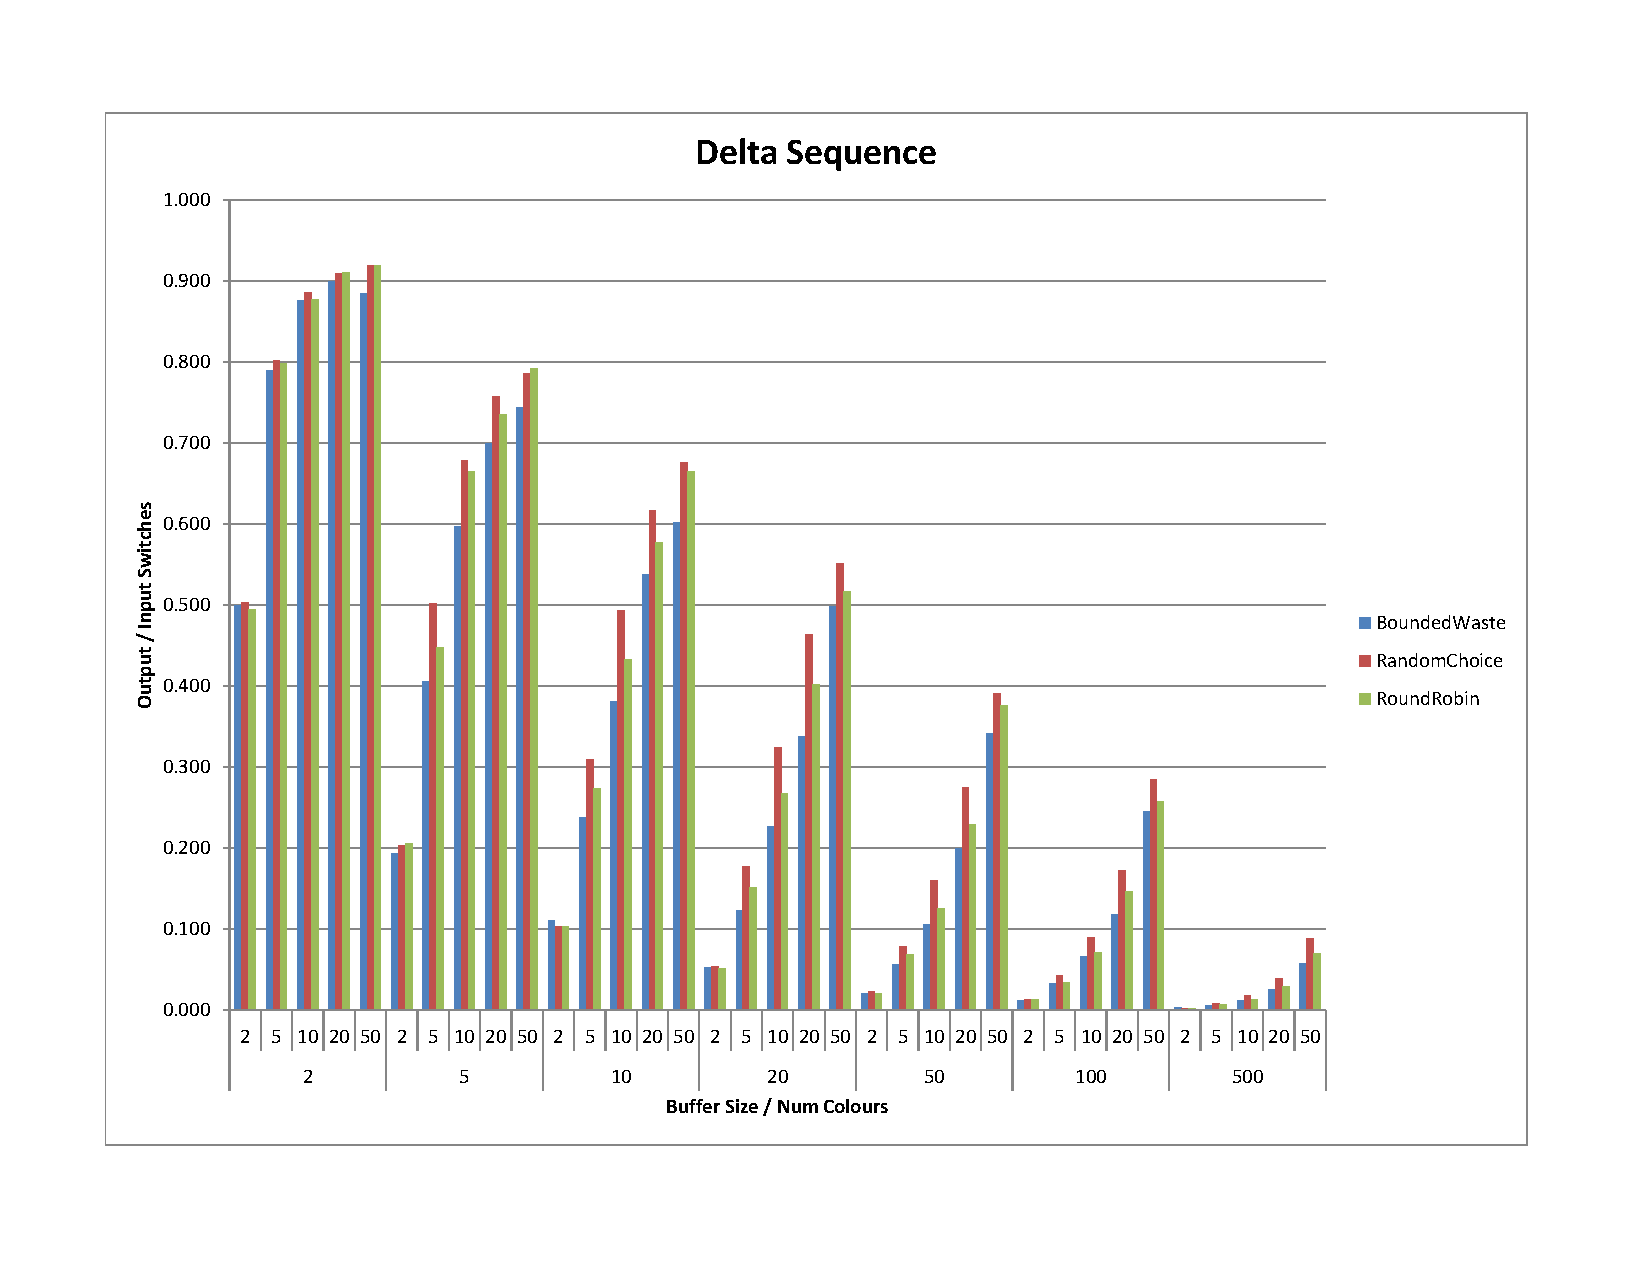
\includegraphics[scale=0.60]{Delta-Uniform.pdf}
\caption{All algorithms achieve comparable performance}
\label{deltaUniform}
\end{figure}

\subsubsection{Random Sequences}

We observe a similar trend as in the case of Delta Sequences across all buffer sizes and cost functions. As in the case of Delta Sequences, BW achieves a slightly better performance than RR and RC, however RR and RC achieve comparable reordering ratios with RR achieving a marginally better performance than RC. These results are illustrated in Fig. \ref{randomUniform}.

\begin{figure}[ht]
\centering 
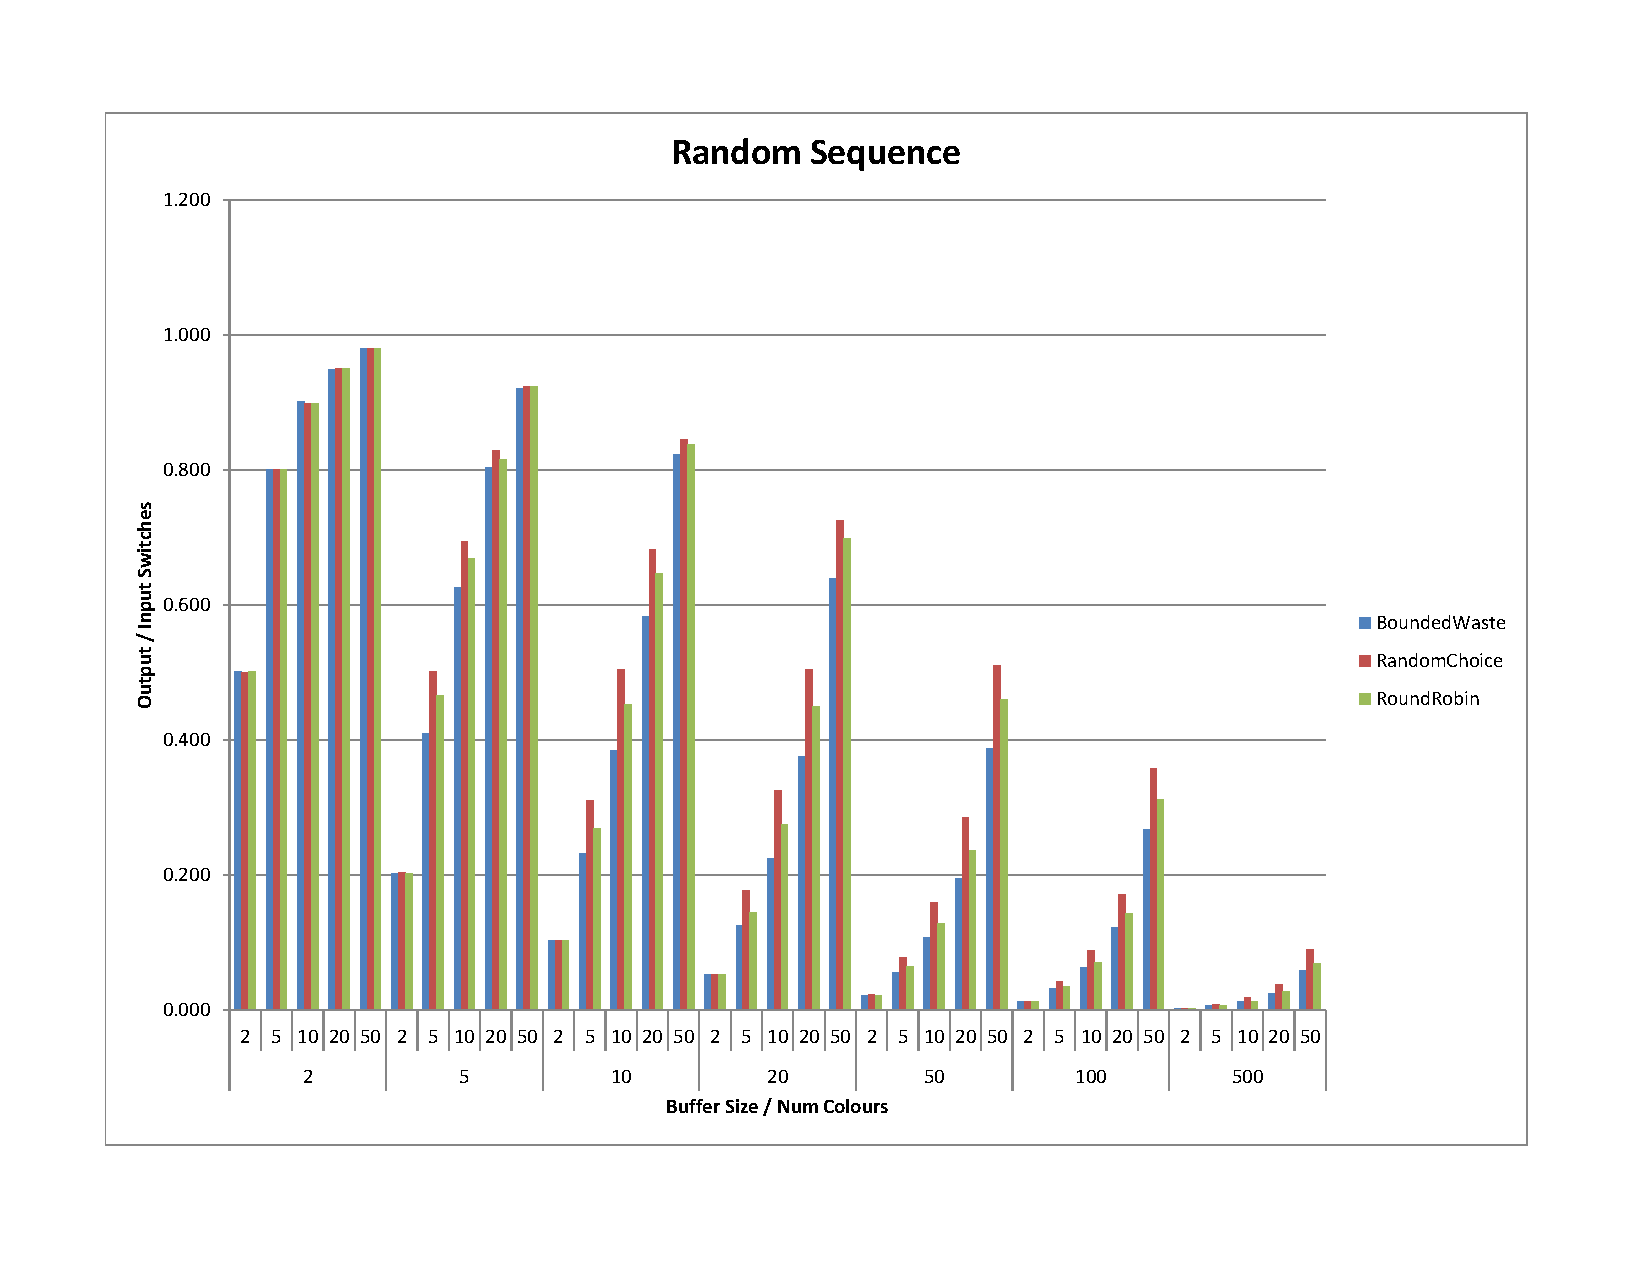
\includegraphics[scale=0.60]{Random-Uniform.pdf}
\caption{BW achieves better performance, RC and RR are comparable}
\label{randomUniform}
\end{figure}

\subsubsection{Random Block Sequences}

As expected with block sequences, all our algorithms fail to achieve a good reordering ratio as the number of colours increases, hence the reordering ratio for all our algorithms is closer to 1.0 as the number of colours increases. 

For small number of colours and large buffer sizes, BW achieves a good performance followed by RR and then RC, as is the case with other input sequences as well. These results are illustrated in Fig. \ref{randomBlockUniform}. 

\begin{figure}[ht]
\centering 
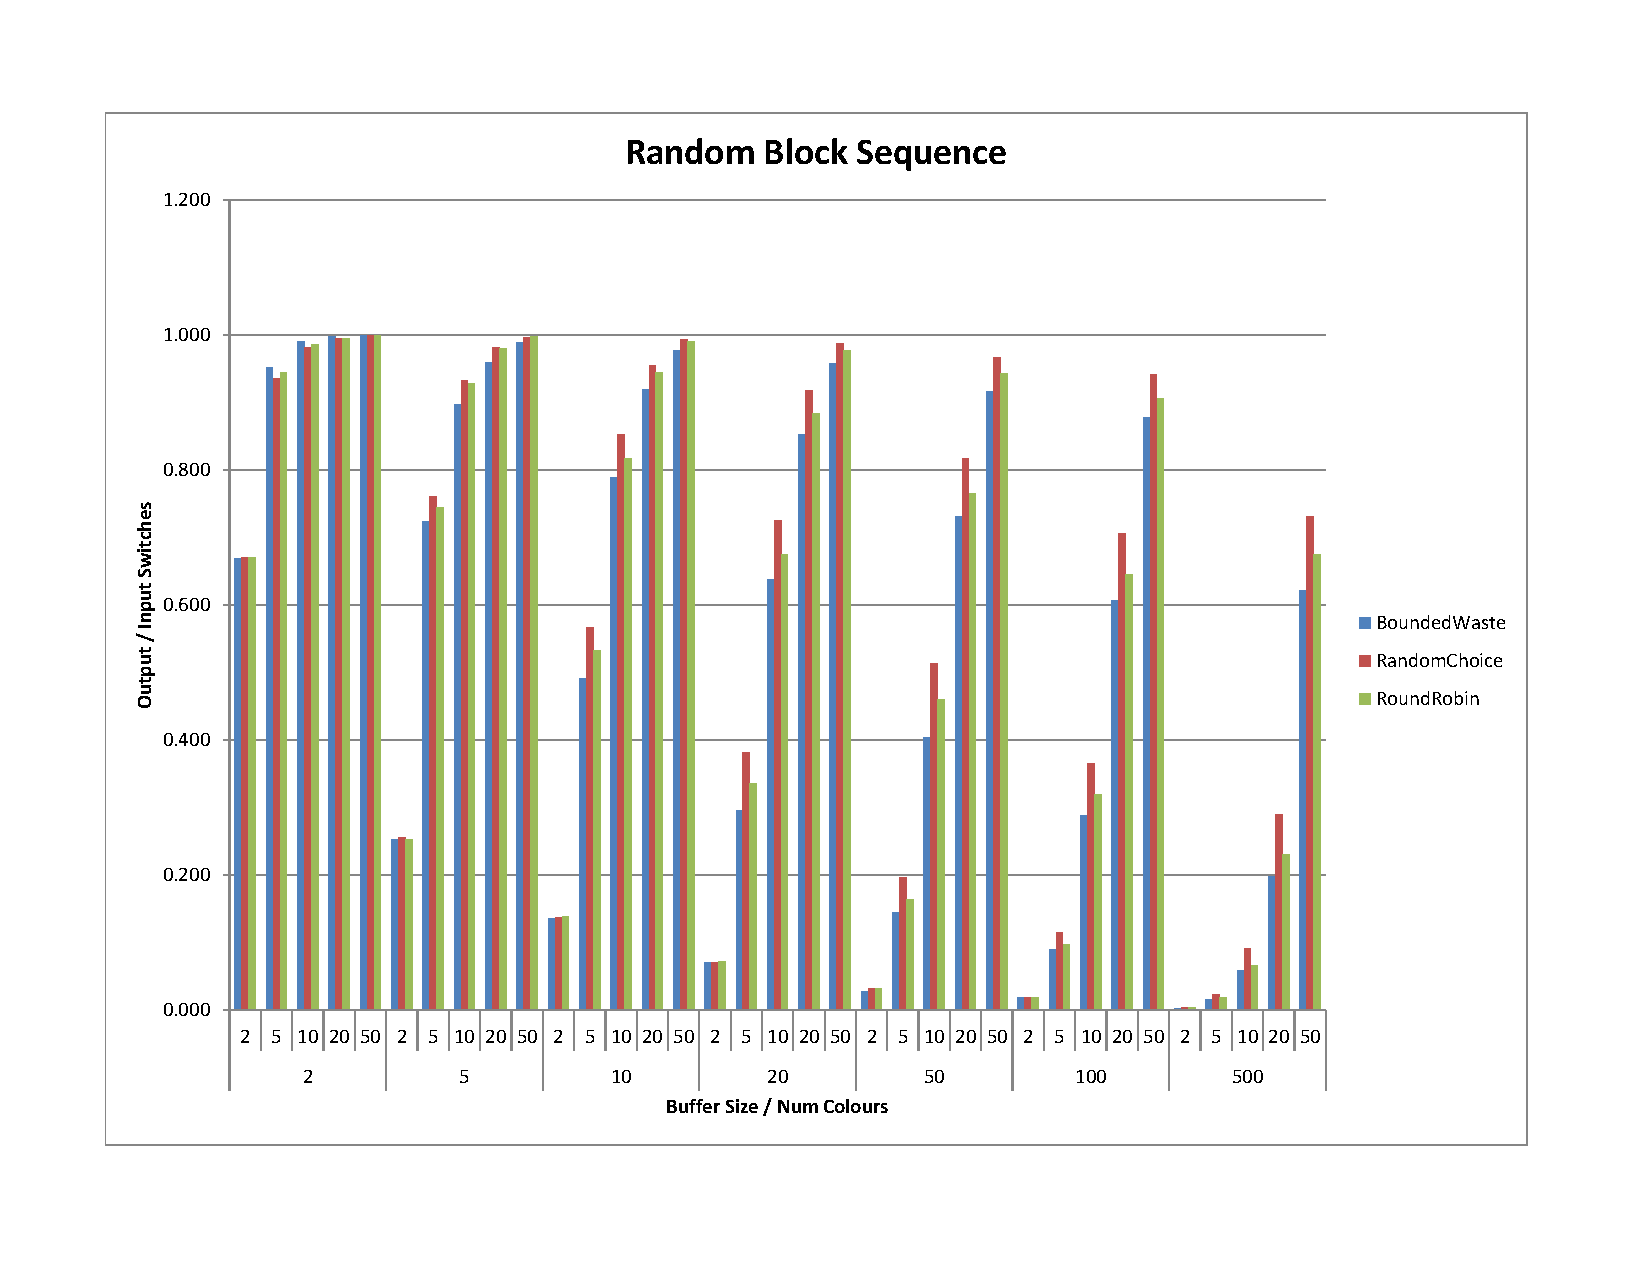
\includegraphics[scale=0.60]{Random-Block-Uniform.pdf}
\caption{Reordering Ratio is small for large number of colours}
\label{randomBlockUniform}
\end{figure}

\subsubsection{Sequential Block Sequences}

Since our block sizes are 5, we see no reordering for very small buffer sizes of 2 and 5. This is expected since only items of a single colour fill the buffer making reordering impossible for extremely small buffer sizes. 

Unlike other input sequences, BW fails to achieve the best performance across some buffer sizes making it unsuitable for application scenarios where the input items come in fixed sized blocks. While RR and RC do achieve some reordering, BW fails to reorder the input sequence making it unsuitable in these cases. 

For large buffer sizes, all our algorithms achieve comparable performance and in these cases, BW does marginally better than RR and RC. These results are illustrated in Fig. \ref{sequentialBlockUniform}.

\begin{figure}[ht]
\centering 
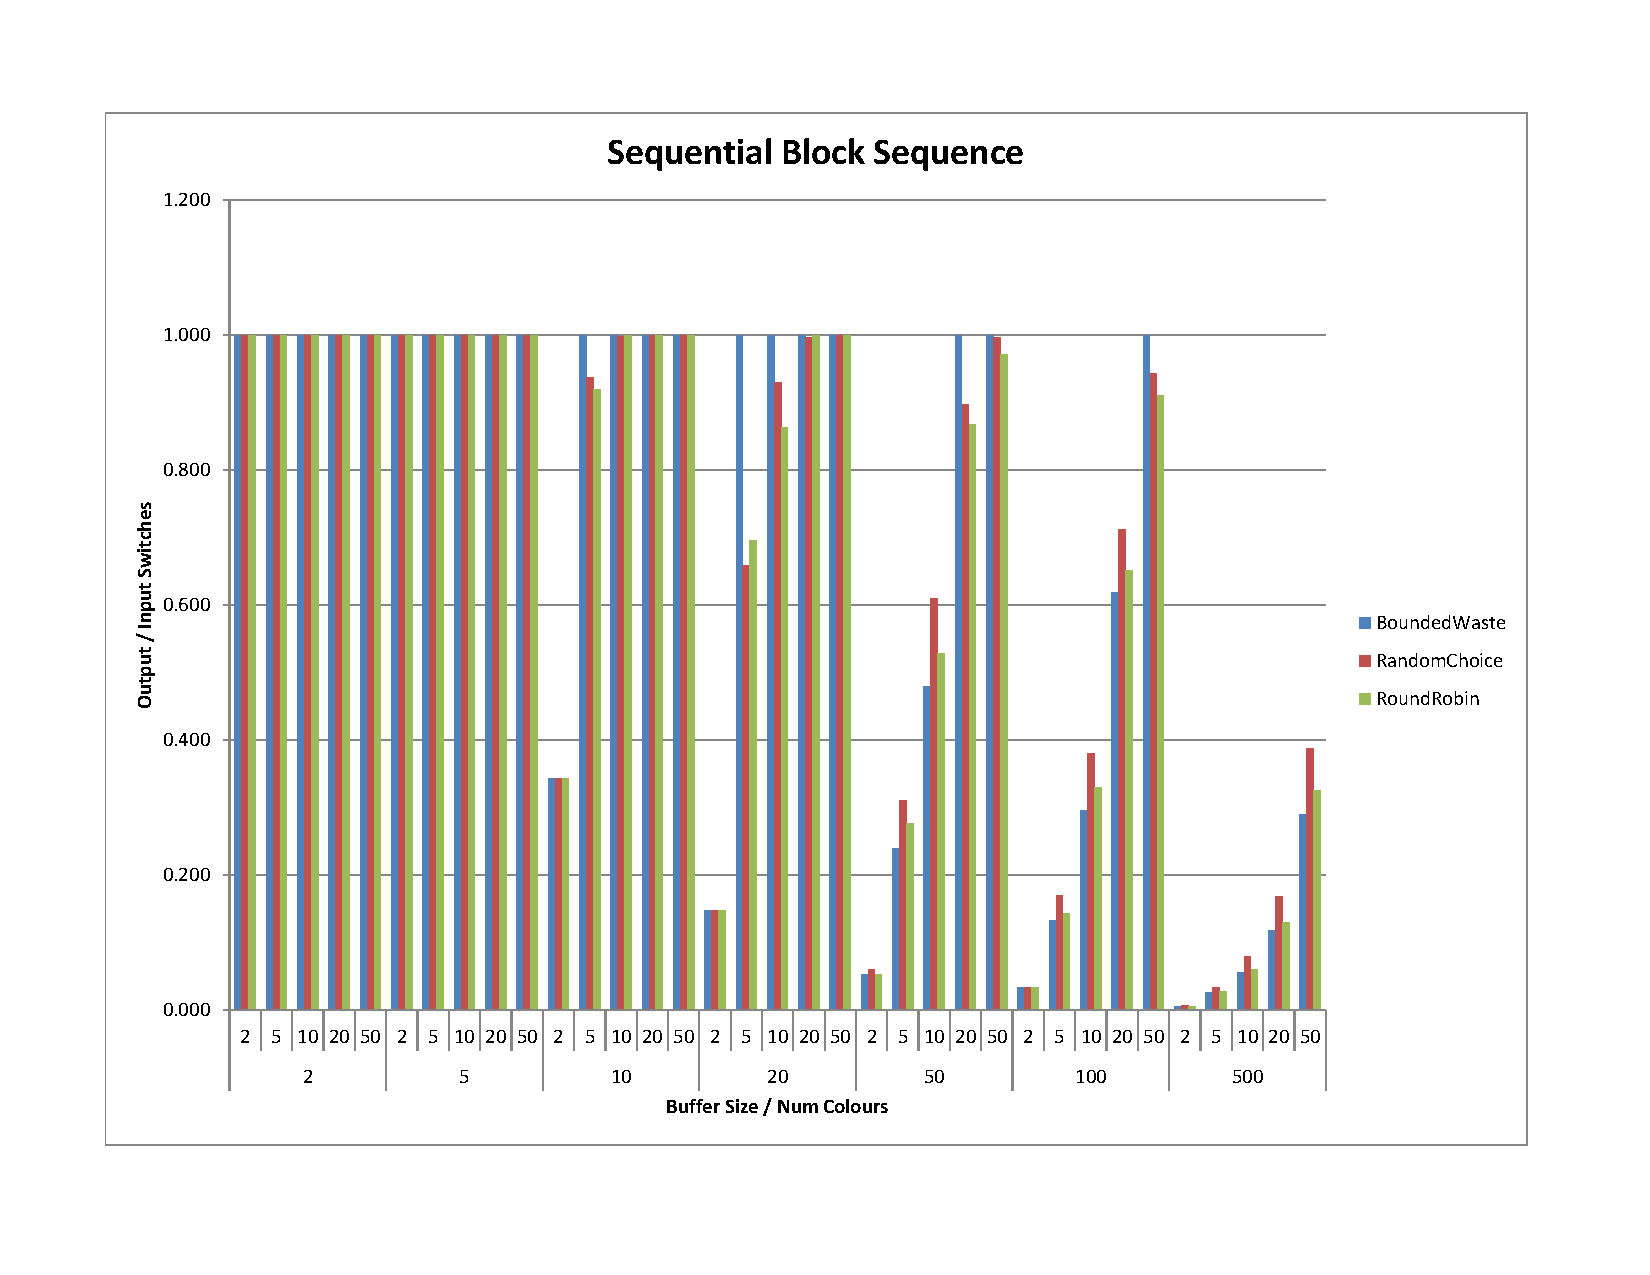
\includegraphics[scale=0.60]{Sequential-Block-Uniform.pdf}
\caption{Variation in the reordering ratios across different buffer sizes}
\label{sequentialBlockUniform}
\end{figure}

\subsection{Non-Uniform Cost}

\subsubsection{Alternation Sequences}

For Alternation Sequences with the Cost Equals Colour Cost Function, we see little or no reordering for very small buffer sizes (2 and 5). We observe that TLC achieves a better reordering switch ratio than MAP and TLC' when the number of colours is approximately two times the buffer size ($C = 2 * k$). In other cases, we observe that TLC' and MAP achieve comparable performance with TLC' slightly better than MAP. When comparing cost ratios, MAP and TLC' fail to achieve a good cost ratio for small buffer sizes, TLC' performs marginally better than MAP and TLC when the number of colours is lesser than or equals to the buffer size. As with switch ratio, TLC achieves a better performance when the number of colours is two times the buffer size. All out algorithms do not perform well when the number of colours are significantly larger than the buffer size. 

For the Cost Equals Colour Quadratic model, TLC' performs better than MAP and TLC when the number of colours is less than or equal to the buffer size, this is the same as the Cost Equals Colour Model, however, an exception to this case is buffer size 2 and 5 colours where TLC' achieves a better performance than MAP and TLC. TLC achieves a good performance when the number of colours is greater than or equal to two times the size of the buffer. These results are illustrated in Fig. \ref{alternationCQSmallCost}. TLC' achieves a better switch ratio than MAP or TLC when the number of colours is less than or equal to the number of colours, MAP and TLC achieve comparable performance in this case.

\begin{figure}[ht]
\centering 
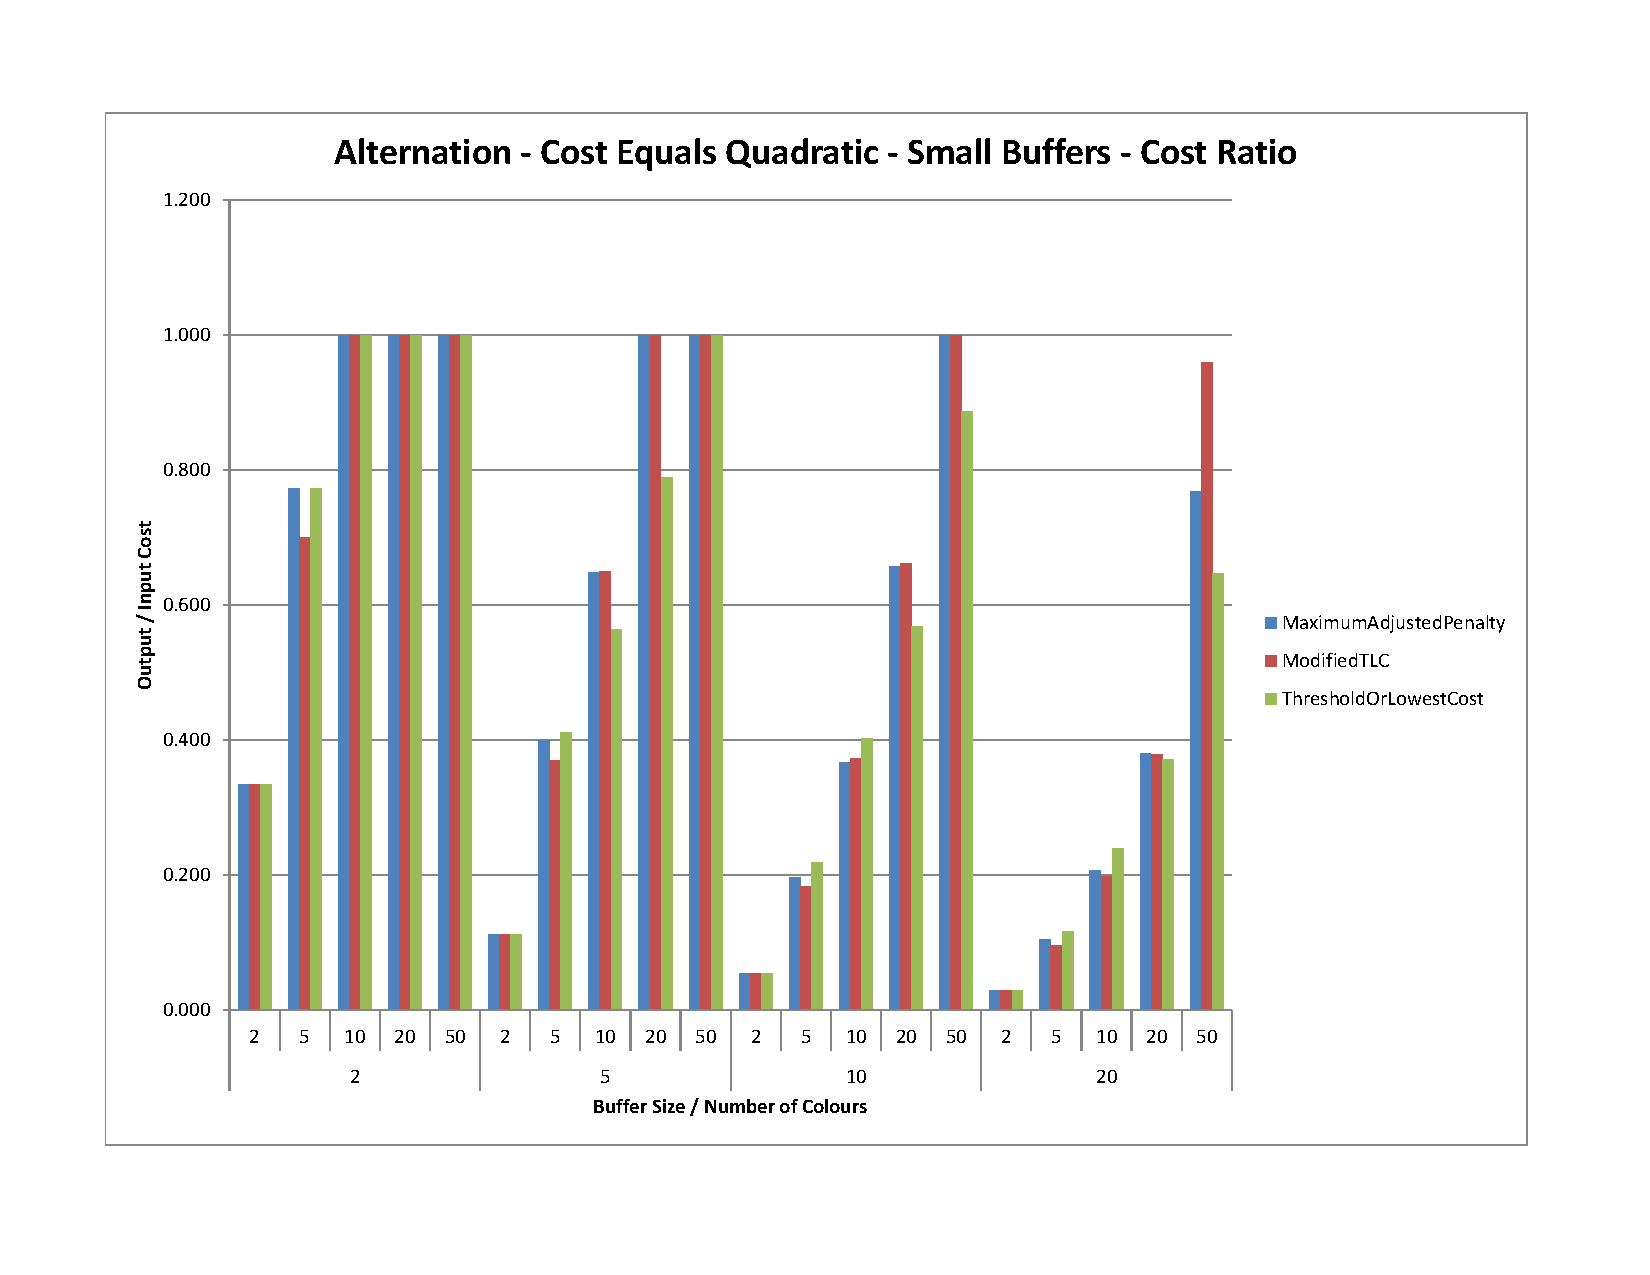
\includegraphics[scale=0.60]{Alternation-cq-small-cost.pdf}
\caption{TLC achieves a good performance when $C = 2 * k$}
\label{alternationCQSmallCost}
\end{figure} 

A similar trend is seen when comparing the algorithms against a Random Cost Function, TLC' achieves a better switch ratio than MAP and TLC when the number of colours is less than or equal to the size of the buffer. MAP achieves a better performance than TLC in this case. TLC achieves a better performance than MAP and TLC' when the number of colours is about two times the size of the buffer. MAP and TLC' have comparable performance in this case. This trend remains consistent when comparing the cost ratios with TLC achieving a better cost ratio when the number of colours is two times the size of the buffer, TLC' and MAP fail to achieve good cost ratios for small buffer sizes with TLC' having the lowest performance.  

When comparing the switches ratio for the Colour Difference cost function, TLC' achieves a better performance than MAP and TLC when the number of colours is less than or equal to the buffer size. It is interesting to note that MAP and TLC have exactly the same switch ratios for this cost function, these are slightly worse than that of TLC'. This is illustrated in Fig. \ref{alternationCDSmallSwitches}. Staying consistent with the trend, TLC' performs poorly when the number of colours is less than or equal to the buffer size for the Colour Difference cost model. However, MAP and TLC still have exactly the same cost ratios for this case as well, making them the choice of algorithm for the Colour Difference Cost Function. 

\begin{figure}[ht]
\centering 
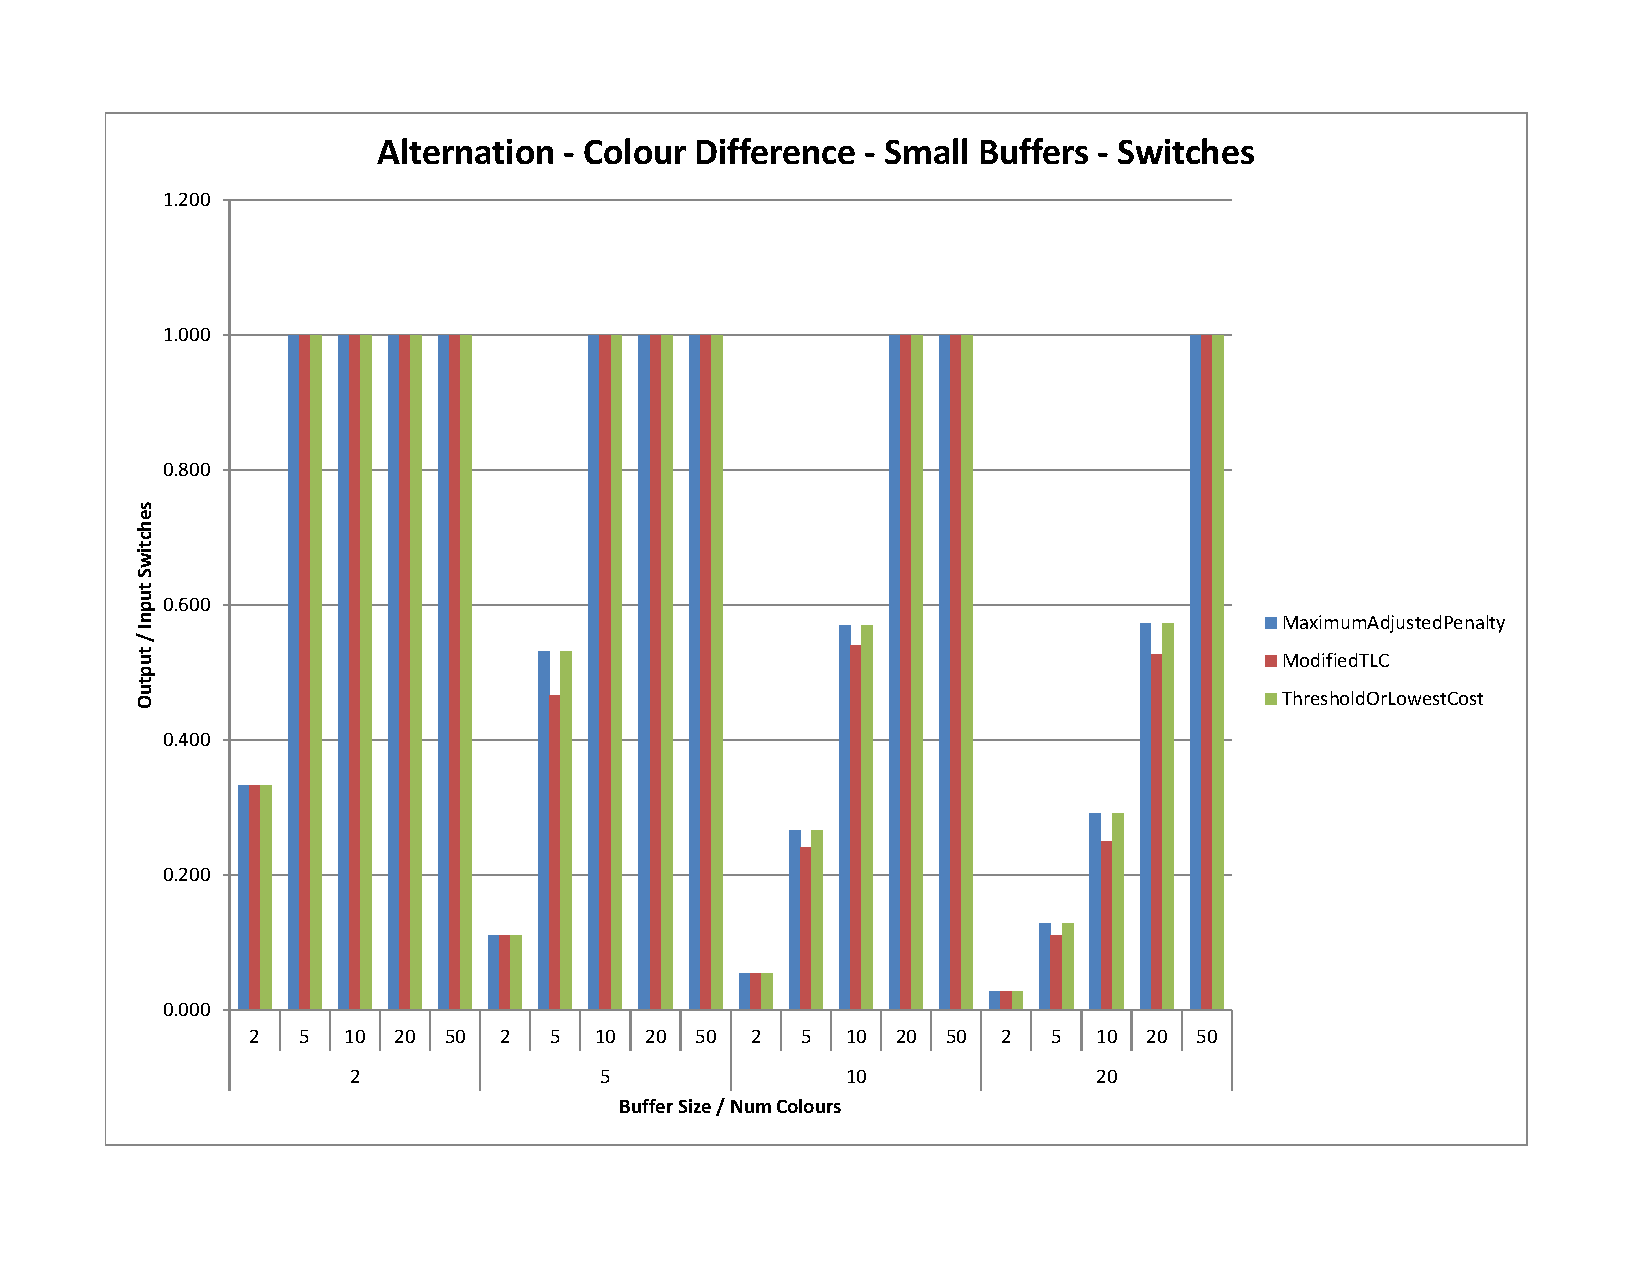
\includegraphics[scale=0.60]{Alternation-cd-small-switches.pdf}
\caption{TLC' achieves a good performance when $C <= k$}
\label{alternationCDSmallSwitches}
\end{figure} 

For medium sized buffers (50, 100 and 500), we observe that TLC' achieves a better switch ratio than TLC and MAP over all combinations of buffer sizes and number of colours. However, when comparing cost ratios, we observe that MAP and TLC' have almost identical cost ratios, where as TLC has a slightly higher cost ratio than the other two.  

We observe a similar trend with the Cost Equals Colour Quadratic cost function, where TLC' has a significantly lower switch ratio than MAP and TLC, thereby making it the choice of algorithm for this application scenario. This is illustrated in Fig. \ref{alternationCQMediumSwitches}. When comparing the cost ratios, we observe that TLC' has a higher cost ratio than MAP and TLC only for the case where the buffer size and number of colours are the same (50 and 50), for all other cases, TLC' and MAP have comparable cost ratios with TLC doing slightly worse than the other two in many cases. 

\begin{figure}[ht]
\centering 
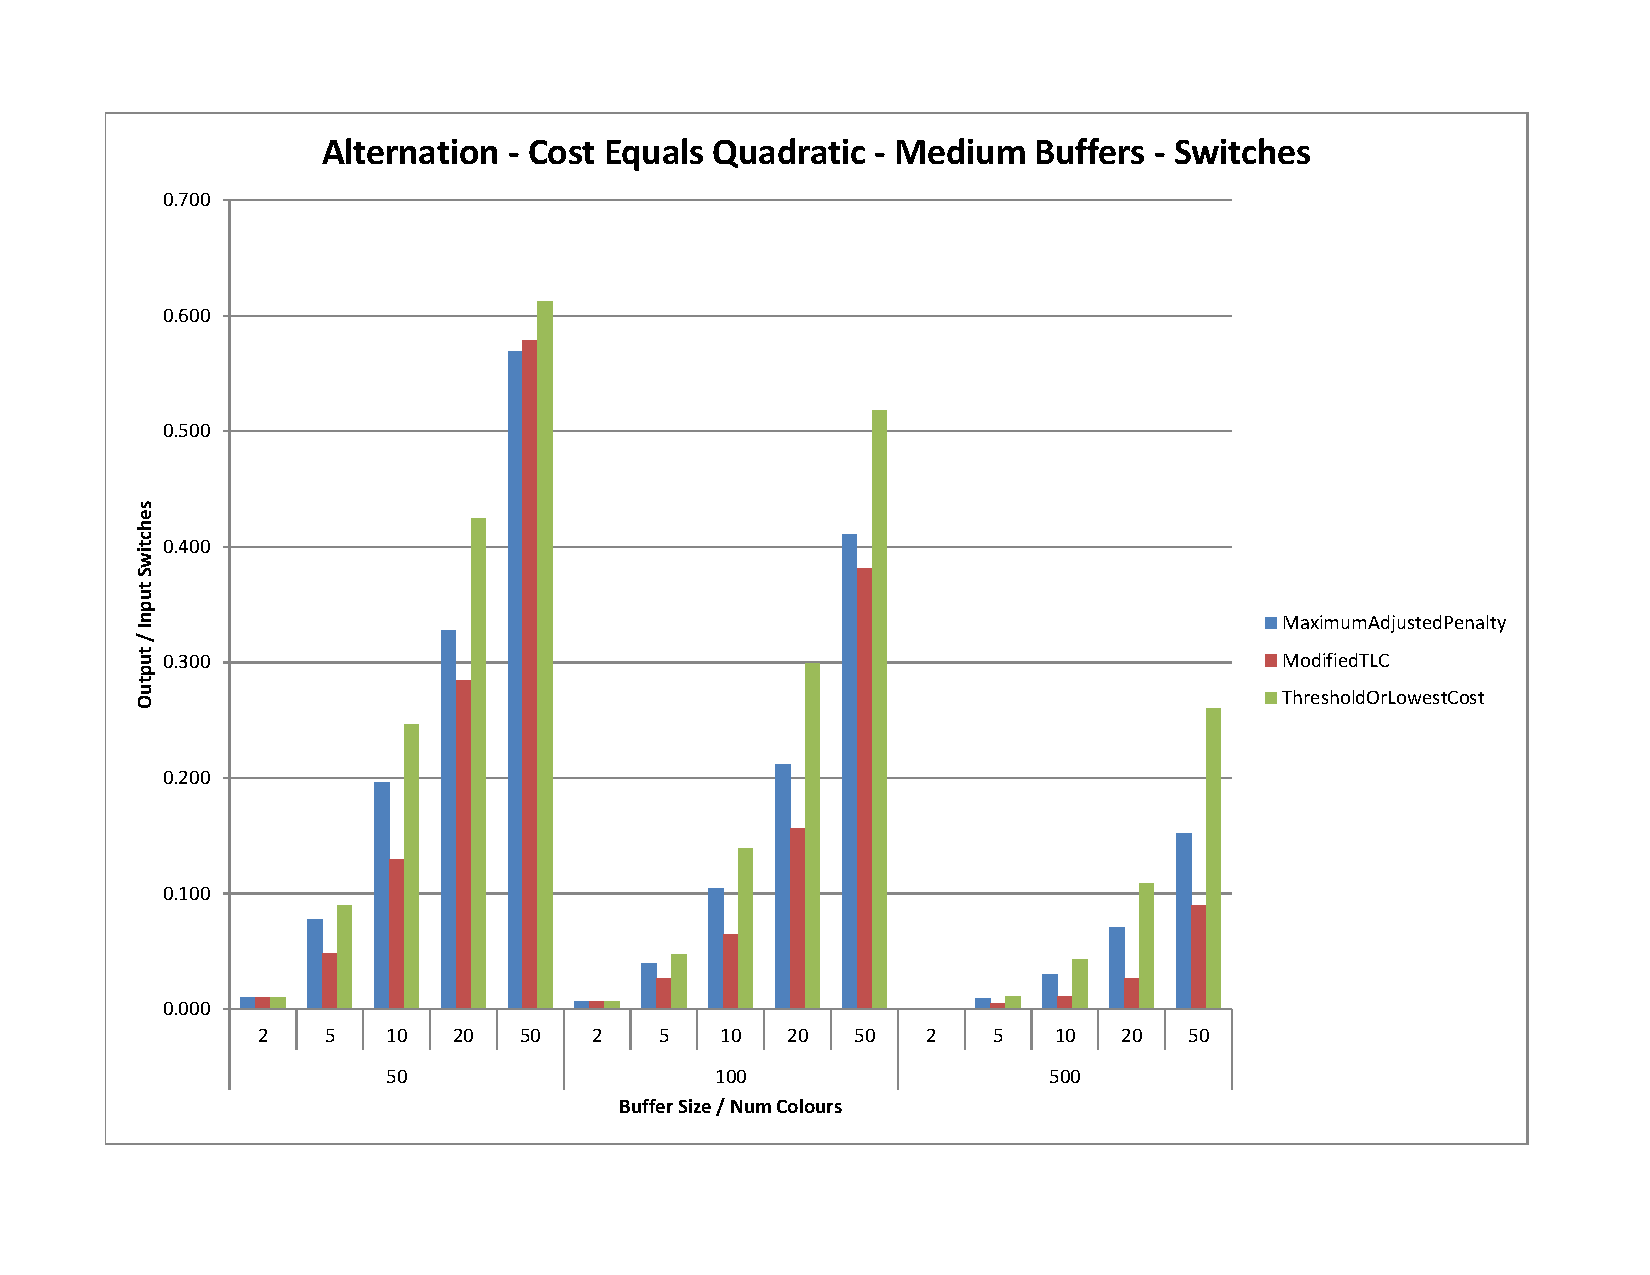
\includegraphics[scale=0.60]{Alternation-cq-medium-switches.pdf}
\caption{TLC' has significantly lower switches}
\label{alternationCQMediumSwitches}
\end{figure} 

Results observed for the Random cost function are consistent with the Cost Equals Quadratic Colour and Cost Equals Colour cost functions where TLC' has a significantly better switch ratio, we also observe the exact case where TLC' has a worse performance than TLC and MAP when the buffer size and number of colours are the same (50 ad 50). As with the other cost functions, the cost ratios for the other cases remain comparable between MAP and TLC' with TLC having a marginally worse performance. 

As observed in the case of small buffers, TLC' has a better switch ratio than TLC and MAP for the Colour Difference cost function. However, the the cost ratio for TLC' is significantly higher than that for TLC and MAP as illustrated in Fig. \ref{alternationCDMediumCost}. It is also interesting to note that TLC and MAP have exactly the same ratios when comparing both switch and cost ratios, as we see in Fig. \ref{alternationCDMediumCost}. 

\begin{figure}[ht]
\centering 
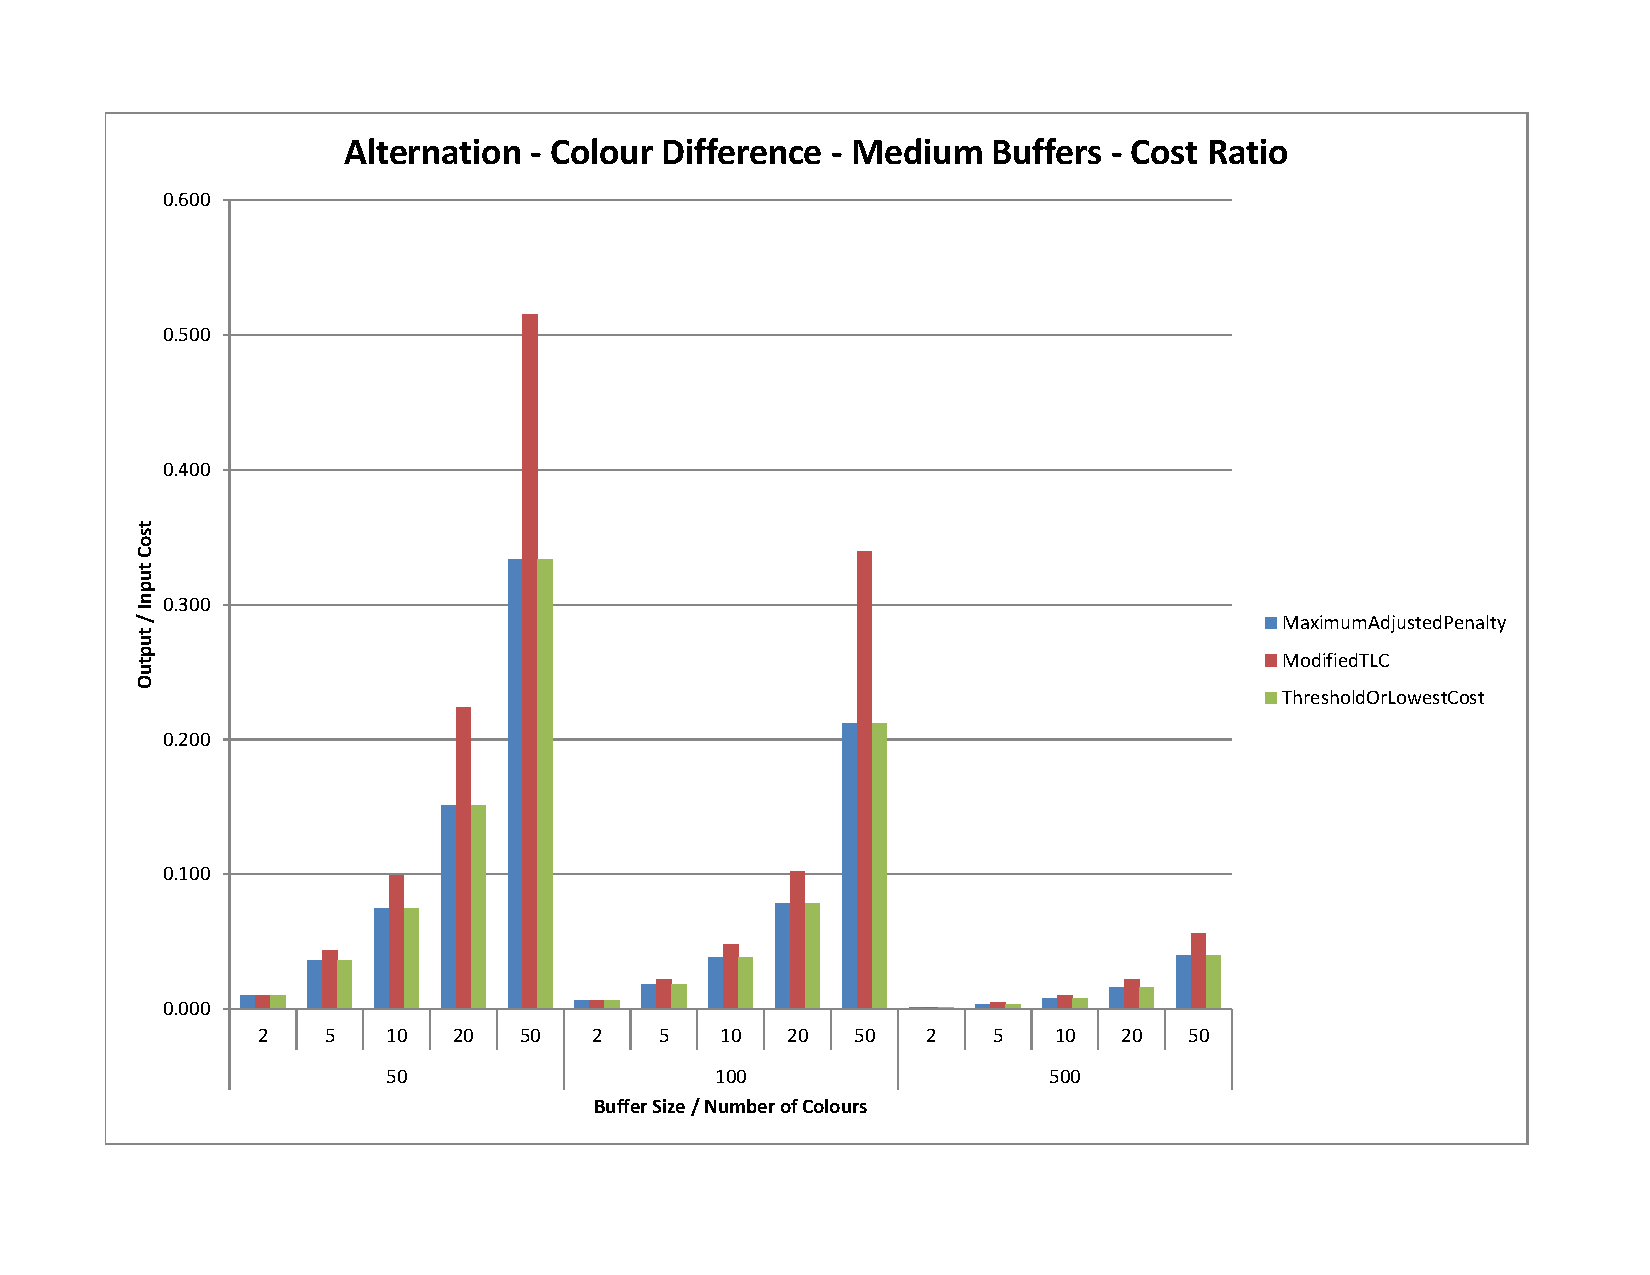
\includegraphics[scale=0.60]{Alternation-cd-medium-cost.pdf}
\caption{TLC' has significantly higher cost ratio}
\label{alternationCDMediumCost}
\end{figure} 

For the Uniform cost function, we observe that all out algorithm have almost identical switch and cost ratios, with only very marginal differences. 

\subsubsection{Delta Sequences}

When comparing the cost ratios across our algorithms for the Cost Equals Colour cost function, we observe that TLC' achieves a slightly better performance than TLC and MAP for small buffers. This is illustrated in Fig. TLC' also achieves a better switch ratio than MAP and TLC with MAP performing slightly better than TLC for small buffers.

\begin{figure}[ht]
\centering 
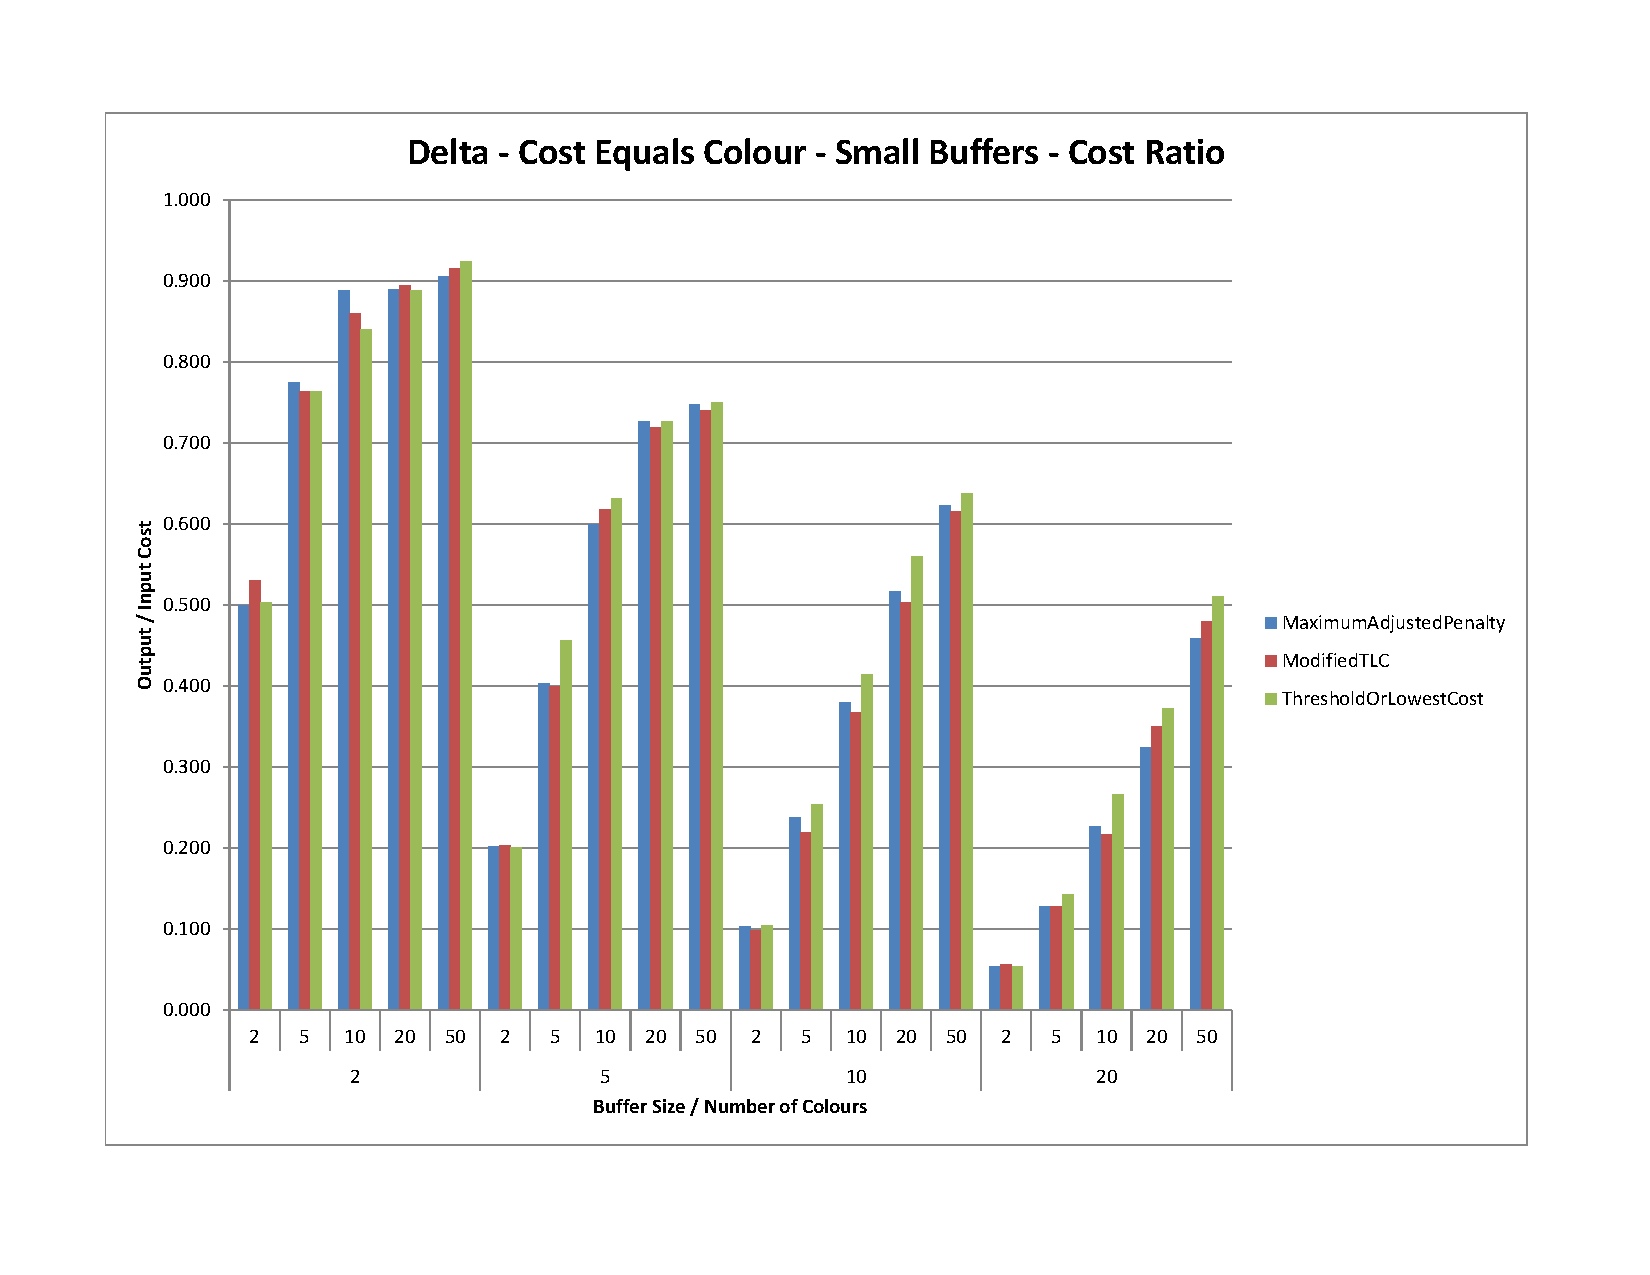
\includegraphics[scale=0.60]{Delta-cc-small-cost.pdf}
\caption{TLC' achieves a better performance than MAP and TLC}
\label{deltaCCSmallCost}
\end{figure}   

In the case of Cost Equals Colour Quadratic cost function, TLC' achieves a significantly better switch ratio than TLC and MAP across all small buffer sizes. This is illustrated in Fig. MAP performs better than TLC with TLC having the worst switch ratio for this cost model. When comparing the cost ratios, all our algorithms achieve comparable performance with TLC' and MAP having better performance than TLC; TLC' has a marginally better cost ratio than MAP in many cases. 

\begin{figure}[ht]
\centering 
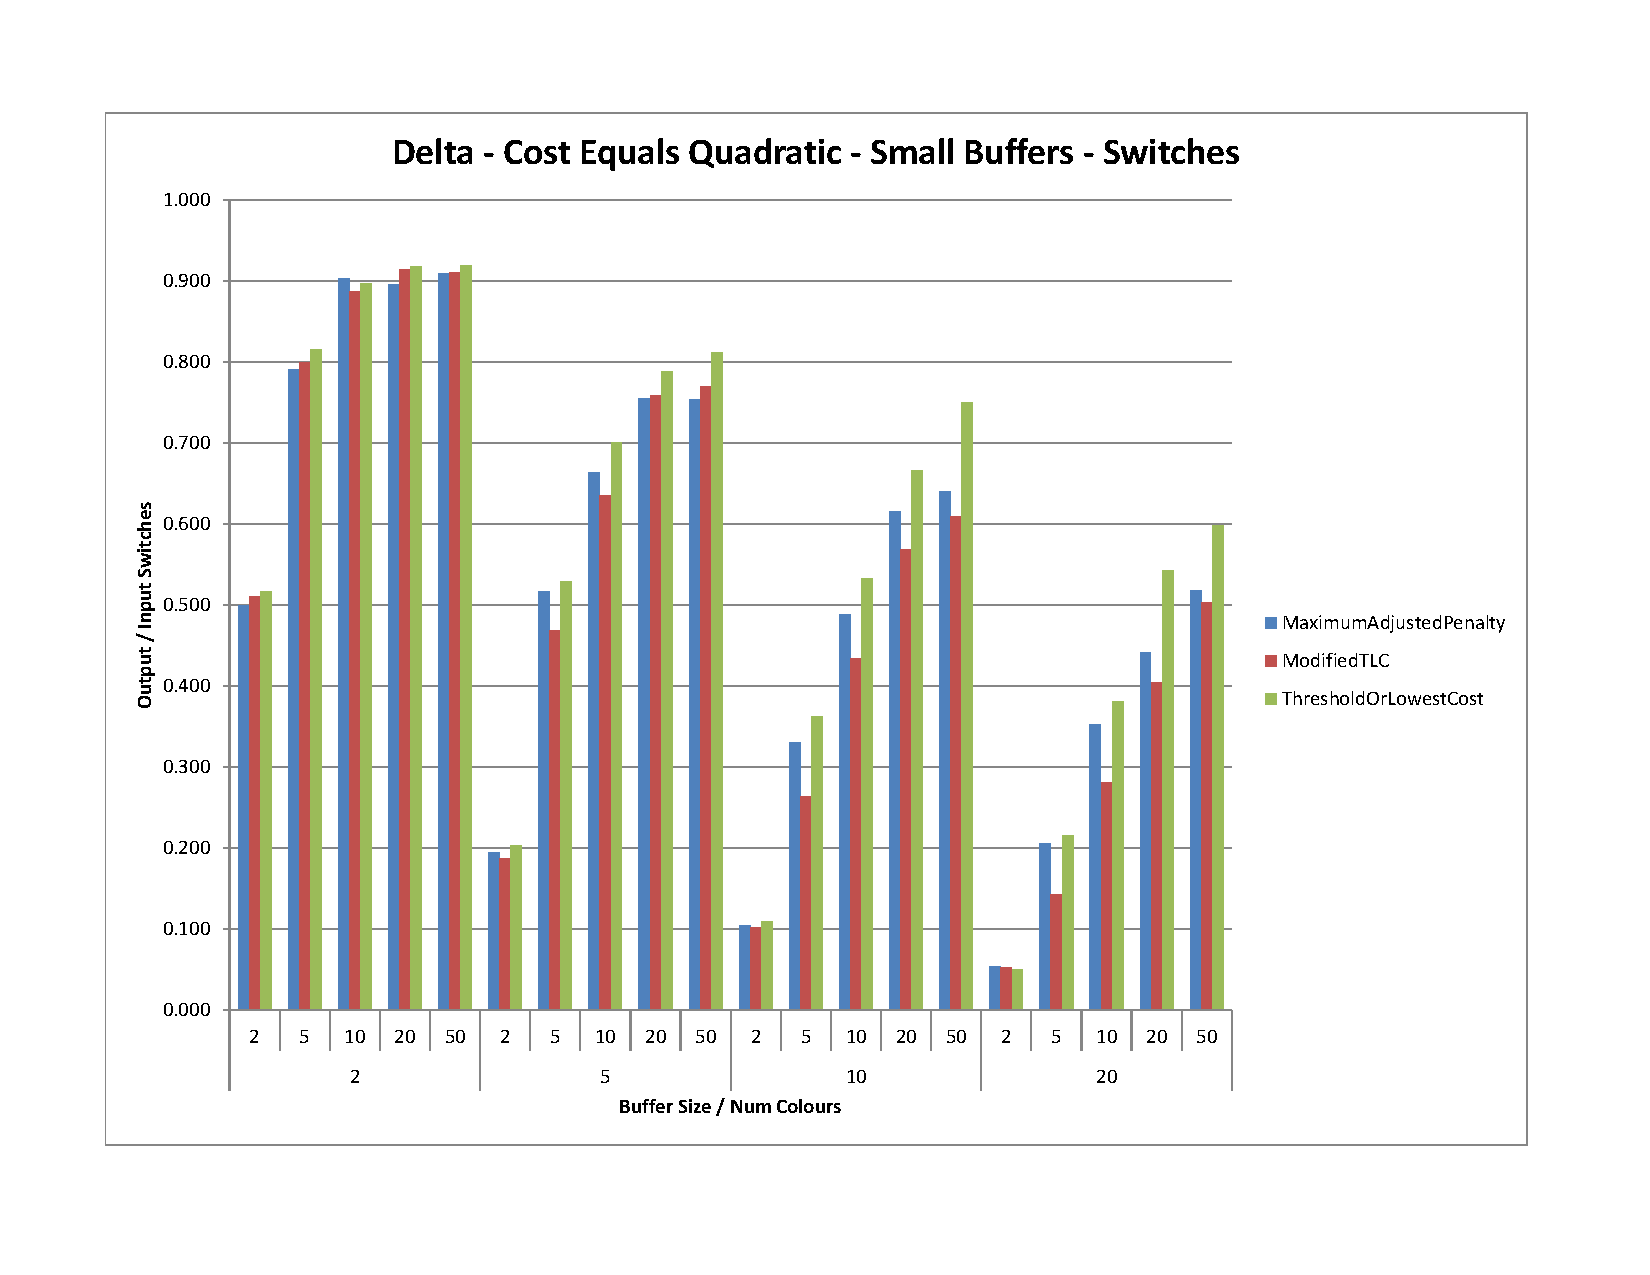
\includegraphics[scale=0.60]{Delta-cq-small-switches.pdf}
\caption{TLC' achieves a better switch ratio than MAP and TLC}
\label{deltaCQSmallSwitches}
\end{figure}   

All our algorithms achieve almost exactly the same cost ratios for the Random cost function, with TLC doing very marginally worse than the other two. However, when comparing the switch ratios for these algorithms, we observe that TLC' achieves a better switch ratio than MAP and TLC for most small buffer sizes, with buffer size 2 being an exception where all our algorithms achieve the same performance. We also observe that MAP performs better than TLC when switches are compared. 

As in the case of Alternation sequences, although TLC' has a better switch ratio than MAP and TLC we observe that like with Alternation Sequences, the cost ratio is significantly higher for TLC' when compared to TLC and MAP. TLC achieves the best performance in terms of cost ratios while MAP has a comparable performance. 

TLC has a significantly better switch ratio than MAP or TLC for medium buffers, while the cost ratio is not significantly better, TLC still has better cost ratios than TLC and MAP for all buffer sizes, except the case when $k = 50$ and $C = 50$. In this case, MAP does slightly better than TLC'. 

In the case of the Cost Equals Quadratic Colour cost function, TLC' has a better switch ratio compared to TLC and MAP across all medium sized buffers. But when we compare the cost ratios, TLC' has a slightly better cost ratio for most cases except when the buffer size is 50 and number of colour is 50, in this case MAP does slightly better than TLC and TLC'. Another exception is when the buffer size is 100 and number of colours is 50, TLC does slightly better than MAP and TLC'. 

For Random costs, we see that TLC' does better than TLC and MAP when we compare both switch and cost ratios. While the performance is significantly better when comparing switches, it is slightly better when comparing costs as illustrated in the Fig.  \ref{deltaRCMediumCost}.

\begin{figure}[ht]
\centering 
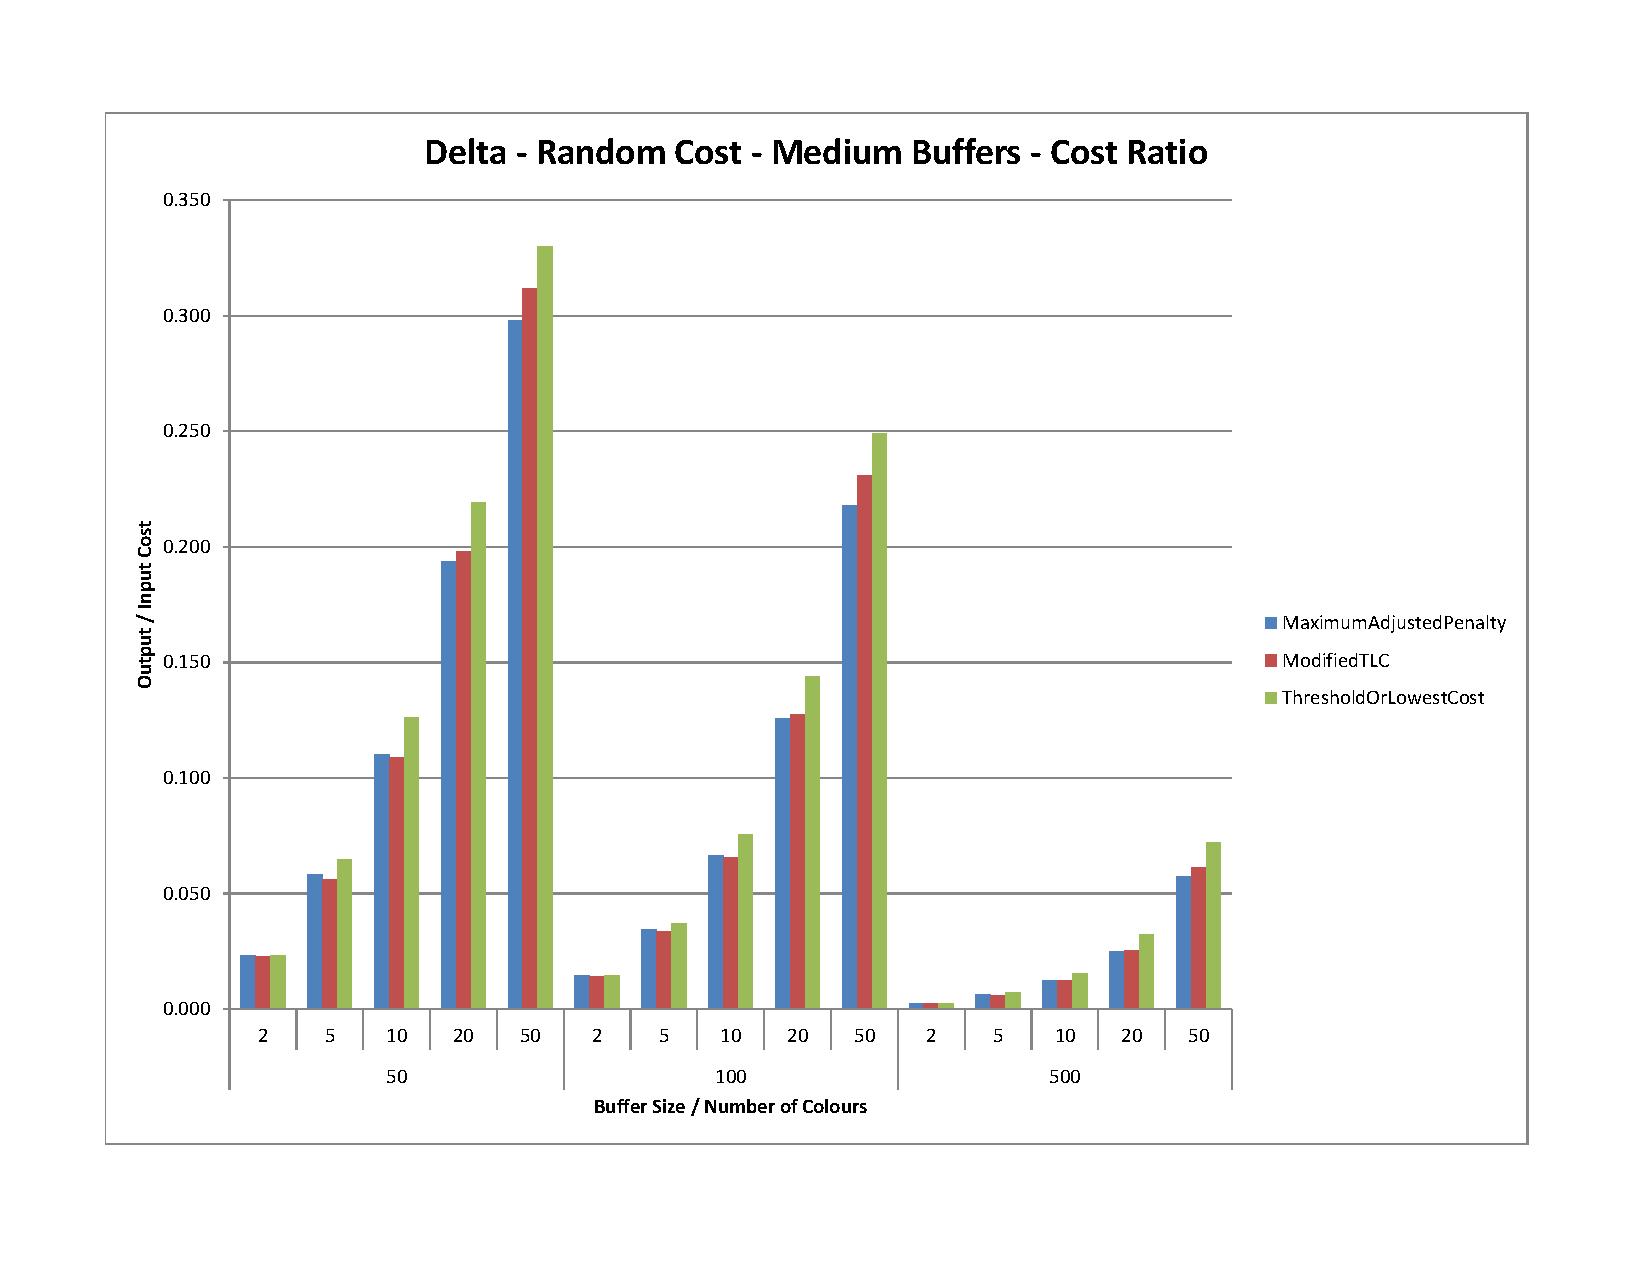
\includegraphics[scale=0.60]{Delta-rc-medium-cost.pdf}
\caption{TLC' has a lower cost ratio than MAP and TLC}
\label{deltaRCMediumCost}
\end{figure}   

We observe that TLC' has lower switch ratios than TLC and MAP for the Colour Difference cost function. While the switch ratios are lower, we also observe that the cost ratios are significantly higher than what we see for TLC and MAP, as illustrated in Fig. \ref{deltaCDMediumCost}. It is also to be noted that while the cost ratio is significantly higher it is only when compared to TLC and MAP, overall all our algorithms achieve very good cost ratios as well below 45\% indicating that more than half the cost has been eliminated. This can be inferred from Fig. \ref{deltaCDMediumCost}.

\begin{figure}[ht]
\centering 
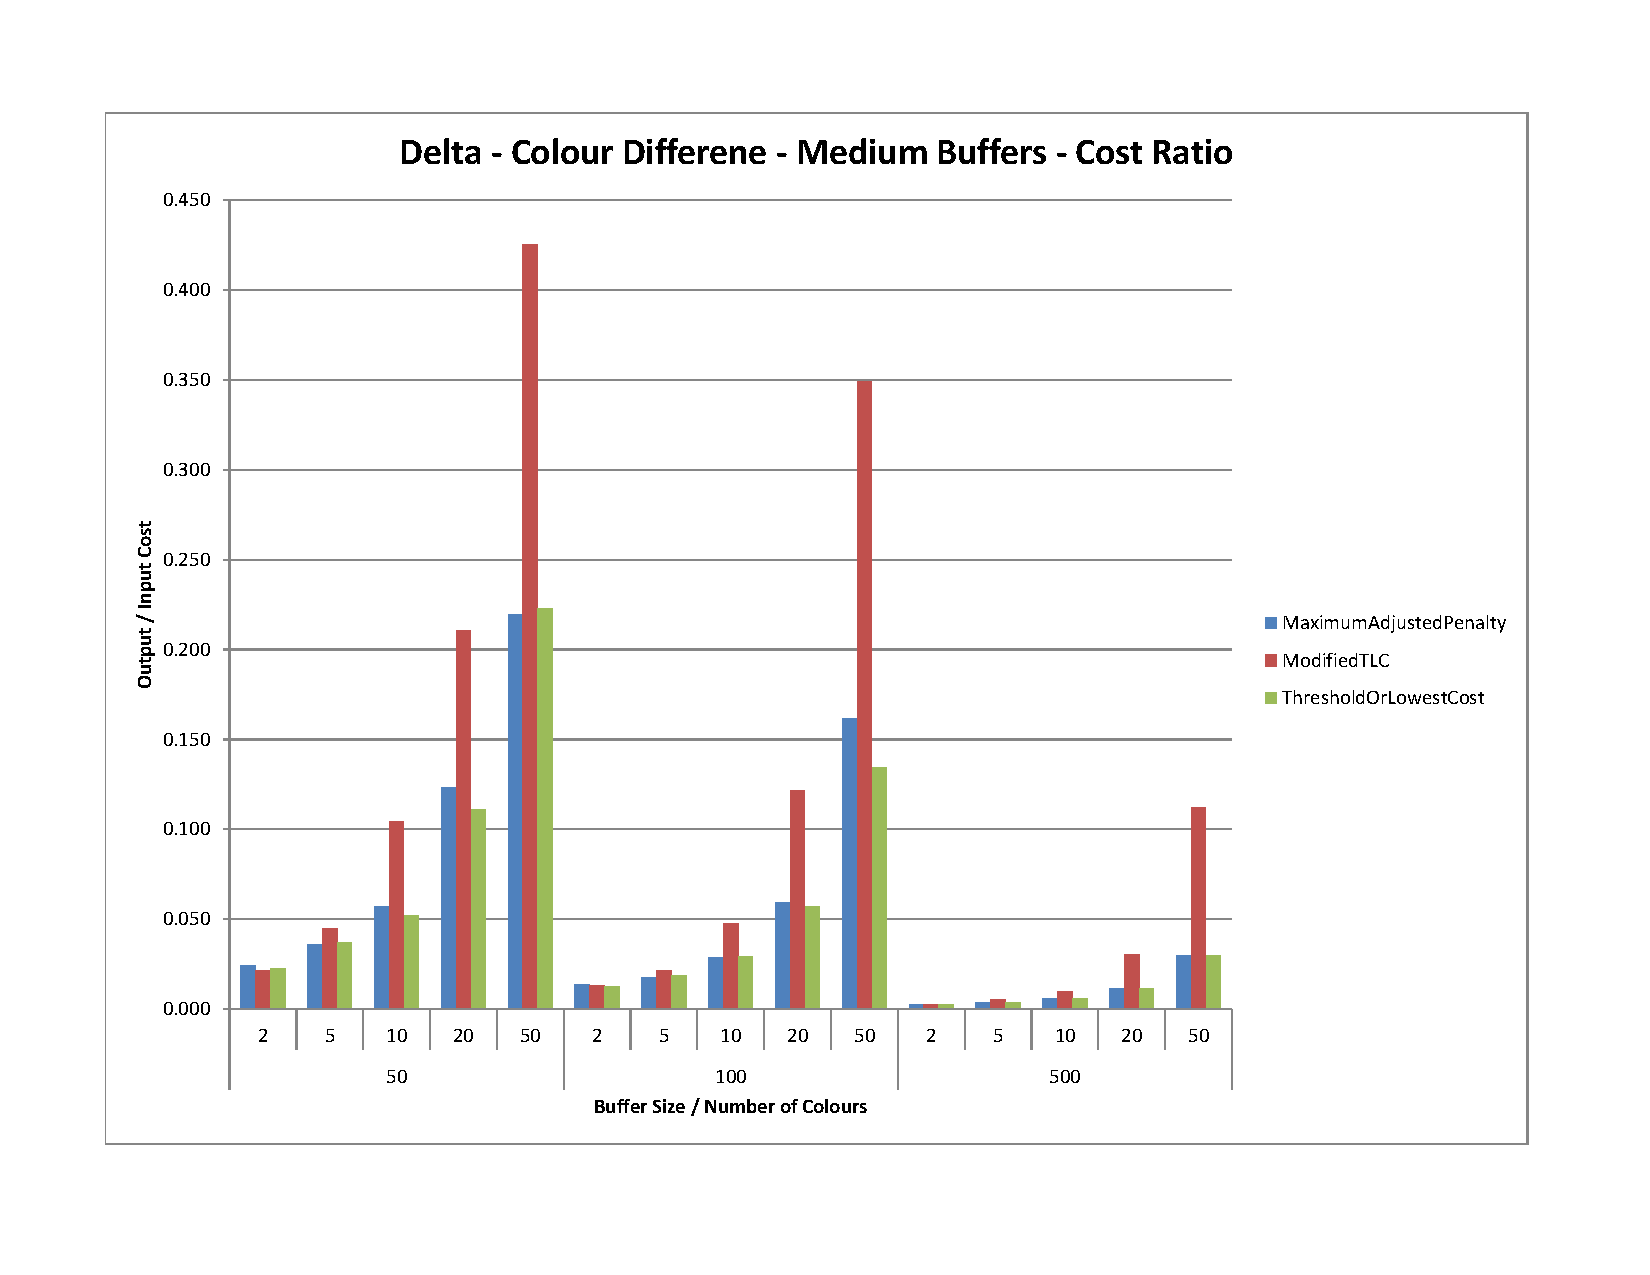
\includegraphics[scale=0.60]{Delta-cd-medium-cost.pdf}
\caption{TLC' performs poorly when comparing cost ratios with MAP and TLC}
\label{deltaCDMediumCost}
\end{figure}   

All our algorithms achieve a good performance for the Uniform cost function having almost identical cost ratios. An exception is the case when the buffer size is 50 and number of colours is 50, in this case MAP does slightly worse than the other two algorithms.

\subsubsection{Random Sequences}

For the Cost Equals Colour cost function, we observer that TLC' performs only marginally worse than TLC and MAP when comparing cost functions when the number of colours is greater than the buffer size. For other cases, it has a better cost ratio than TLC. Overall, We also observe that the cost ratios all our algorithms have comparable cost ratios with only very small variations. However, when comparing switch ratios, we observe that TLC' achieves a better switch ratio than MAP and TLC across all buffer size and number of colour combinations. 

We observe a similar trend with the Cost Equals Quadratic Colour cost function where TLC' achieves a better switch ratio than TLC and MAP across all combinations, but has a higher cost ratio compared to the other two. When comparing costs, we observe that TLC' has a higher cost ratio than TLC and MAP for all combinations where the number of colours is greater than the buffer size. This is the same as the observation made for the Cost Equals Colour cost function. 

TLC' has consistently similar results even for the Random cost function as well, where it achieves a better switch ratio than TLC and MAP across all buffer sizes. This is illustrated in Fig. \ref{randomRCSmallSwitches}Our results are also consistent when comparing the cost ratios of these three algorithms, as we observe that TLC' has marginally higher cost ratios when the number of colours is greater than the buffer size. TLC and MAP have comparable performance with TLC doing marginally better when the number of colours is two times the buffer size. 

\begin{figure}[ht]
\centering 
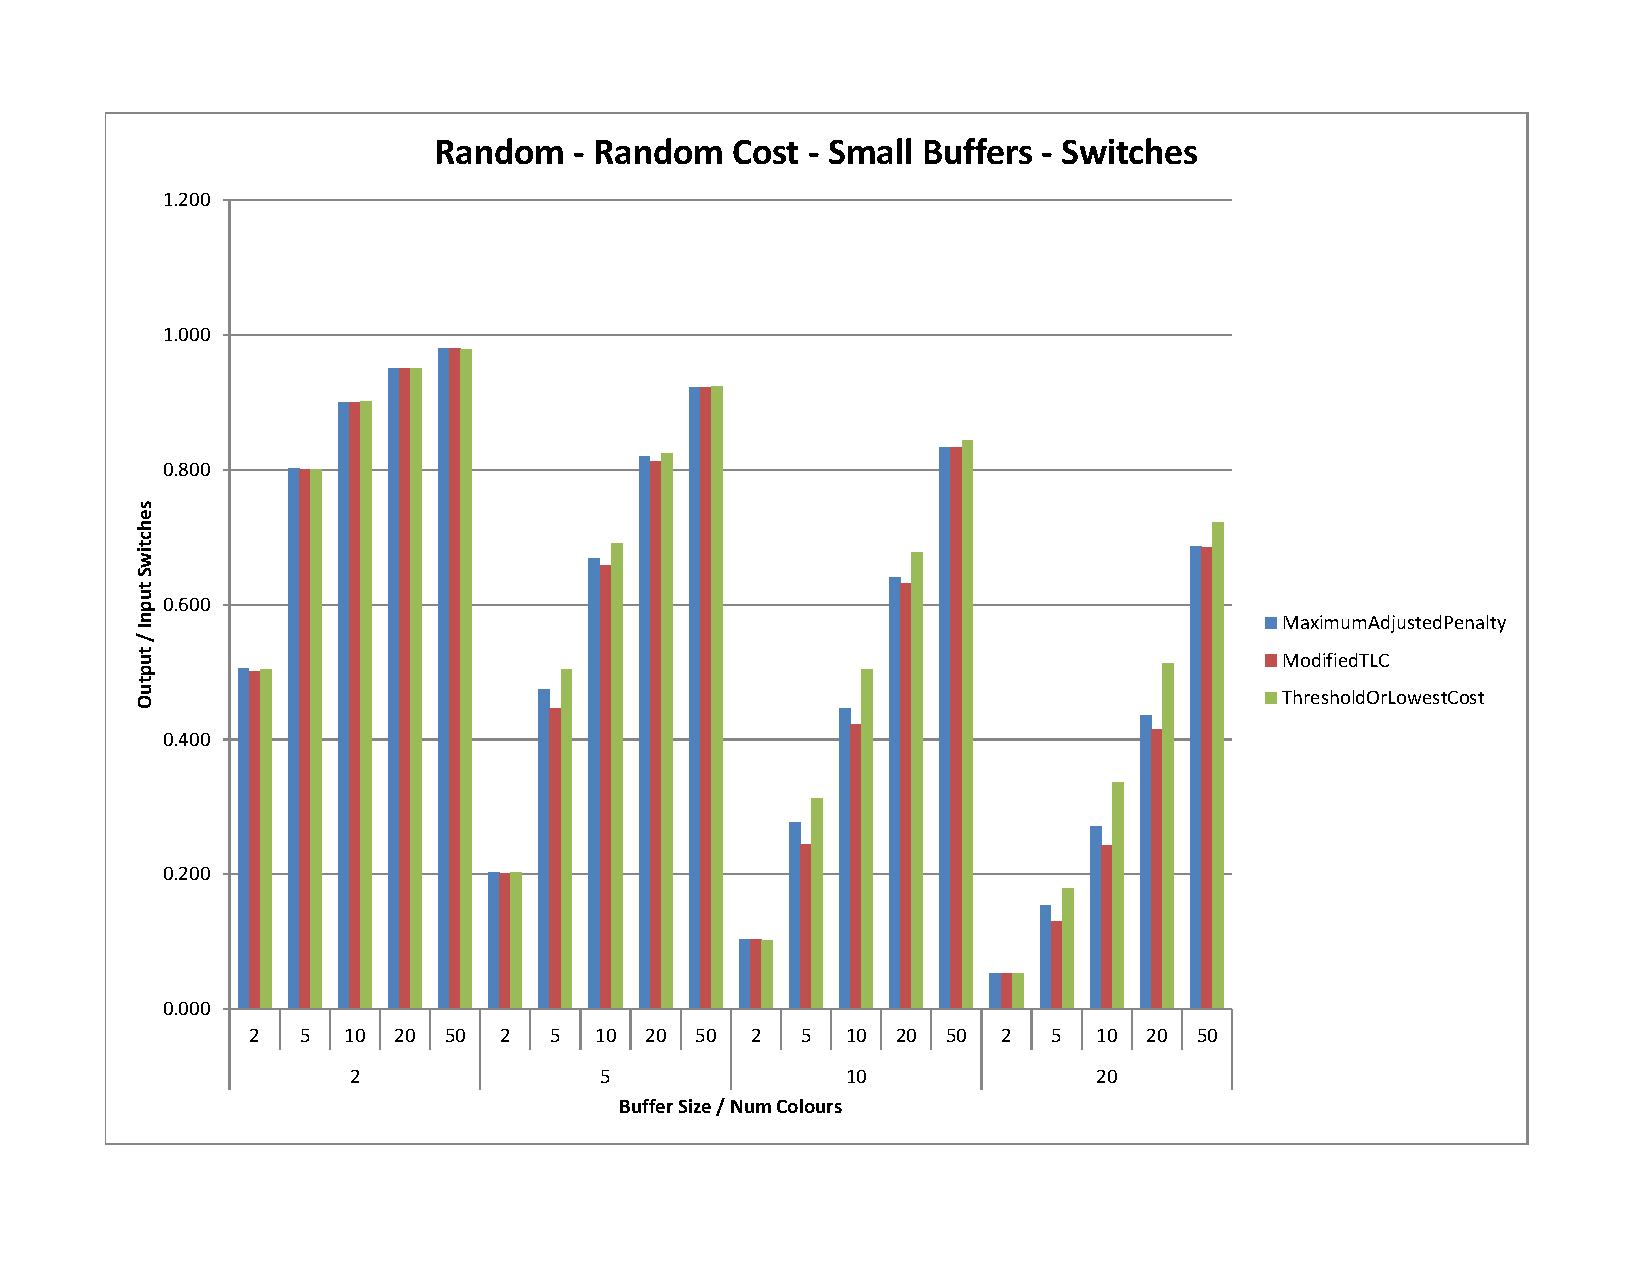
\includegraphics[scale=0.60]{Random-rc-small-switches.pdf}
\caption{TLC' achieves a better switch ratio than MAP and TLC}
\label{randomRCSmallSwitches}
\end{figure}   

While our results follow the similar trend of TLC' having a better switch ratio than TLC and MAP, and having a worse cost ratio than the others, for the case of Colour Difference cost function we observe that the cost ratios for TLC' are significantly higher than the cost ratios for MAP and TLC. This result is illustrated in Fig. TLC and MAP still continue to retain comparable cost ratios with only marginal differences. 

\begin{figure}[ht]
\centering 
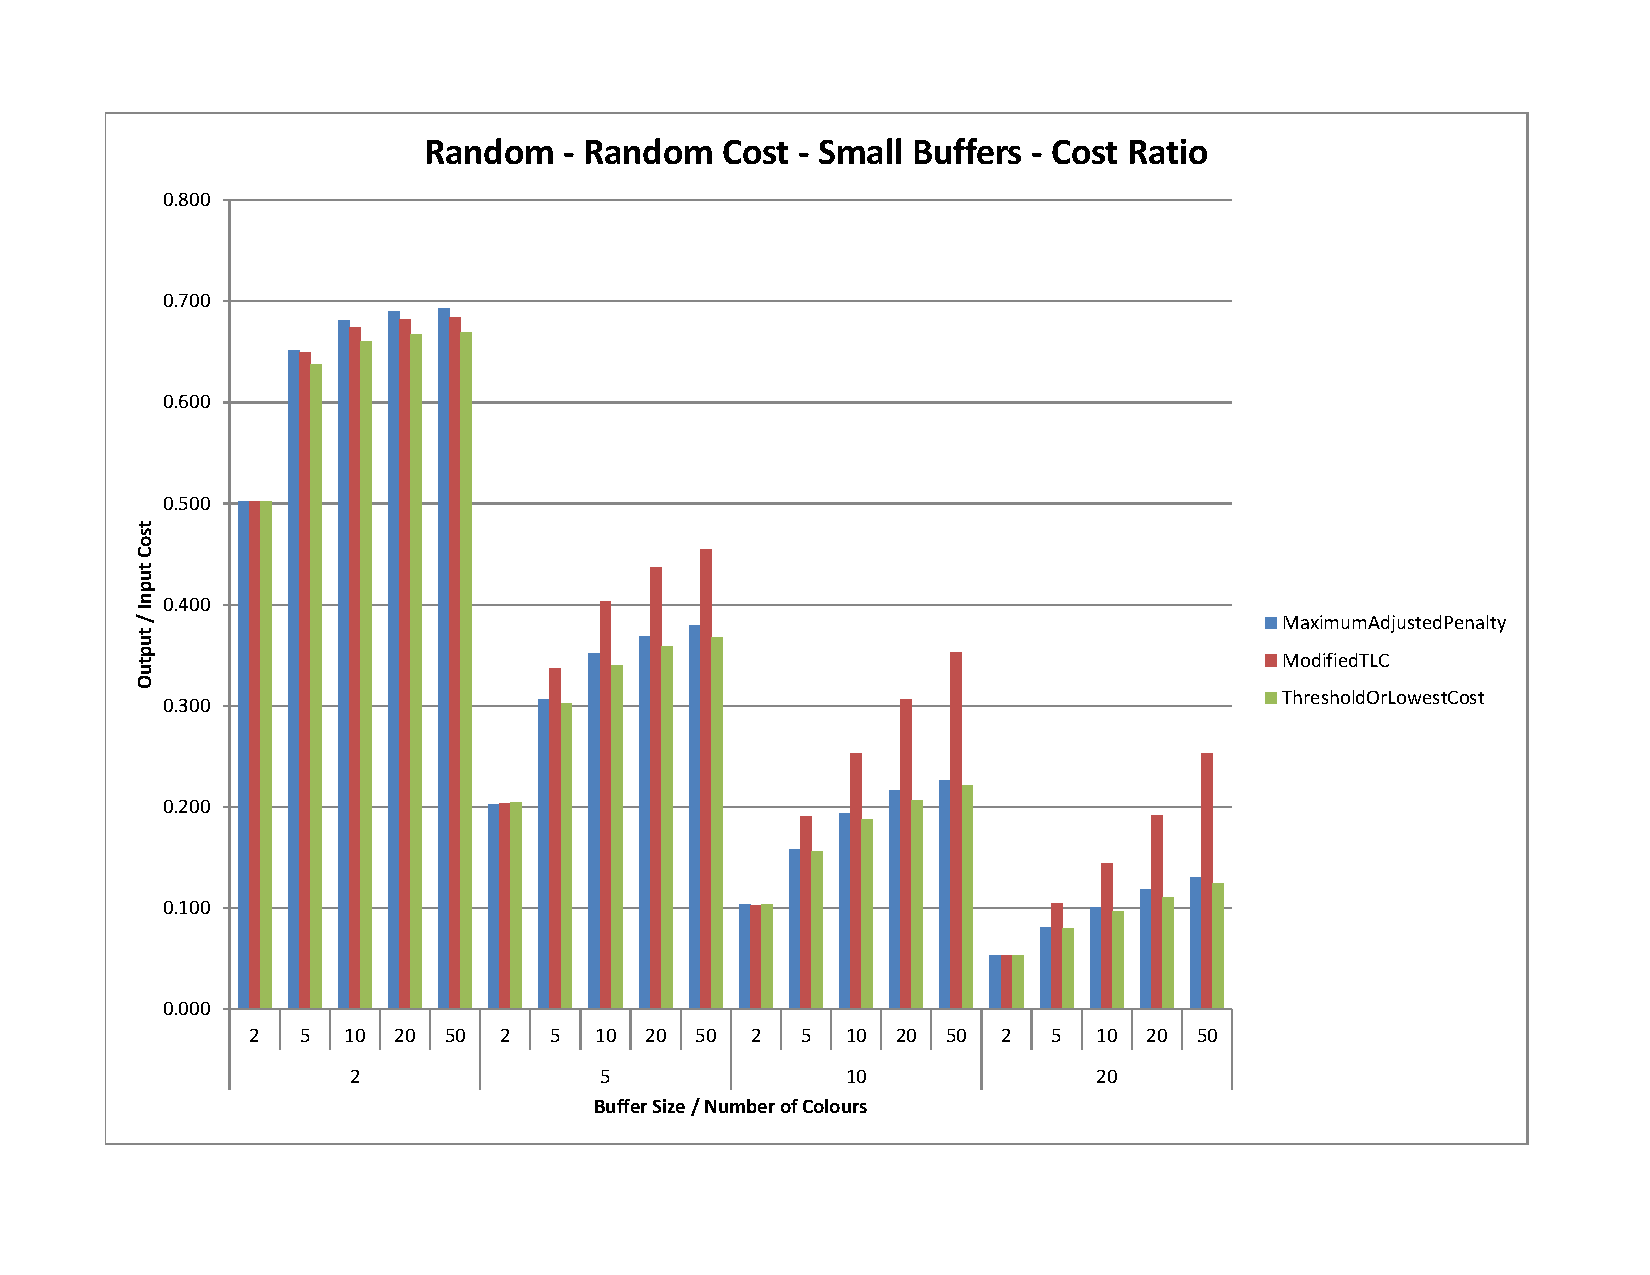
\includegraphics[scale=0.60]{Random-cd-small-cost.pdf}
\caption{TLC' has significantly higher cost ratios than TLC and MAP}
\label{randomCDSmallCost}
\end{figure}   

For the Uniform cost function, we observe that all our algorithms perform almost identically achieving almost the same reordering ratios for both switches and costs. We also observe that our algorithms do no achieve very significant reordering for large number of colours, as the reordering ratios are closer to 1.0. 

All our algorithms achieve a very good performance when comparing the reordering ratios for medium sized buffers. We observe that for the Cost Equals Colour and Cost Equals Quadratic Colour cost functions, TLC' has significantly lower switch ratios than TLC and MAP. When comparing cost ratios, we observe that TLC' does slightly better than TLC and MAP for both these cost functions. These results are illustrated in Fig. \ref{randomCCMedium Switches} and Fig. \ref{randomCQMediumCost}.

\begin{figure}[ht]
\centering 
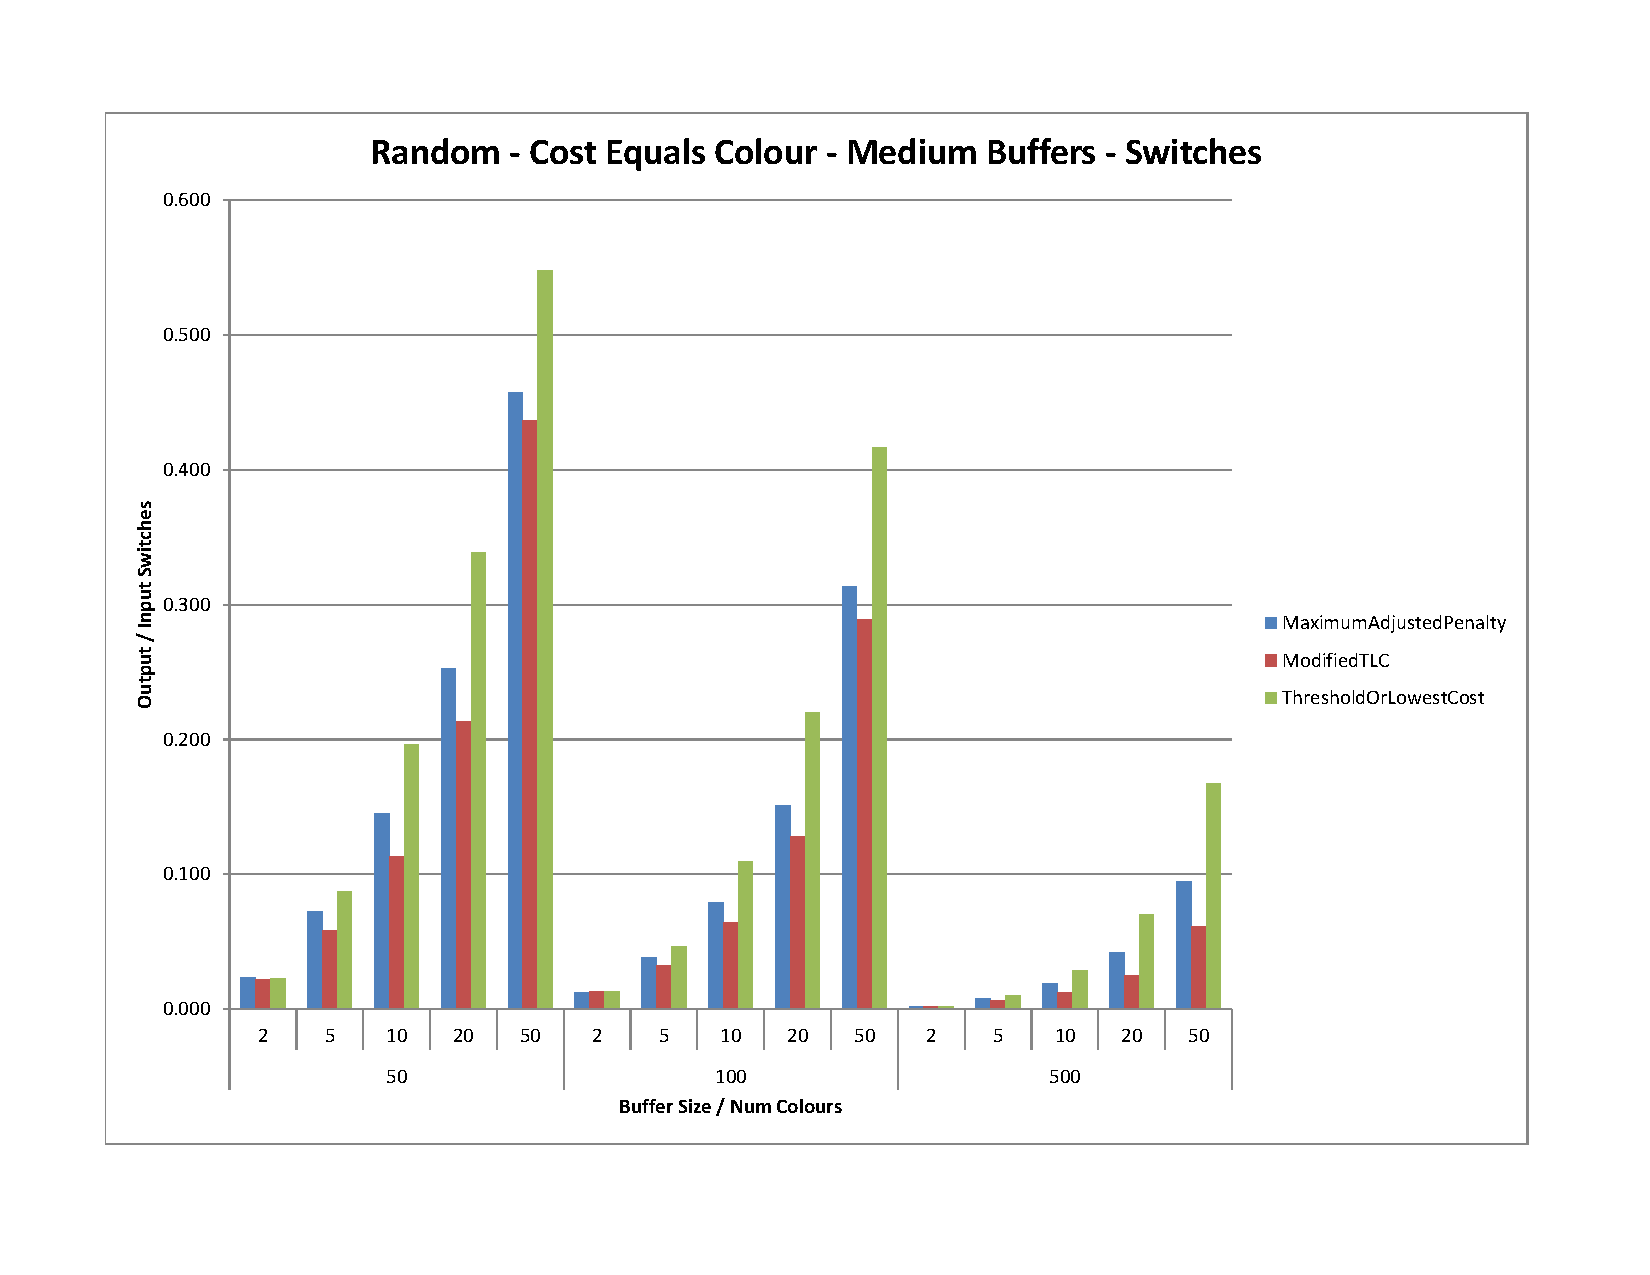
\includegraphics[scale=0.60]{Random-cc-medium-switches.pdf}
\caption{TLC' has significantly lower switch ratios than TLC and MAP}
\label{randomCCMedium Switches}
\end{figure}   

\begin{figure}[ht]
\centering 
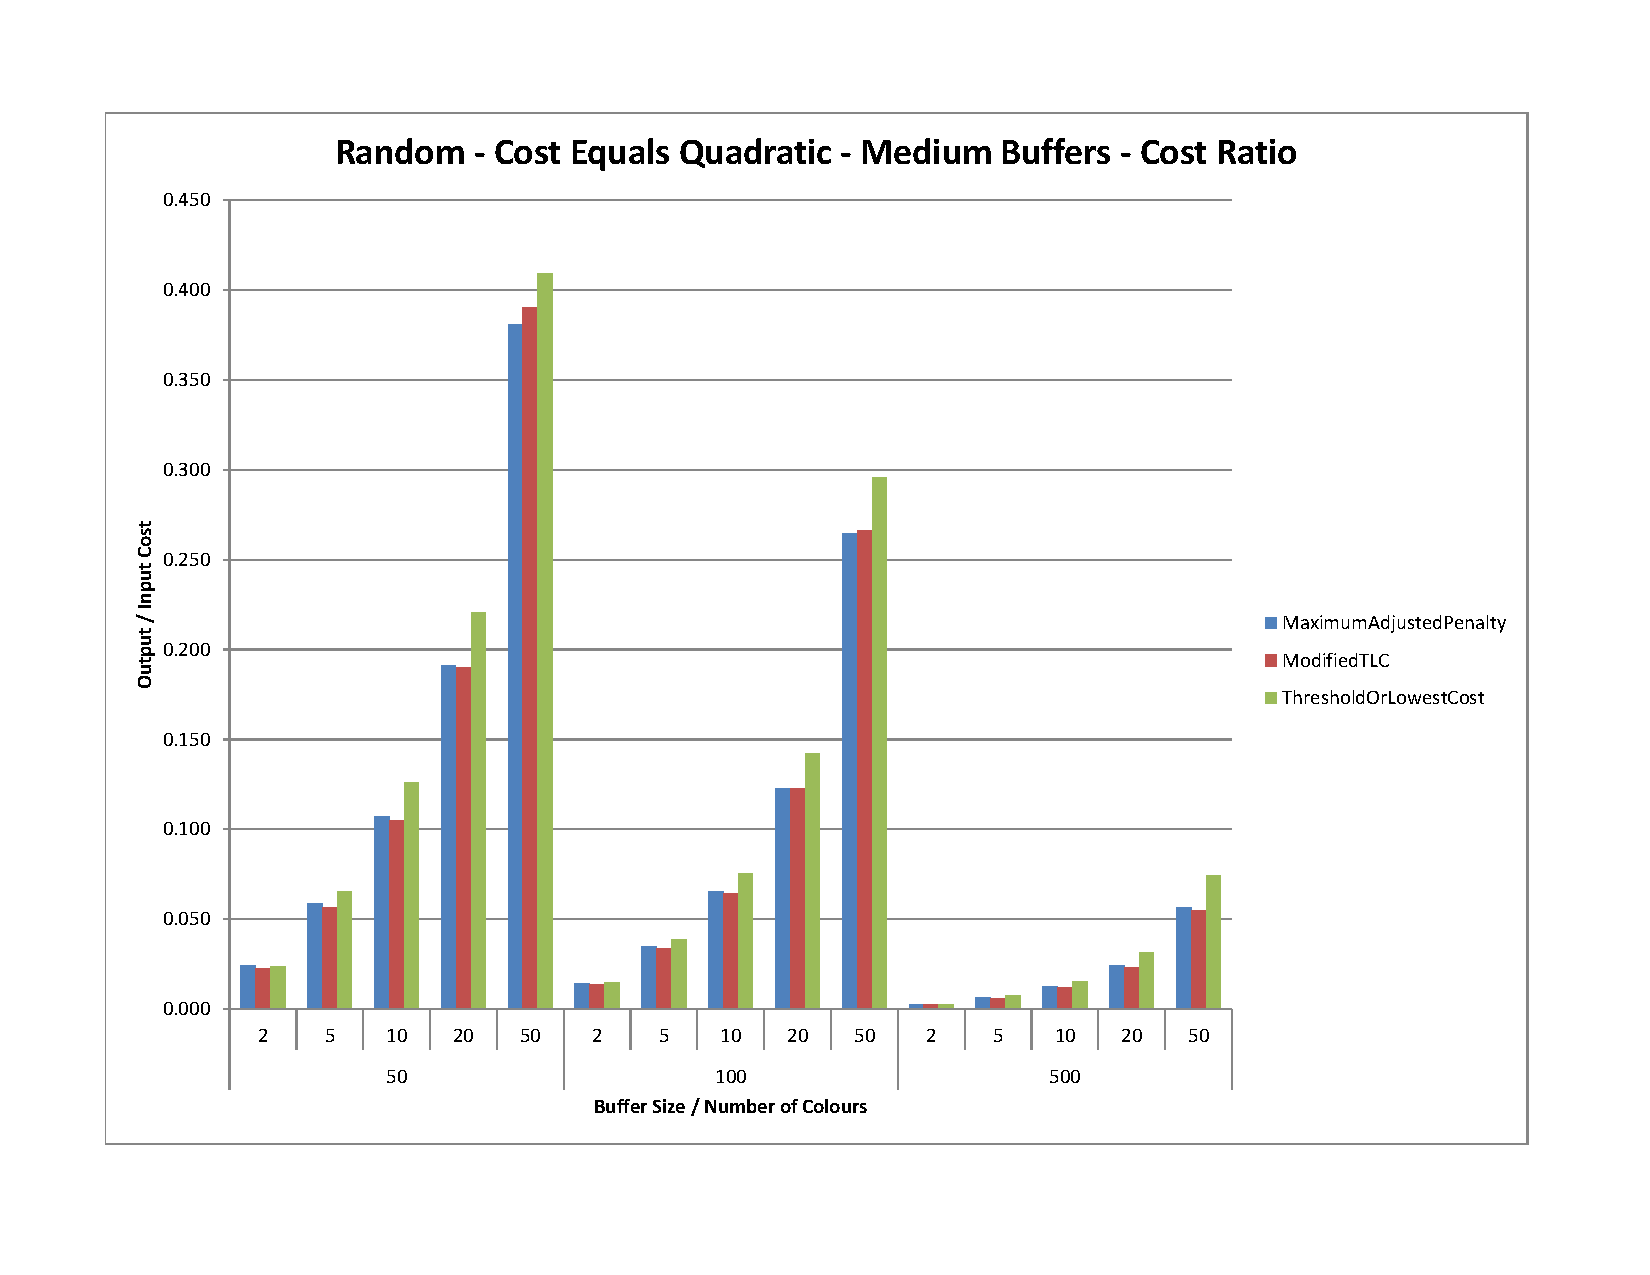
\includegraphics[scale=0.60]{Random-cq-medium-cost.pdf}
\caption{TLC' performs better than TLC and MAP when cost ratios are compared}
\label{randomCQMediumCost}
\end{figure}   

This trend where TLC' has a significantly lower switch ratio than MAP and TLC and where TLC' performs slightly better than TLC and MAP when cost ratios are compared extends to the Random cost function as well. Similar figures can be plotted to reveal this behaviour. 

While all our algorithms perform extremely well for the Colour Difference cost function, we observe that TLC' has a significantly higher cost ratio when compared to TLC and MAP. However, we also observe that TLC' has fewer switches for exactly the same buffer size/number of colours combinations. MAP performs slightly worse than TLC making TLC the best algorithm for the Colour Difference cost function. 

For the Uniform cost function, we observe that all our algorithms have very comparable reordering ratios, with MAP performing slightly better than TLC and TLC' in some cases. 

\subsubsection{Random Block Sequences}

All our algorithms achieve very comparable performance when comparing the cost ratio for the Cost Equals Colour cost function. Since the input sequence comes in variable sized blocks, all our algorithms can achieve a good reordering ratio only when the size of the blocks are small. This can happen only when the number of colours are small since the block size increases as the number of colours increases. This is reflected in the results obtained where we see that the cost and switch ratios are closer to 1.0 for large number of colours and our algorithms achieve a good performance otherwise. When comparing the switch ratios, we observe that TLC' achieves a better performance than MAP and TLC for small buffer sizes with few colours, MAP and TLC have comparable performance with MAP doing marginally better in most cases. This is illustrated in Fig. \ref{randomBlockCCSmallSwitches}.

\begin{figure}[ht]
\centering 
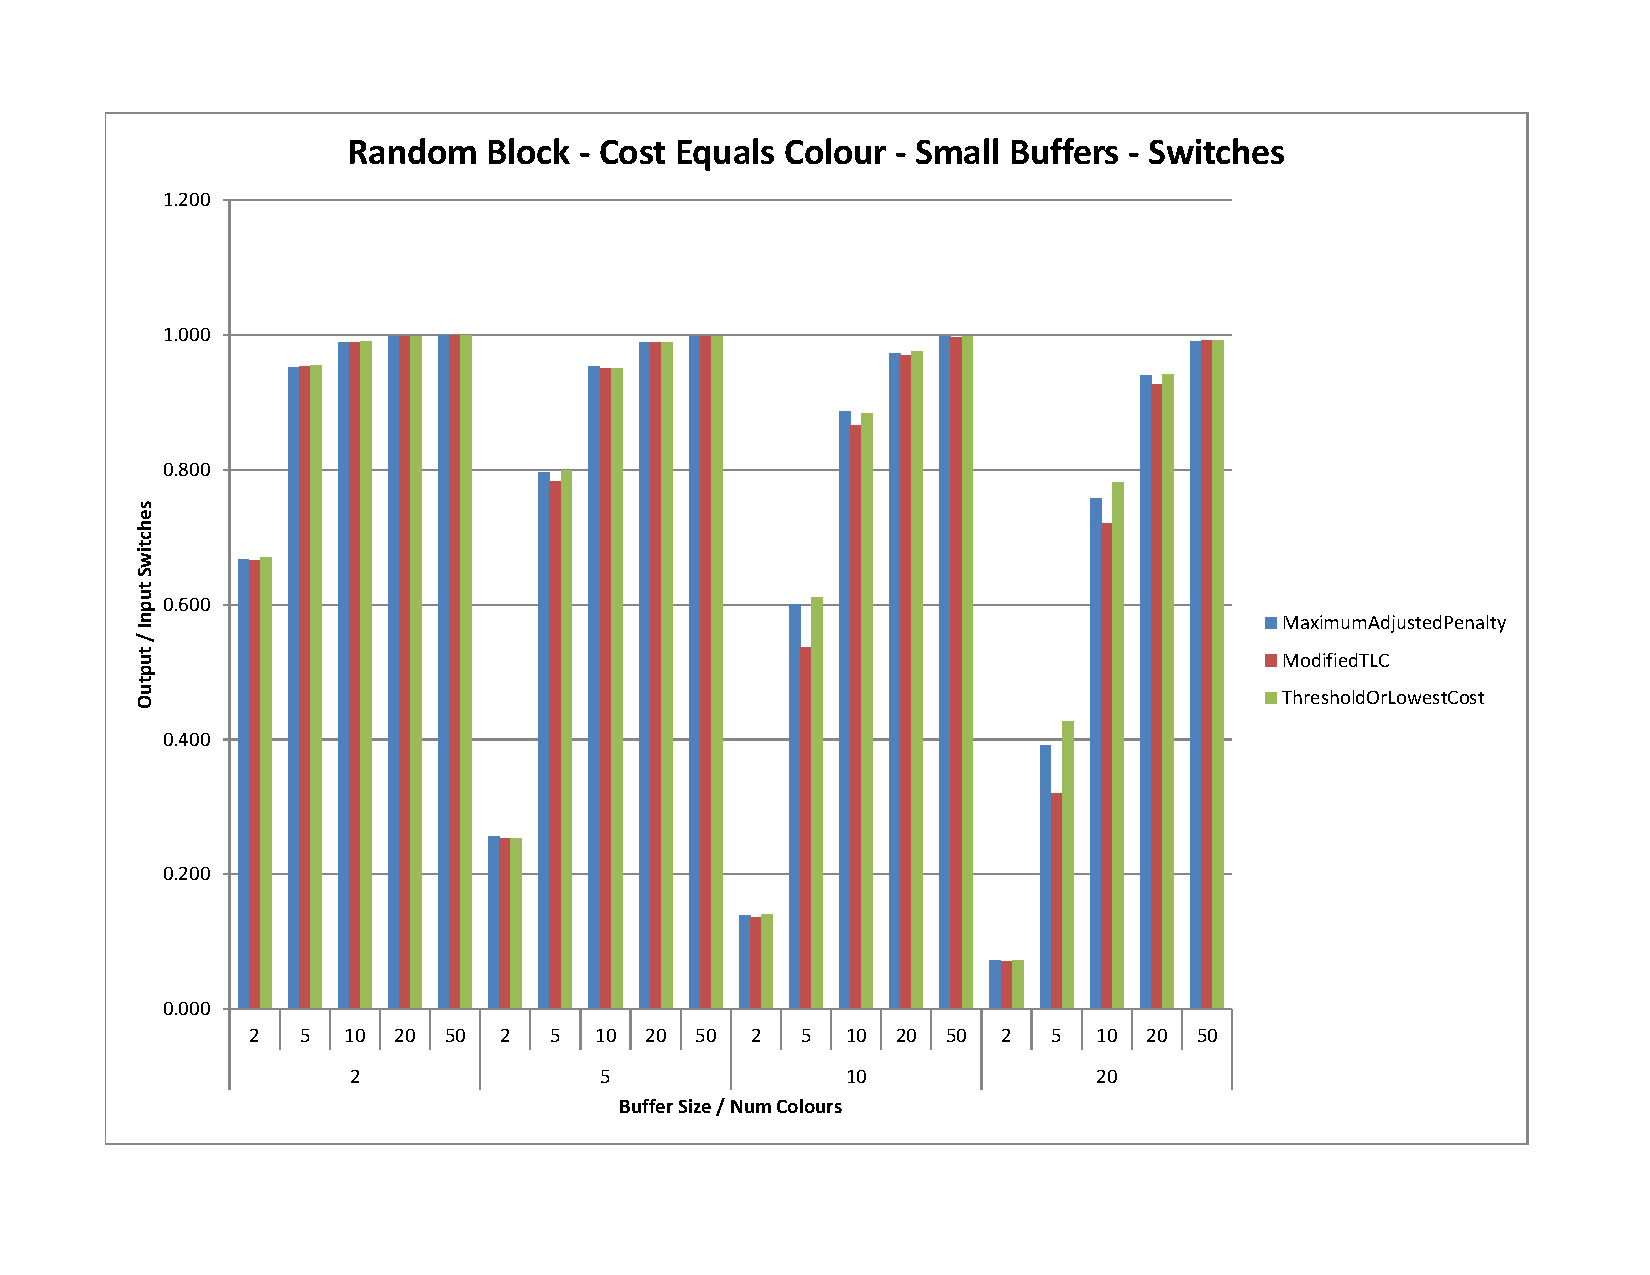
\includegraphics[scale=0.60]{Random-Block-cc-small-switches.pdf}
\caption{TLC' achieves a better switch ratio than MAP and TLC for small number of colours}
\label{randomBlockCCSmallSwitches}
\end{figure}   

We observe a similar trend as with the Cost Equals Quadratic Colour cost function where TLC' achieves a better switch ratio than TLC and MAP. When comparing cost ratios we observe that all our algorithms achieve very comparable ratios with TLC doing marginally better than  MAP and TLC' in most cases. 

Staying consistent with the trend, Random cost function also exhibits a similar behaviour where all our algorithms have extremely comparable performance, performing only marginally better or worse than the other when comparing cost ratios. This is illustrated in Fig. \ref{randomBlockRCSmallCost}. When comparing switch ratios, we observe that TLC' achieves a better switch ratio than MAP and TLC when the number of colours is less than the buffer size, MAP and TLC have very similar ratios with MAP performing marginally better. 

\begin{figure}[ht]
\centering 
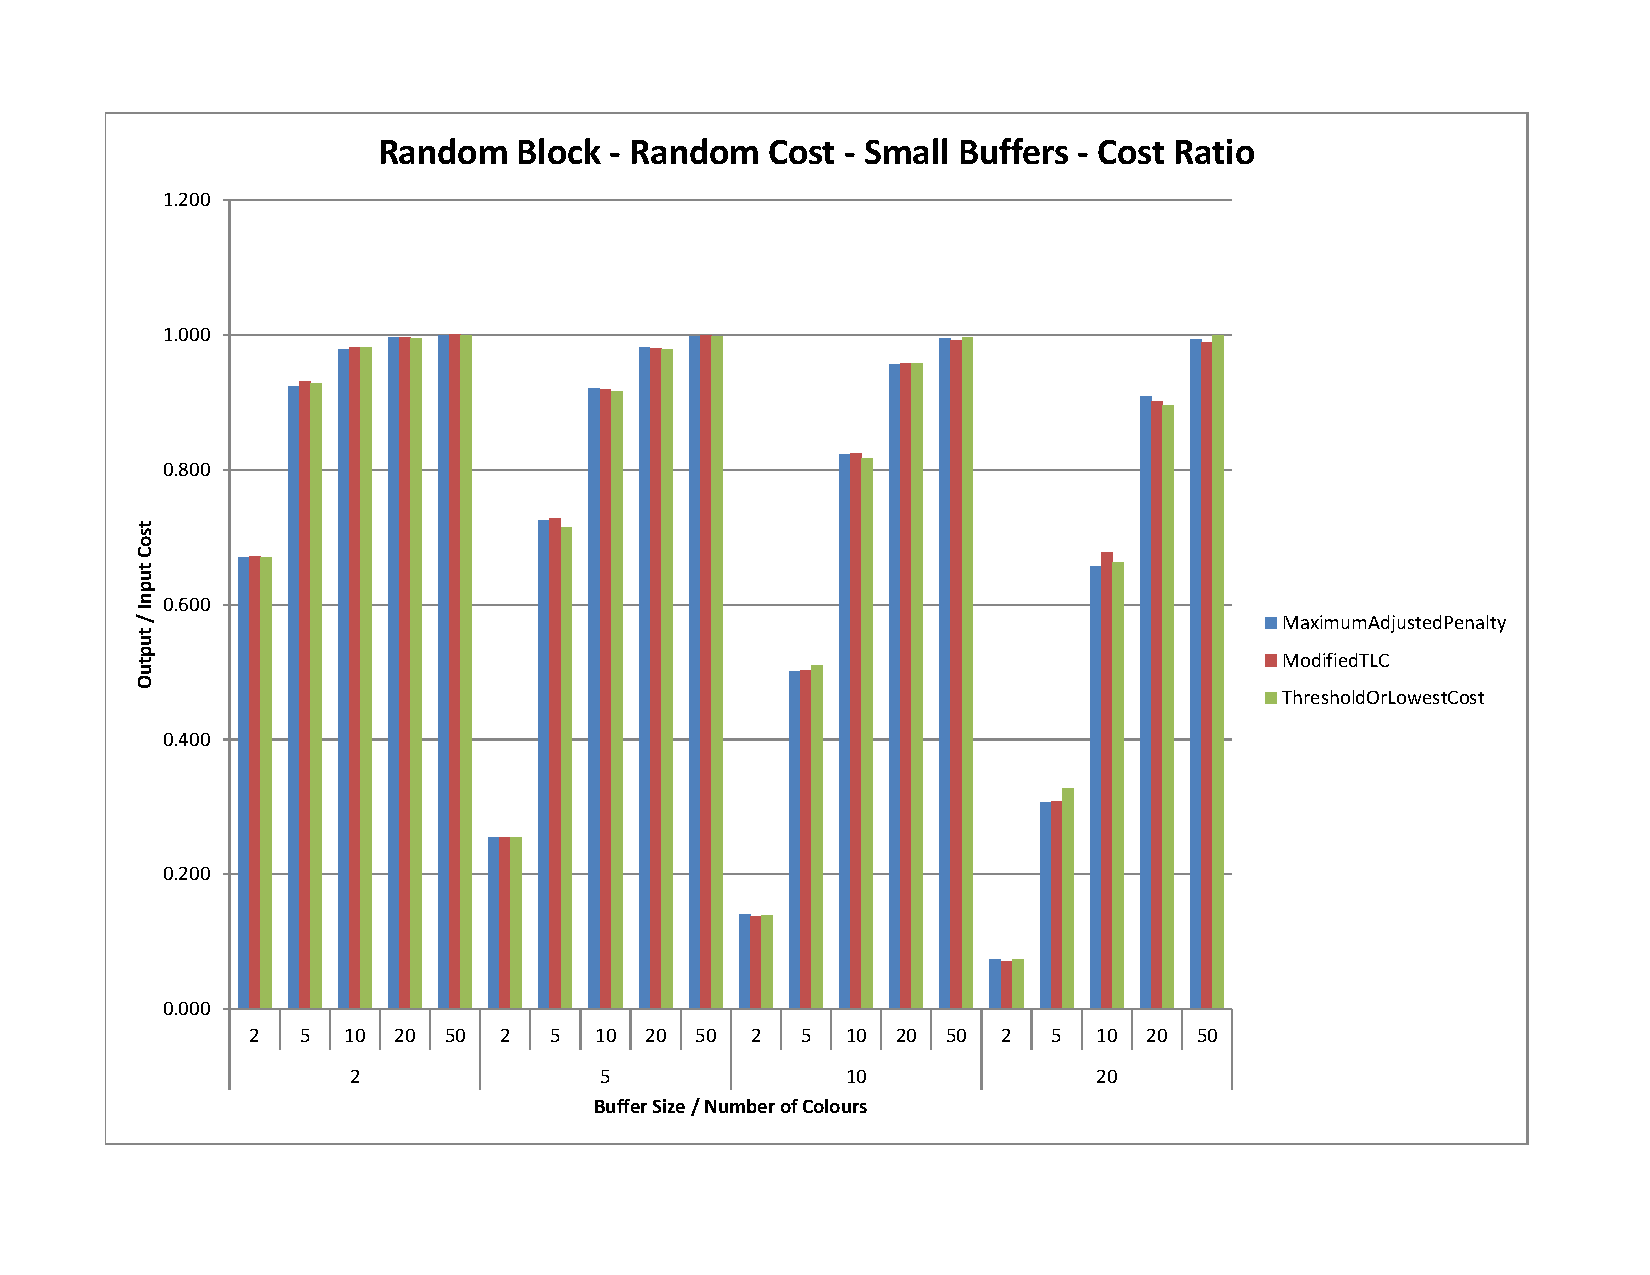
\includegraphics[scale=0.60]{Random-Block-rc-small-cost.pdf}
\caption{TLC' achieves a better switch ratio than MAP and TLC for small number of colours}
\label{randomBlockRCSmallCost}
\end{figure}   

All our algorithms have very comparable switch ratios for the Colour Difference cost function. As seen in the other cases, TLC' does slightly better when the number of colours is very small, but otherwise all our algorithms have very similar switch ratios. However, while comparing cost ratios we observe that TLC' performs poorly for this cost function, it has significantly higher cost ratios compared to TLC and MAP, which both have comparable cost ratios. 

In the case of Uniform cost function, we observe that all our algorithms have almost similar cost and switch ratios, with TLC' and MAP being almost identical in a few cases, TLC' performs marginally better than MAP and TLC in other cases and TLC has the marginally higher cost ratios for this cost function. However, overall, we observe that all our algorithms have comparable performance.  

As is the case with small buffers, we observe that the reordering ratios for all our algorithms are higher for large number of colours even in the case of medium buffers. This is expected behaviour since the block size increases as the number of colours increase leaving little scope for reordering. We observe that for the Cost Equals Colour cost function, TLC' achieves a better performance than TLC and MAP when both the cost and switch ratios are compared. 

We see a similar trend with the Cost Equals Quadratic Colour cost function, however, the similarity is only limited to the switch ratio comparison. As with the Cost Equals Colour cost function, we observe that TLC' has a better switch ratio than TLC and MAP, but when comparing the cost ratios we observe that there is no one algorithm that performs better than the other across all combinations. This is illustrated in Fig. \ref{randomBlockCQMediumCost}. Also, for buffer sizes 50 and 100, when the number of colours are 50, we observe that the cost ratio for MAP and TLC exceeds 1.0 indicating that reordering increases the cost. These details are explained in a later section. 

\begin{figure}[ht]
\centering 
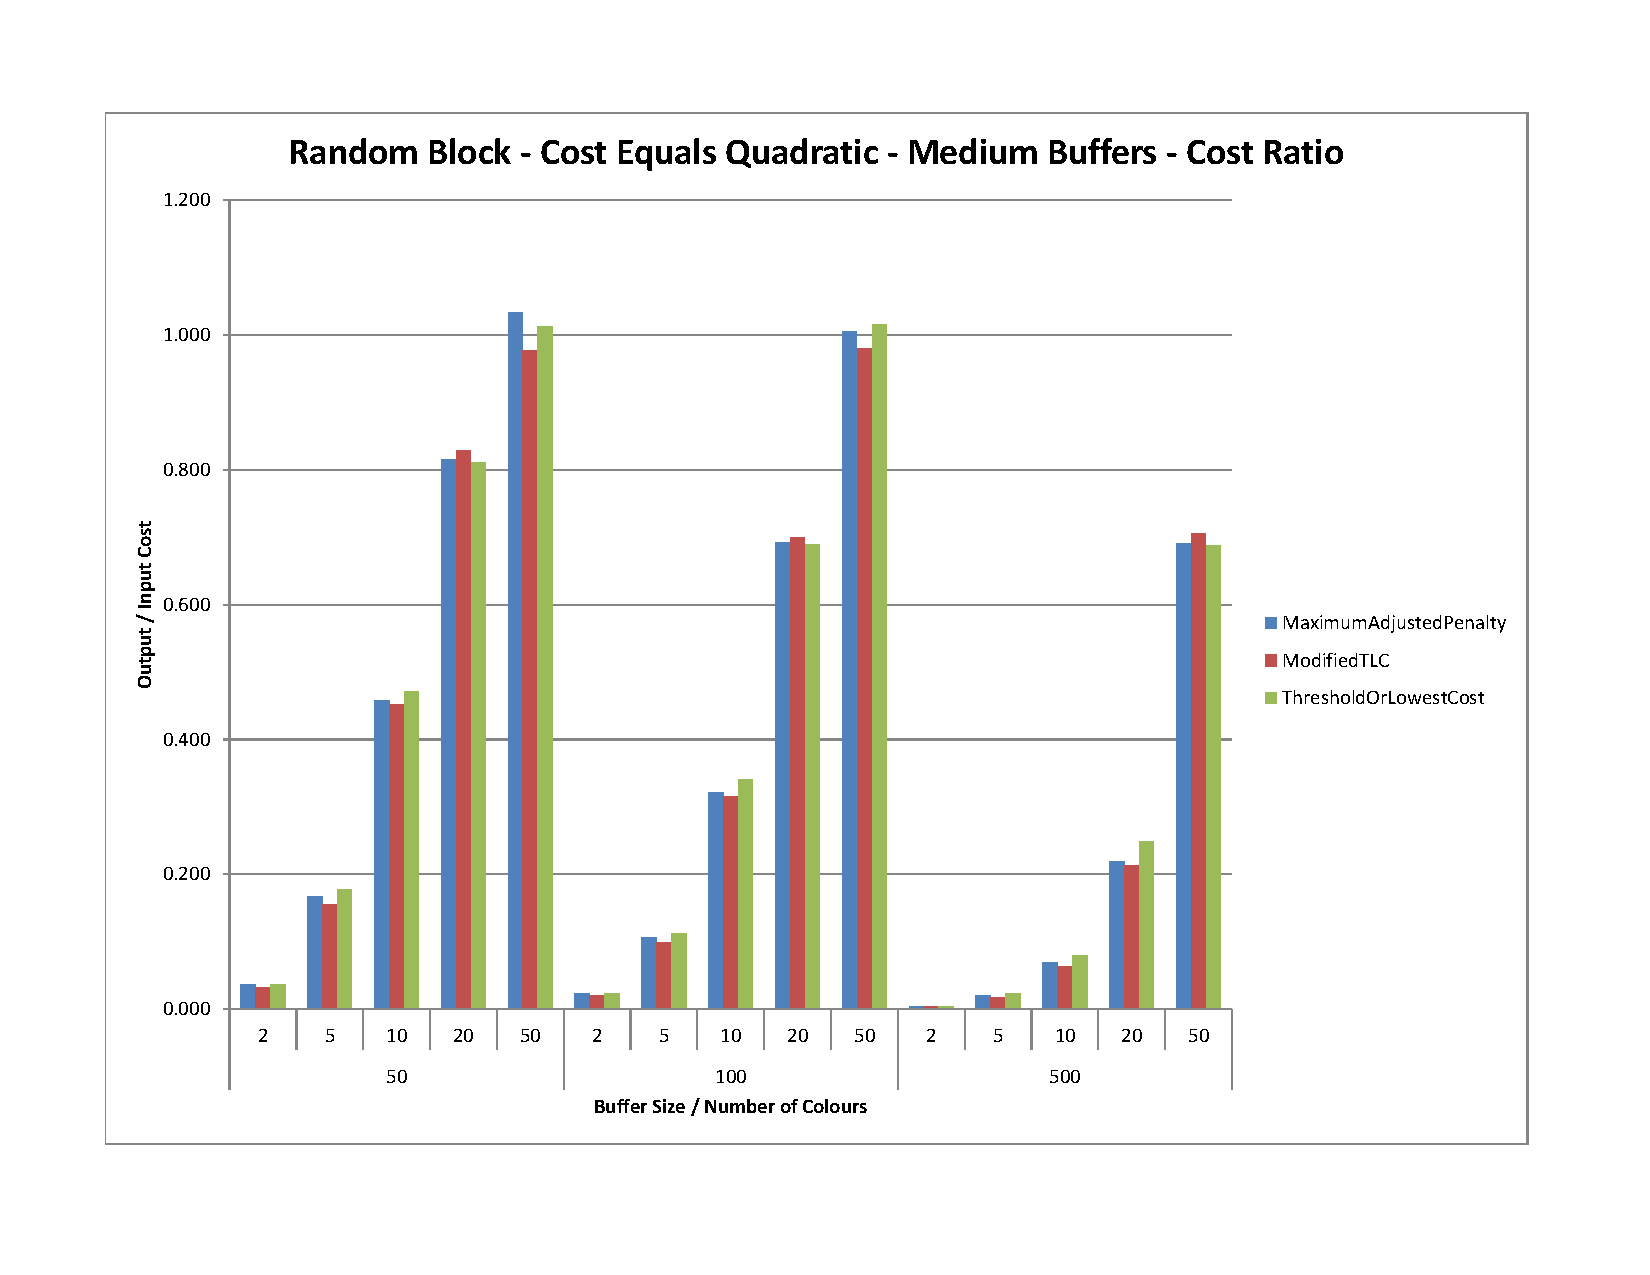
\includegraphics[scale=0.60]{Random-Block-cq-medium-cost.pdf}
\caption{All algorithms are comparable}
\label{randomBlockCQMediumCost}
\end{figure}   

For the Random cost function, we find that TLC' has a better performance than TLC and MAP when the number of colours is small compared to the buffer size ($ C < k$), when the switch ratios are compared. For all other cases all our algorithms have similar performance. When cost ratios are compared, we observe that TLC' has higher cost ratios than TLC and MAP when the number of colours increases. 

When comparing the switch ratio for the Colour Difference cost function, we observe that all our algorithms achieve very similar ratios indicating that they all have similar reordering performance.  However, when comparing the cost ratios, we observe that TLC' has significantly higher cost ratios than TLC and MAP, with the cost being more than two times the cost incurred for TLC and MAP. This result is illustrated in Fig. \ref{randomBlockCDMediumCost}.

\begin{figure}[ht]
\centering 
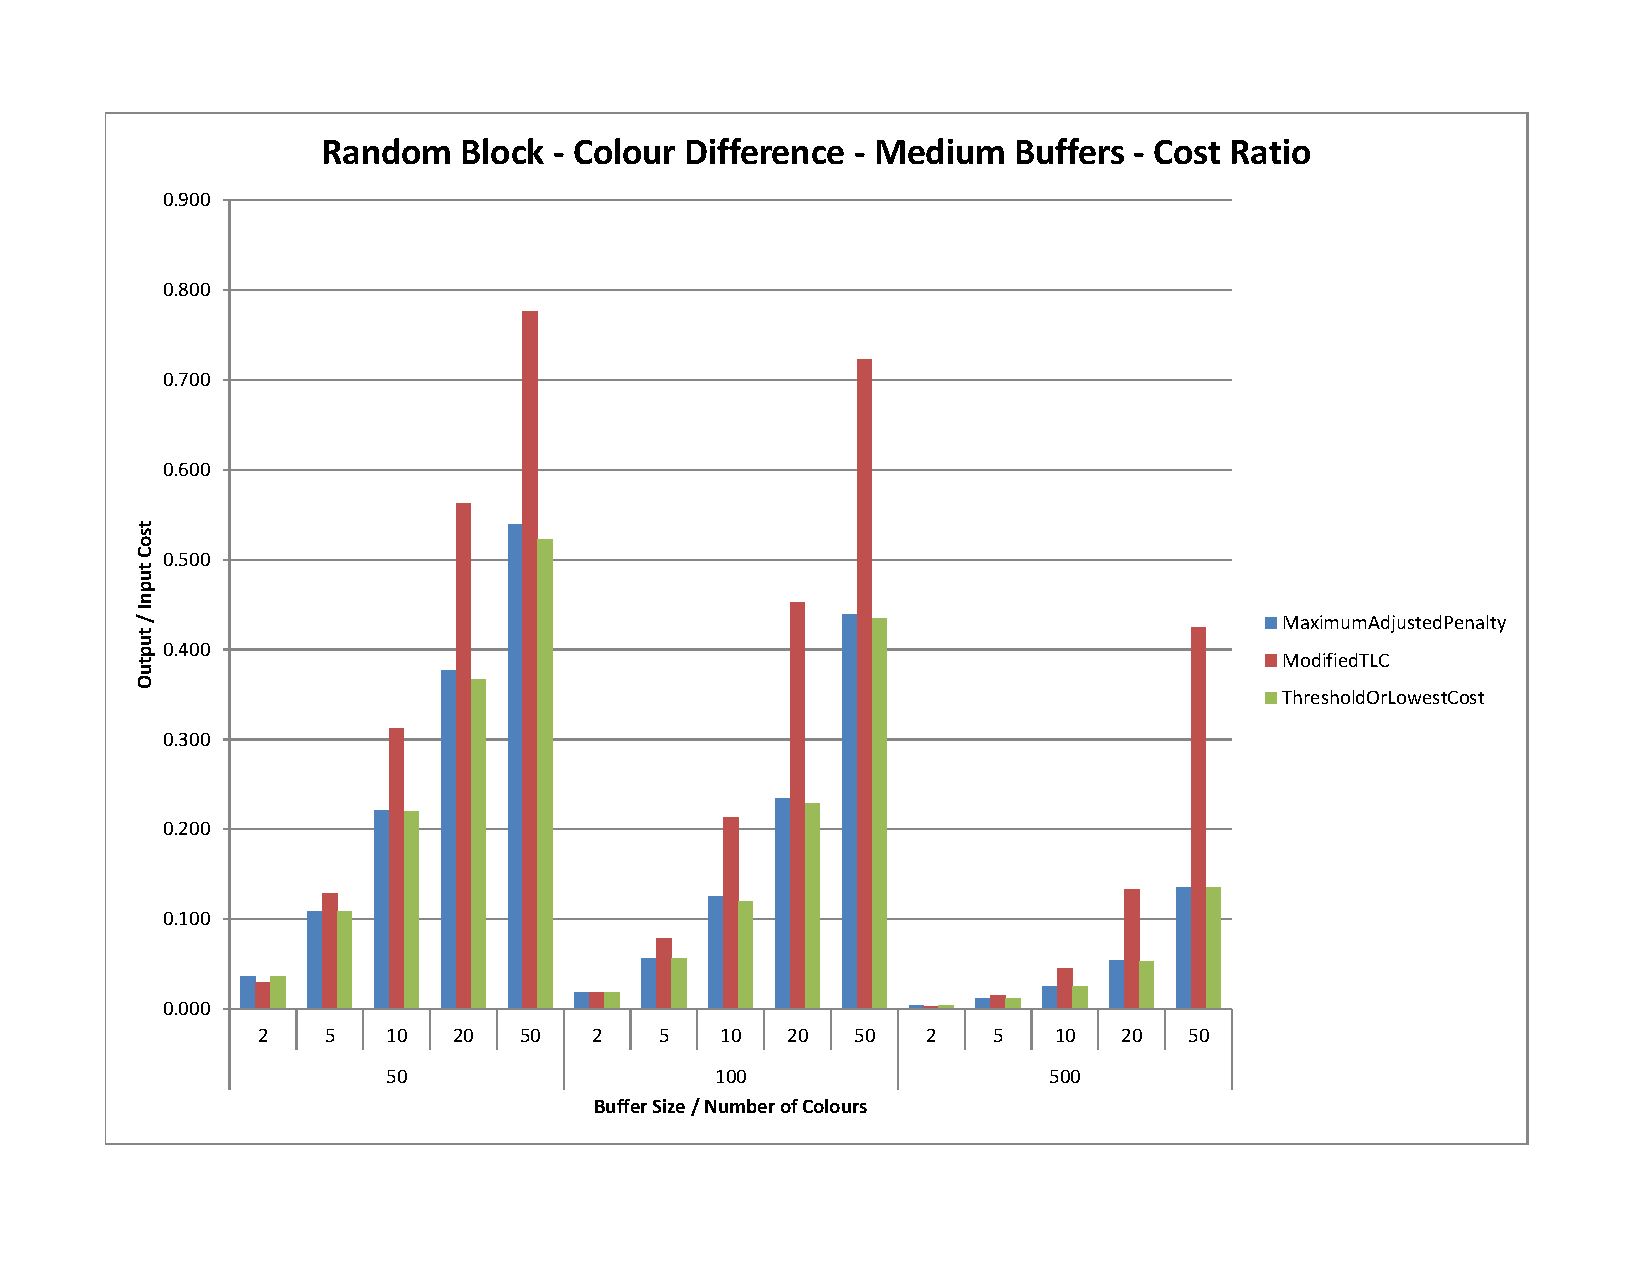
\includegraphics[scale=0.60]{Random-Block-cd-medium-cost.pdf}
\caption{The cost ratio for TLC' is more than two times the cost ratio for TLC and MAP}
\label{randomBlockCDMediumCost}
\end{figure}   

For Uniform cost function, all our algorithms have almost identical performance. 

\subsubsection{Sequential Block Sequences}

For the Cost Equals Colour cost function, out algorithms fail to permute the sequence for very small buffer sizes (2 and 5). All our algorithms have a switch and cost ratio of 1.0 indicating that the output sequence is identical to the input sequence. This behaviour is expected since our block sizes are 5 making it impossible for the algorithms to achieve any reordering. For buffer sizes 10 and 20, we observe that TLC achieves a better switch and cost ratio than MAP and TLC' when the number of colours is half the buffer size (that is for number of colours 5 and 10), while TLC' achieves a better performance than MAP and TLC for buffer size 20 and 5 colours. In all other cases we do not see any reordering as the number of colours and block sized nature of the input sequence does not permit any reordering. 

As seen in the case of Cost Equals Colour cost model, the Cost Equals Colour Quadratic Coloir cost function also witnesses no reordering for very small buffer sizes (2 and 5). However, for buffer sizes 10 and 20, our algorithms achieve reordering ratios close to 1.0 indicating that there has been no significant reordering. For buffer size 20, TLC achieves the best switch and cost ratios as long as the number of colours are less than or equal to the buffer size. It is interesting to note that while TLC and MAP achieve some reordering for buffer sizes 10 and 20 when the number of colours is 5 and 10, TLC' fails to reorder the input sequence thereby having switch and cost ratios as 1.0. This is illustrated in Fig. \ref{sequentialBlockCQSmallCost}.

\begin{figure}[ht]
\centering 
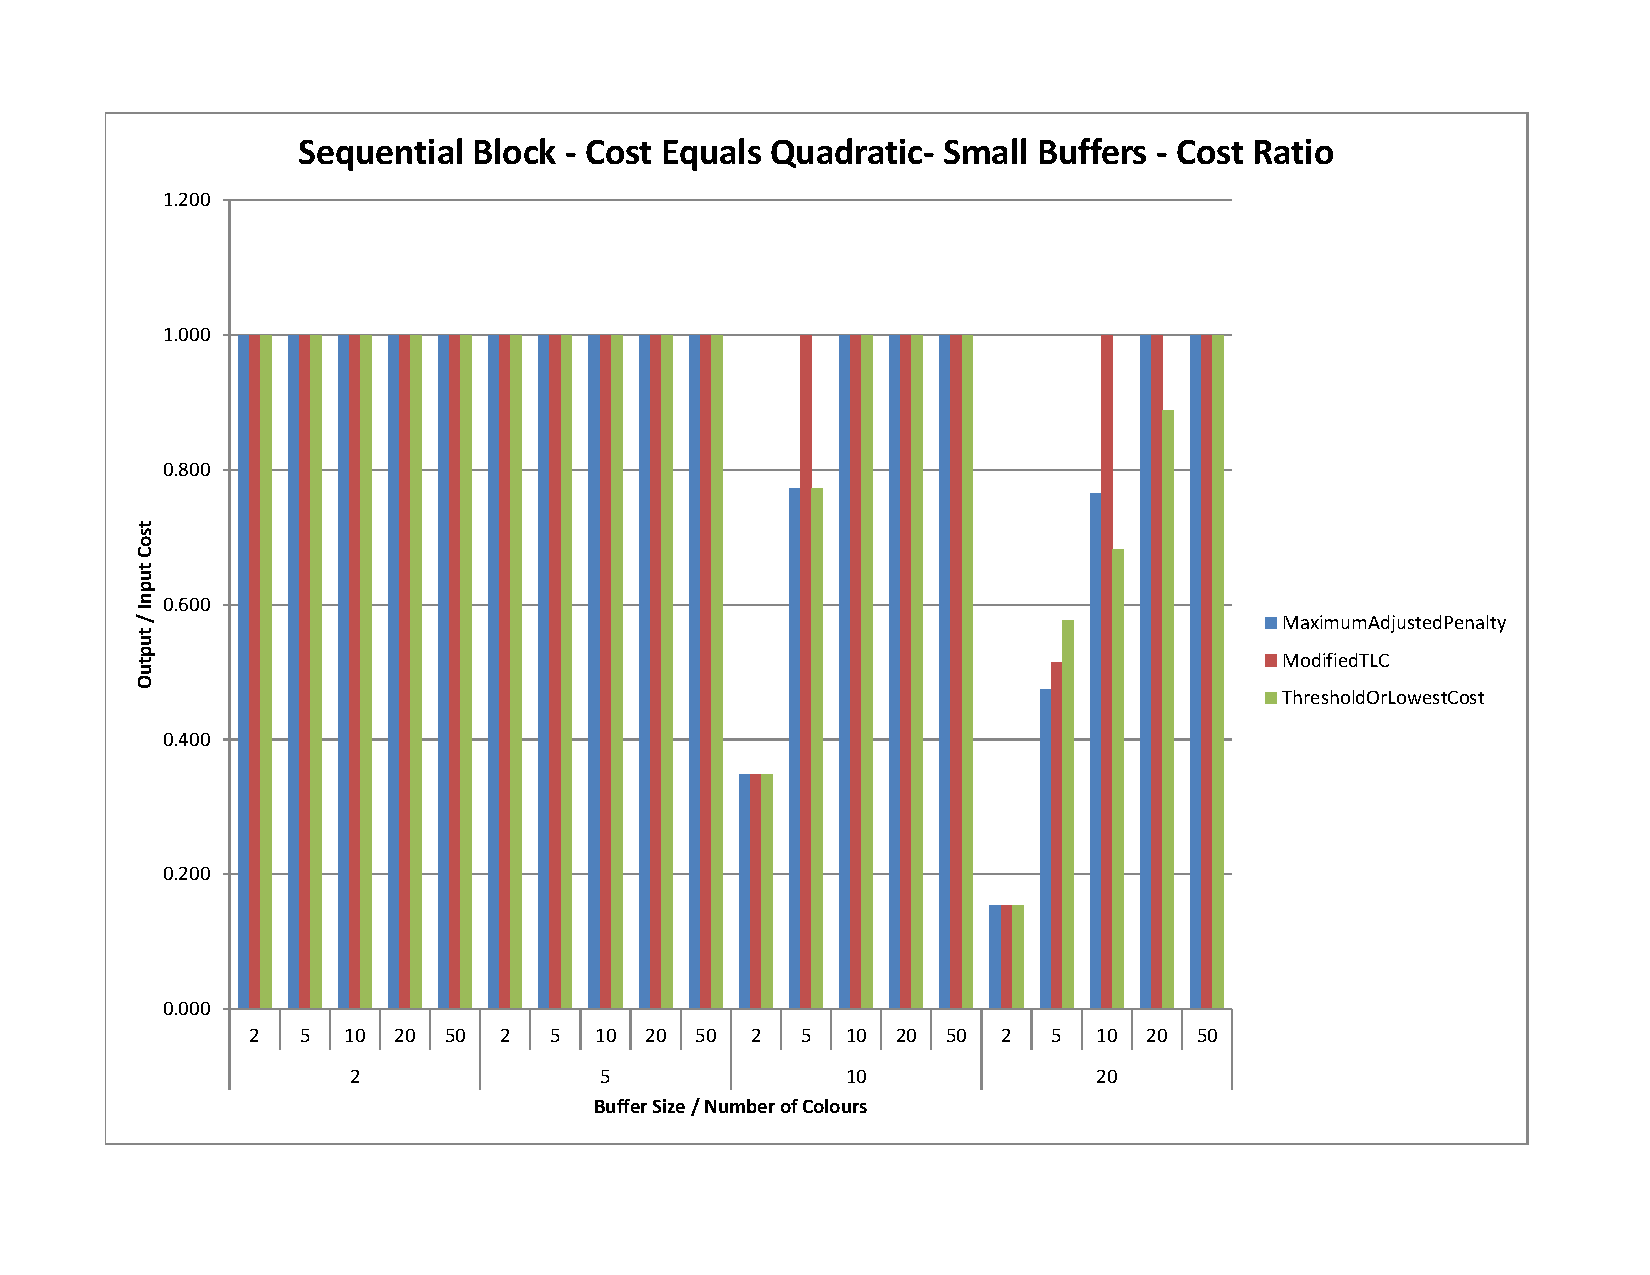
\includegraphics[scale=0.60]{Sequential-Block-cq-small-cost.pdf}
\caption{TLC' fails to permute for $k = 10, 20 and C = 5, 10$}
\label{sequentialBlockCQSmallCost}
\end{figure}   

Random cost function follows a similar trend where TLC' fails to achieve any reordering for exactly the same combination of buffer sizes and number of colours ($k = 10, 20$ and $C = 5, 10$). TLC and MAP achieve some reordering in this case with TLC performing better than MAP. However, for the Random cost function we also observe that the cost ratio for all our algorithms exceed 1.0 very marginally (of the order of 1.005) indicating that the cost of the output sequence is higher than the cost of the input sequence, this is analyzed in a later section. 

For the Colour Difference cost function, we observe that all our algorithms achieve exactly the same cost ratios for all combinations of small buffer sizes and number of colours. This trend continues when we compare the switch ratios as well except for the case when the buffer size is 20 and the number of colours is 5, in this scenario, we observe that TLC' achieves a better switch ratio than TLC and MAP, followed by MAP and then TLC. This is the only case where we observe different reordering ratios, all our algorithms have identical performance otherwise. This is illustrated in Fig. \ref{sequentialBlockCDSmallSwitches}. 

\begin{figure}[ht]
\centering 
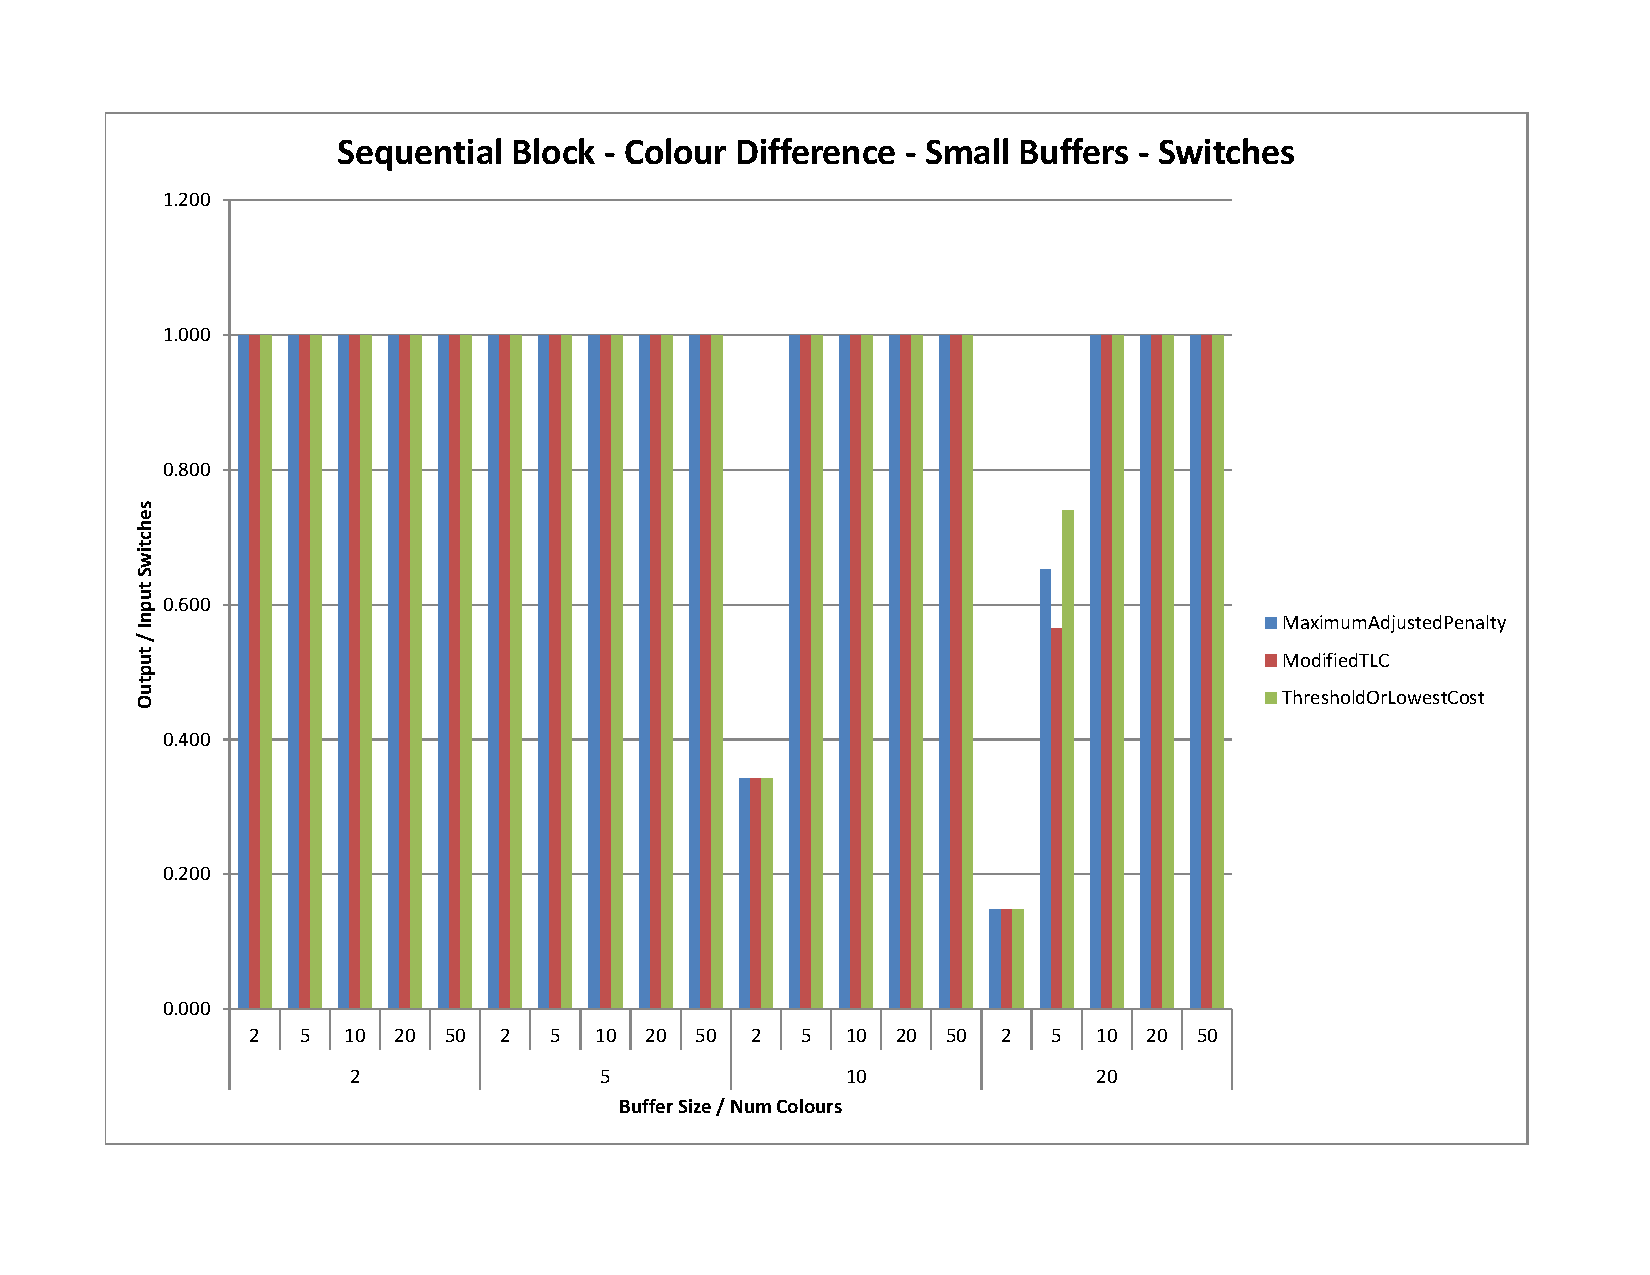
\includegraphics[scale=0.60]{Sequential-Block-cd-small-switches.pdf}
\caption{Non-identical switch ratio for $k = 20$ and $C = 5$}
\label{sequentialBlockCDSmallSwitches}
\end{figure}   

All our algorithms achieve exactly the same reordering ratios for the Uniform cost function, except for the case when the buffer size ($k = 20$ and $C = 5$), where MAP performs significantly better than TLC and TLC'. In this case TLC and TLC' fail to achieve any reordering of the input sequence. It may be noted that this is exactly the same buffer size/number of colours combination that had a non-identical performance in the Colour Difference cost model. 

For medium buffers, when comparing the switch ratios for the Cost Equals Colour cost function, TlC' has a better switch ratio than MAP and TLC when the number of colours is about half the size of the buffer. However, when comparing cost ratios we observe that TLC' has a better performance than MAP and TLC only when the number of colours is one-tenth of the size of the buffer. For all other cases,  TLC and MAP have a better performance than TLC'.

The exact same trend continues for the Cost Equals Quadratic Colour cost function where TLC' has a better switch ratio than MAP and TLC when the buffer size is 5 times the number of colours; for cost ratios, the buffer size is 10 times the number of colours. This result is illustrated in Fig. for switch ratio comparison. 

\begin{figure}[ht]
\centering 
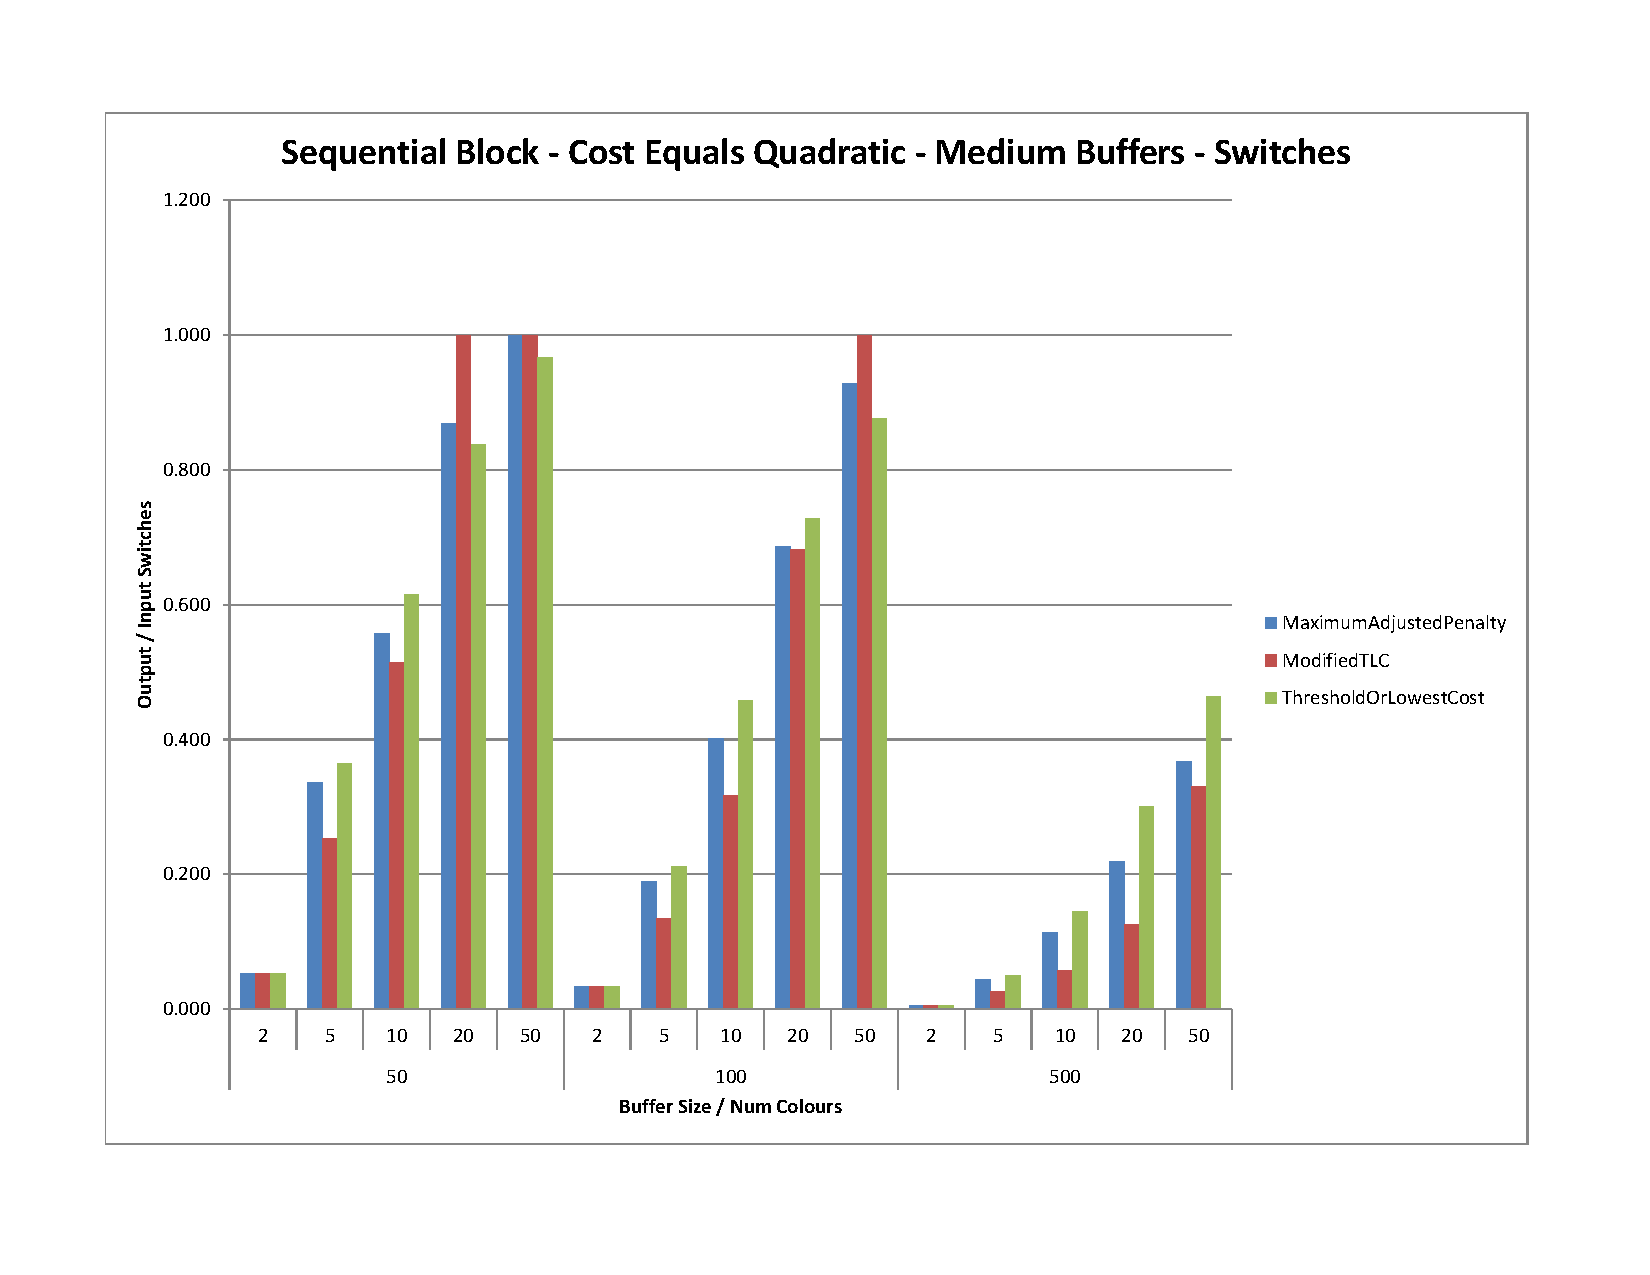
\includegraphics[scale=0.60]{Sequential-Block-cq-medium-switches.pdf}
\caption{TLC' has better switch ratio when $k >= 5 \times C$}
\label{sequentialBlockCQMediumSwitches}
\end{figure}   

For the Random cost function, we observe the exact same trend as we have seen in the Cost Equals Colour and Cost Equals Quadratic Colour cost functions, except that when comparing cost ratios, we observe that for buffer sizes 50 and 100 and when the number of colours are 20 and 50, the cost ratios for MAP and TLC are marginally more than 1.0 indicating that the reordering has increased the cost. These details are analyzed in a later section. 

For the Colour Difference cost funtion, we observe that TLC' has a better switch ratio than MAP and TLC, but the cost ratio is significantly higher for the cases where the switch ratio is lower. This is illustrated in Fig. 

\begin{figure}[ht]
\centering 
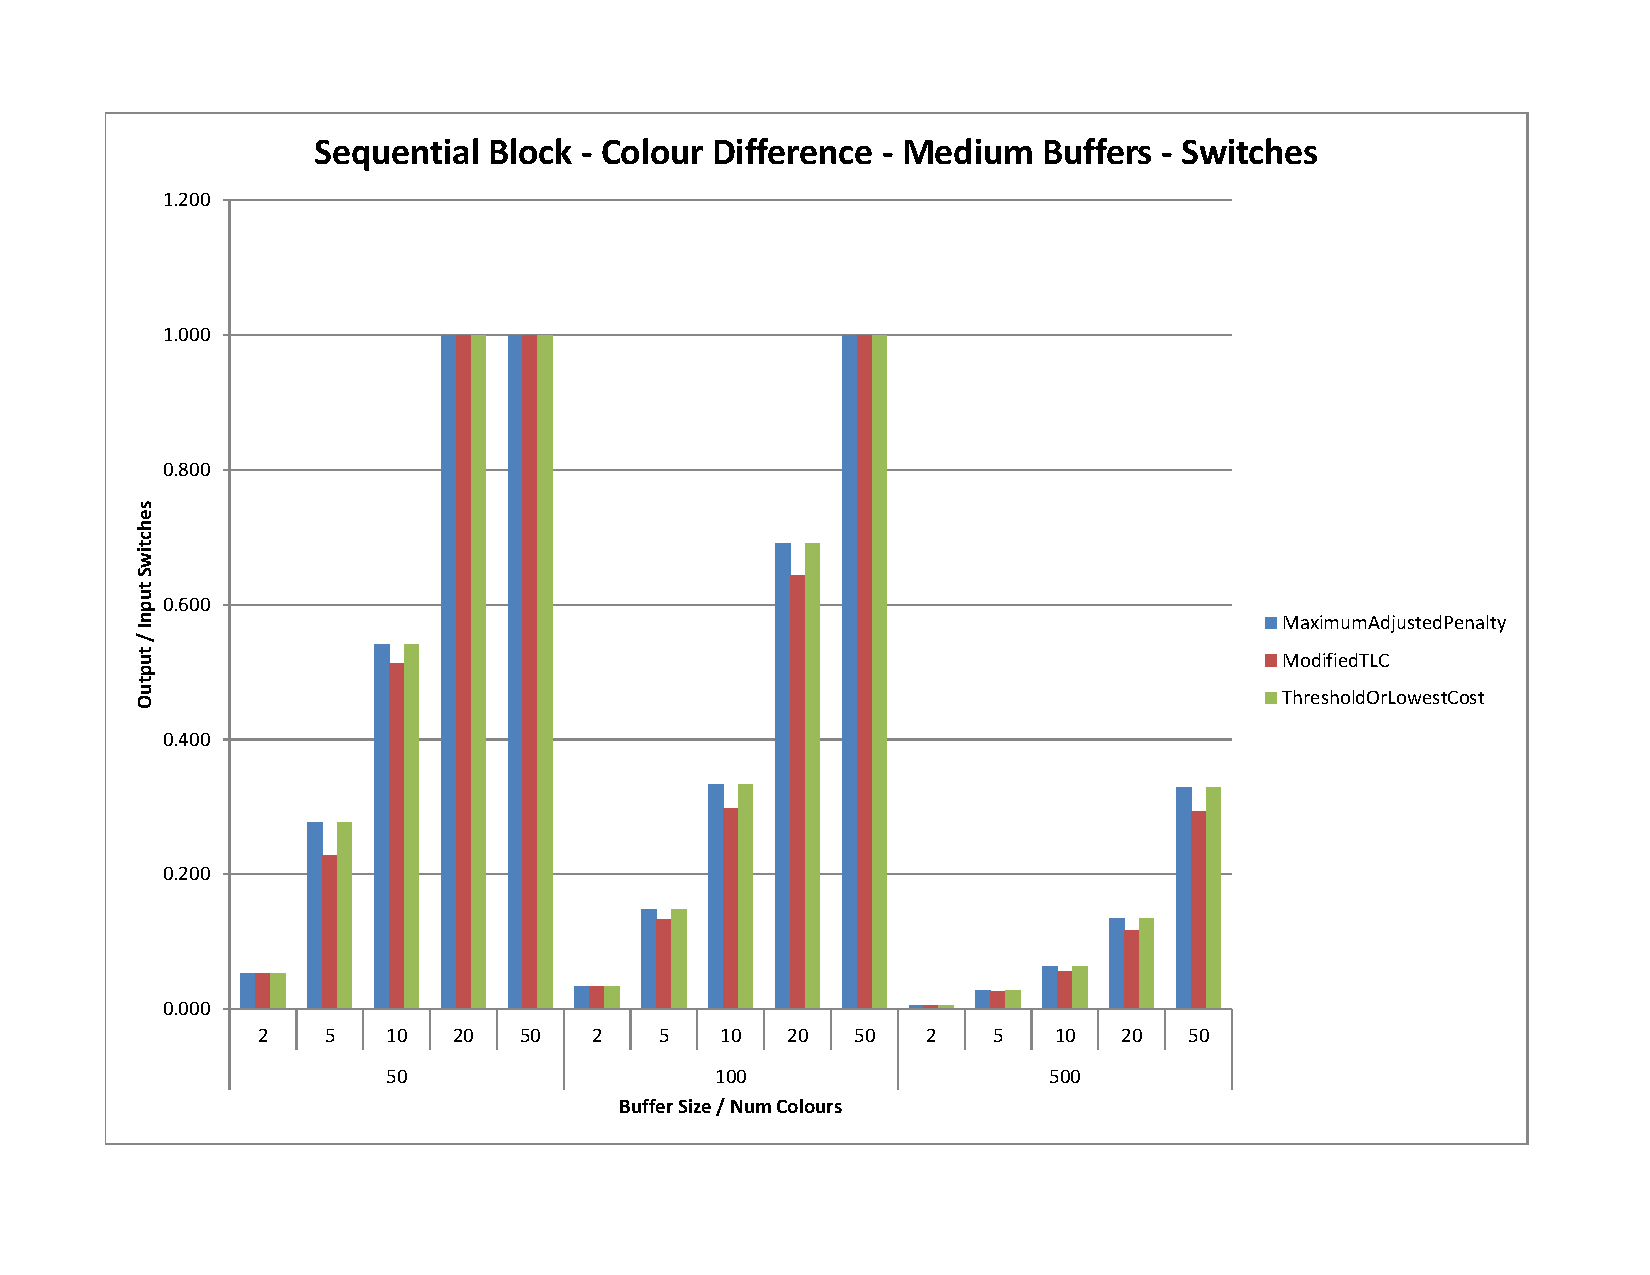
\includegraphics[scale=0.60]{Sequential-Block-cd-medium-switches.pdf}
\caption{TLC' has better switch ratio}
\label{sequentialBlockCDMediumSwitches}
\end{figure}   

For the Uniform cost function, all our algorithms have almost identical switch and cost ratios indicating that they all achieve almost identical reordering. 

\subsection{Comparing TLC and TLC' for Large Data}

In this section we present the experimental results for TLC and TLC' for large data sets. For these experiments, out input sequence size was 1000000, out buffer sizes were 1000, 2000, 5000 and 10000 and the number of colour combinations were 100, 500 and 1000. Since our algorithm uses the same logic as TLC, we have used TLC as the base to compare all our experiments. 

Owing to large size of the data sets, we have restricted our random sequences and random cost functions to 30 times and averaged the restults over these times, unlike the small data sets were we have 100 runs. 

The following subsections present the results observed for each input sequence with different buffers and number of colours combinations. 

\subsubsection{Alternation Sequences}

For Alternation sequences with the Cost Equals Colour cost function, we observe that TLC' has a significantly better switch and cost ratio across all buffer size and number of colours combinations. This result is observed regardless of any inequality for the buffer sizes and number of colours. TLC' has the best reordering ratios when the number of colours are much smaller than the buffer size, but it still has a better performance than TLC when the number of colours are the same as the buffer size. This result is illustrated in Fig. \ref{alternationCCLargeCost}.

\begin{figure}[ht]
\centering 
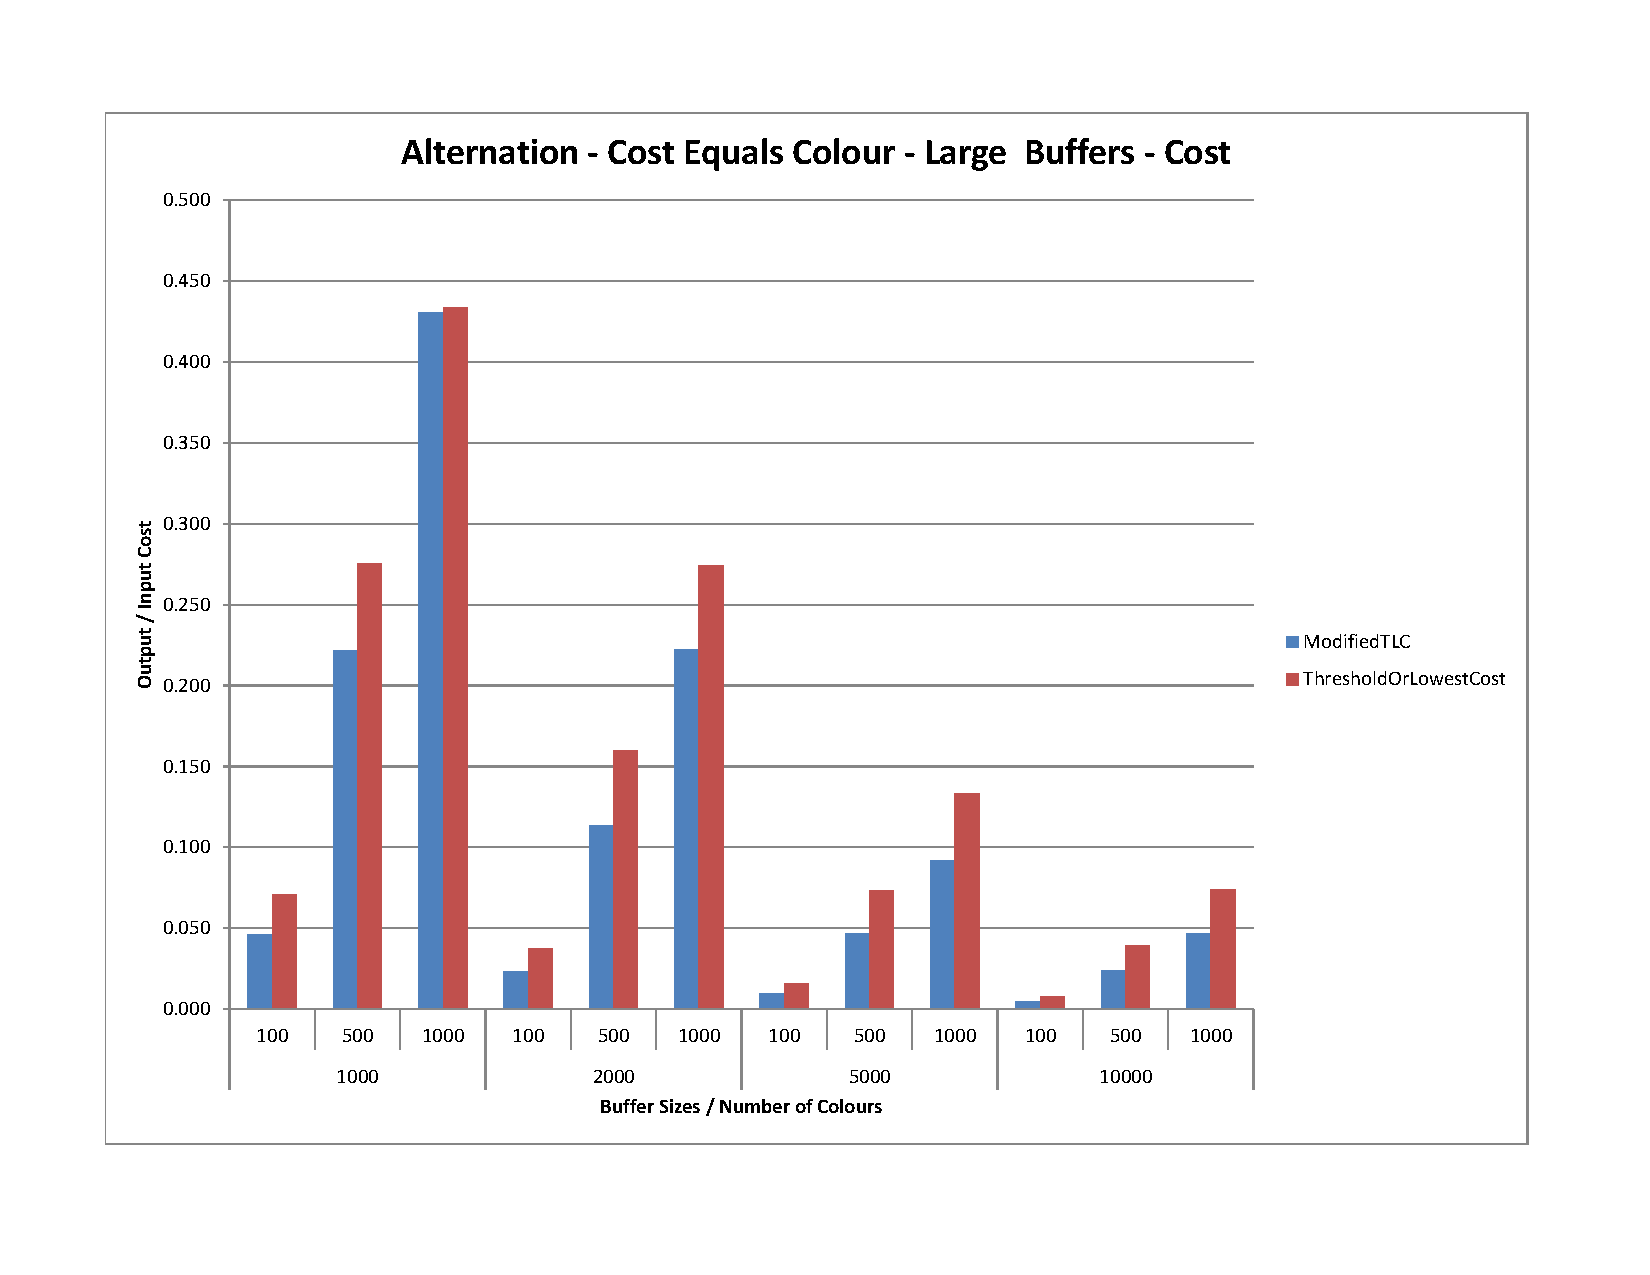
\includegraphics[scale=0.60]{Alternation-cc-large-cost.pdf}
\caption{TLC' has better cost ratio}
\label{alternationCCLargeCost}
\end{figure}   

When comparing switch ratios for the Cost Equals Quadratic Colour cost function, we observe that TLC' has a significantly better switch ratio across all buffer sizes and number of colours. Like with the Cost Equals Colour cost function, out best results are obtained when the number of colours is one-tenth of the buffer sizes. Overall, we still observe very good switch ratios for TLC' when compared to TLC. When it comes to comparing costs, we observe that TLC' has a better cost ratio when the buffer size is at least two times the number of colours ($ k\geq 2 \times C$). 

Our observations for Random cost are inline with the observations for Cost Equals Quadratic Colour cost function where we find that TLC' has a significantly better switch ratio across all buffer size and number of colour combinations and the cost ratio for TLC' is better when the buffer size is at least two times the number of colours. 

Staying consistent with the other cost functions, we observe that TLC' has a significantly better switch ratio for all buffer size and number of colours combinations for the Colour Difference cost function as well. However, as seen in the small data set results, TLC' fails to achieve a good performance when the cost ratios are compared for this cost function. 

Both our algorithms have almost identical switch and cost ratios across all combinations of buffer sizes and number of colours. 

\subsubsection{Delta Sequences}

Like with Alternation Sequences, we observe that TLC' has a better switch ratio than TLC for all buffer sizes for the Cost Equals Colour cost function. Likewise, this result also holds when comparing the cost ratios as we find that the cost ratios for TLC' are better than that for TLC across all buffers. 

Similar observations hold good for the Cost Equals Quadratic Colour cost function where we observe that TLC' has significantly better switch ratios than TLC. This result is illustrated in Fig. \ref{deltaCQLargeSwitches}. TLC' also has a better cost ratio than TLC for this cost function, but the difference is not as significant as that observed with comparing switch ratios. 

\begin{figure}[ht]
\centering 
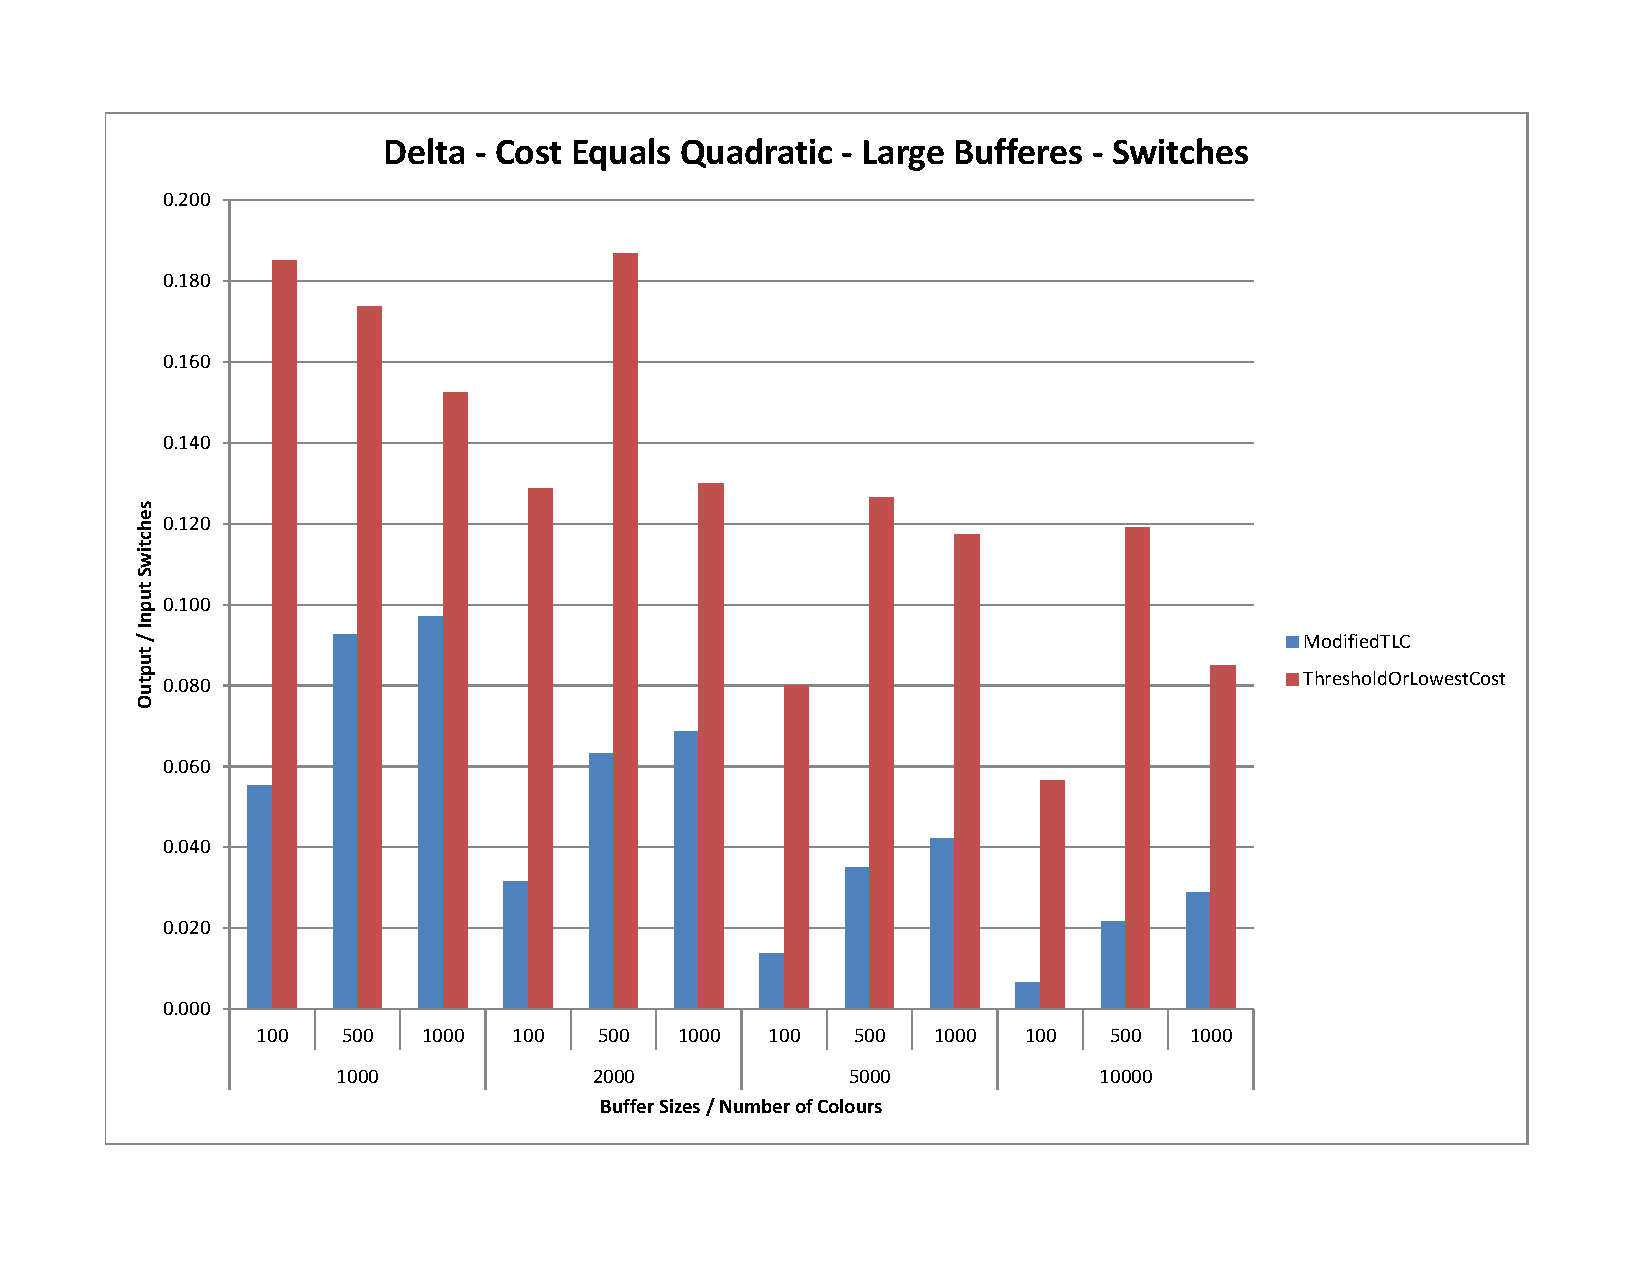
\includegraphics[scale=0.60]{Delta-cq-large-switches.pdf}
\caption{TLC' has a significantly better switch ratio}
\label{deltaCQLargeSwitches}
\end{figure}   

As seen in the previous two cost functions, TLC' has a better switch and cost ratio than TLC even for the Random cost function. Also, like in the previous two cases, it is to be noted that although TLC' has a better cost ratio, our best performance is the switch ratio where TLC' has exceptionally low switches in the output sequence. 

As seen with Alternation Sequences, TLC' has a better switch ratio than TLC for the Colour Difference cost function, however, the cost ratios are significantly higher than TLC. It is to be noted that both algorithms achieve a very good reordering, but TLC has an exceptionally low cost making it the choice of algorithm for this cost function.

For Delta sequences with a Uniform cost function, we observe that TLC' has a slightly worse performance than TLC, which is different from the results we have from the small data sets where both algorithms had almost identical performance for Uniform costs. 

\subsubsection{Random Sequences}

For the Cost Equals Colour cost function, we observe that TLC' has a  better switch and cost ratio than TLC for all buffer sizes and number of colours. Our best results are when the buffer size is much larger than the number of colours, in these cases, we achieve a switch ratios which are very small indicating that the output sequences have very few of the switches originally present in the input sequence. 

We have the exact same observations when we compare the switch and cost ratios for the Cost Equals Quadratic Colour cost funtion. As in the previous case, we observe that TLC' has a significantly lower switch ratio across all combinations of buffer sizes tested. Likewise, TLC' has a lower cost ratio when the cost ratios of TLC and TLC' are compared regardless of the buffer sizes and number of colours. 

For the Random cost, we observe that TLC' has a significantly better  switch ratio regardless of the buffer sizes and number of colours. But when comparing cost ratios, we observe that TLC' has a better significant ratios only when the buffer size is strictly greater than the number of colours, that is $k >= 2 \times C$.

As seen with the other cost functions, we observe that TLC' has a better switch ratio for all combinations of buffers and colours. When comparing costs, both out algorithms do very well with the cost ratios being well below 4\% in the worst case indicating that about 96\% of the switches present in the input sequence were eliminated. However, TLC' has a poor performance compared to TLC as the cost ratios for TLC are all below 0.5\% indicating that the output sequence basically has almost no switches. This is illustrated in Fig. \ref{randomCDLargeCost}.

\begin{figure}[ht]
\centering 
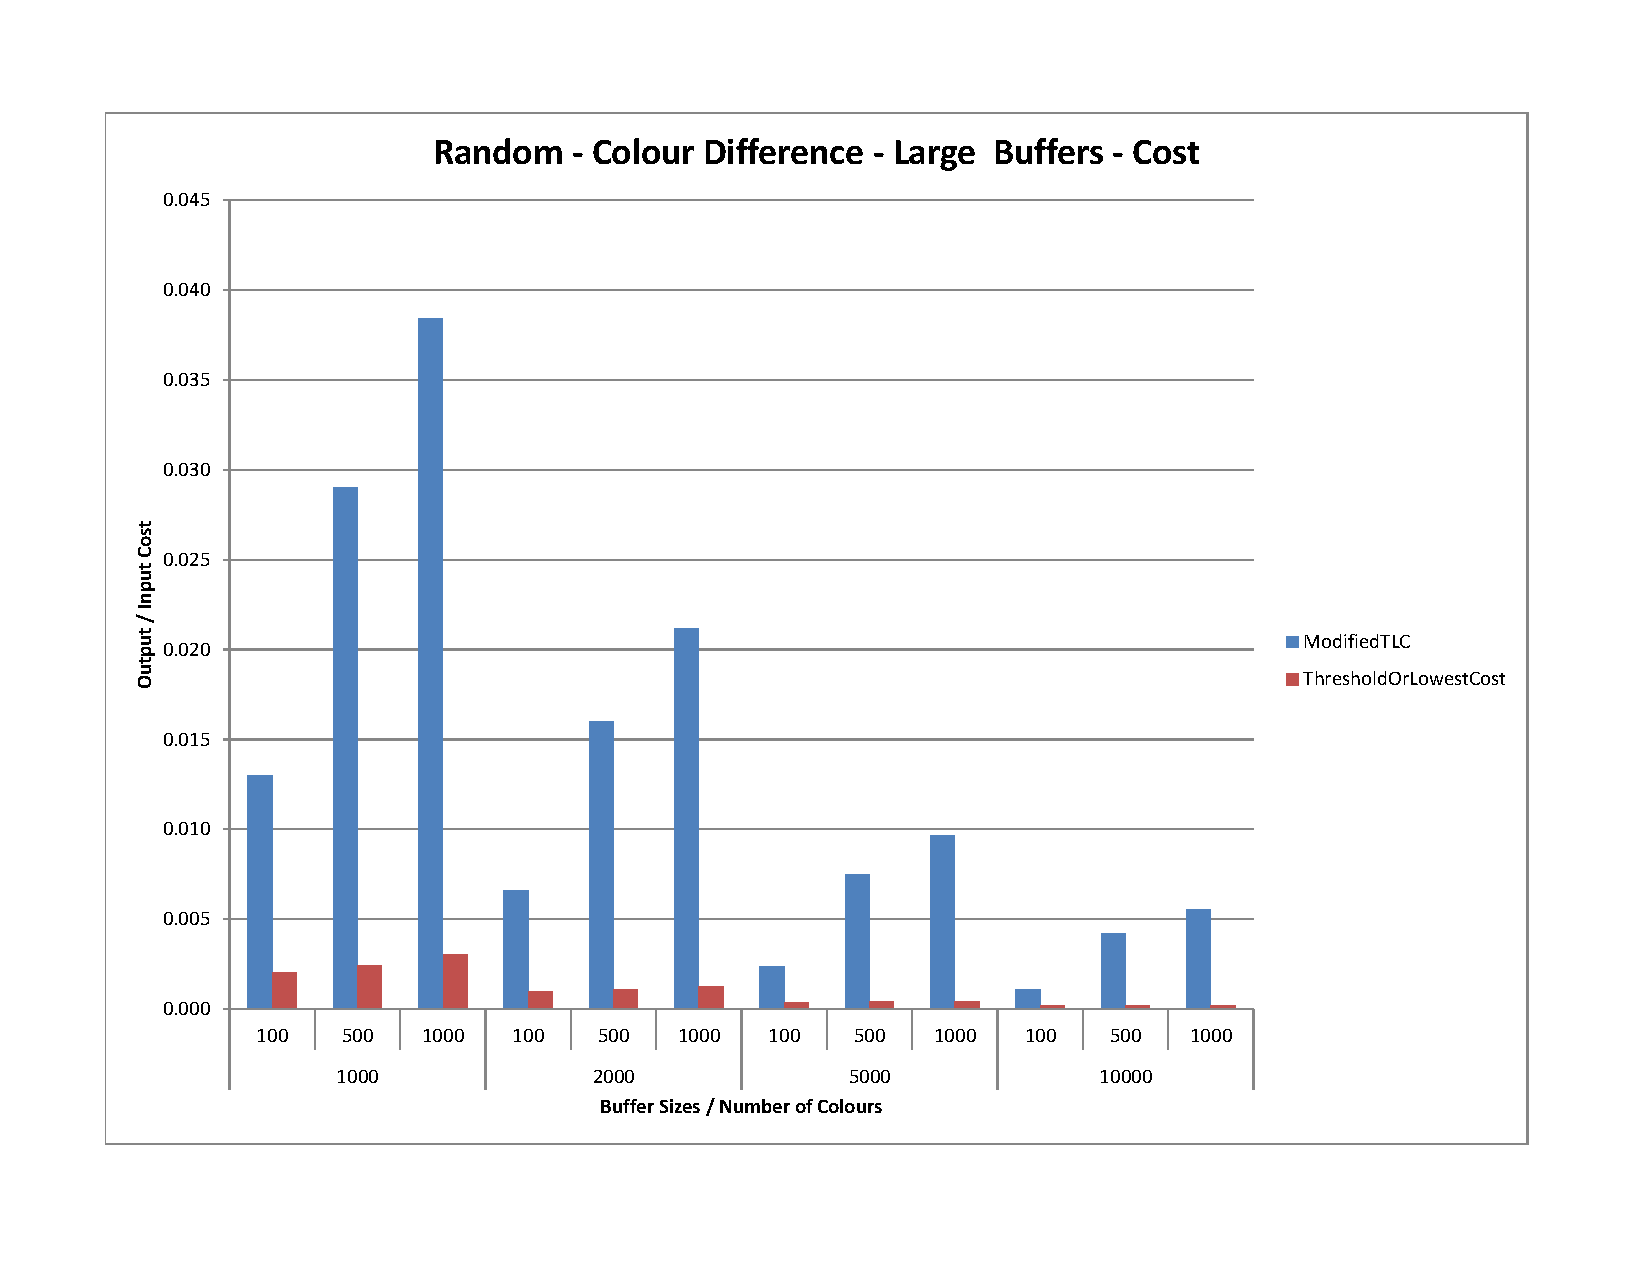
\includegraphics[scale=0.60]{Random-cd-large-cost.pdf}
\caption{TLC performs exceptionally well}
\label{randomCDLargeCost}
\end{figure}   

For Uniform costs, we observe that TLC' has a marginally worse performance when the buffer size is small. Putting in other words, TLC' can achiever a better performance than TLC only when the buffer size is at least two times the number of colours. 

\subsubsection{Random Block Sequences}

When we compare the switch ratio for TLC and TLC' for the Cost Equals Colour cost function, we observe that TLC' has a significantly better switch ratio than TLC, when the number of colours is a fraction of the buffer size. For example, when the buffer size is 10 times the number of colours ($ k = 10 \times C$), we observe that TLC' has 82\% of the switches in the input sequence where as TLC has about 88\% of switches in the input sequence. This is not a very significant difference, but when we compare the switch ratio for these two algorithms when the buffer size is a 100 times the number of colours ($ k = 100 \times C$), we see a significant difference in the switch ratios. In this case, TLC' has 23.5\% of the switches present in the input sequence while TLC has 47.4\% of the original switches. This is a significant result. However, when we compare the cost ratios for these two algorithms, we observe that TLC' only does slightly better than TLC in most cases, the best result being, for buffer size 10000 and 100 colours, TLC' has 23.5\% of the original switches where as TLC has 30.1\%. 

We observe a similar trend when comparing the switch ratios for the Cost Equals Quadratic Colour cost function, where the switch ratio for TLC' gradually decreases as the size of the buffer increases, and it gets to around 50\% of the switch ratio for TLC when the buffer size is significantly large as illustrated in Fig. \ref{randomBlockCQLargeSwitches}. When comparing cost ratios, we observe that as the number of colours increases, TLC' performs marginally worse than TLC across all buffer sizes. Also, for 100 colours, we observe that TLC performs slightly better than TLC' for buffer sizes 1000 and 2000, where as TLC' performs slightly better than TLC for the other two buffer sizes (5000 and 10000). This indicates that TLC' is better suited for larger buffer sizes.

\begin{figure}[ht]
\centering 
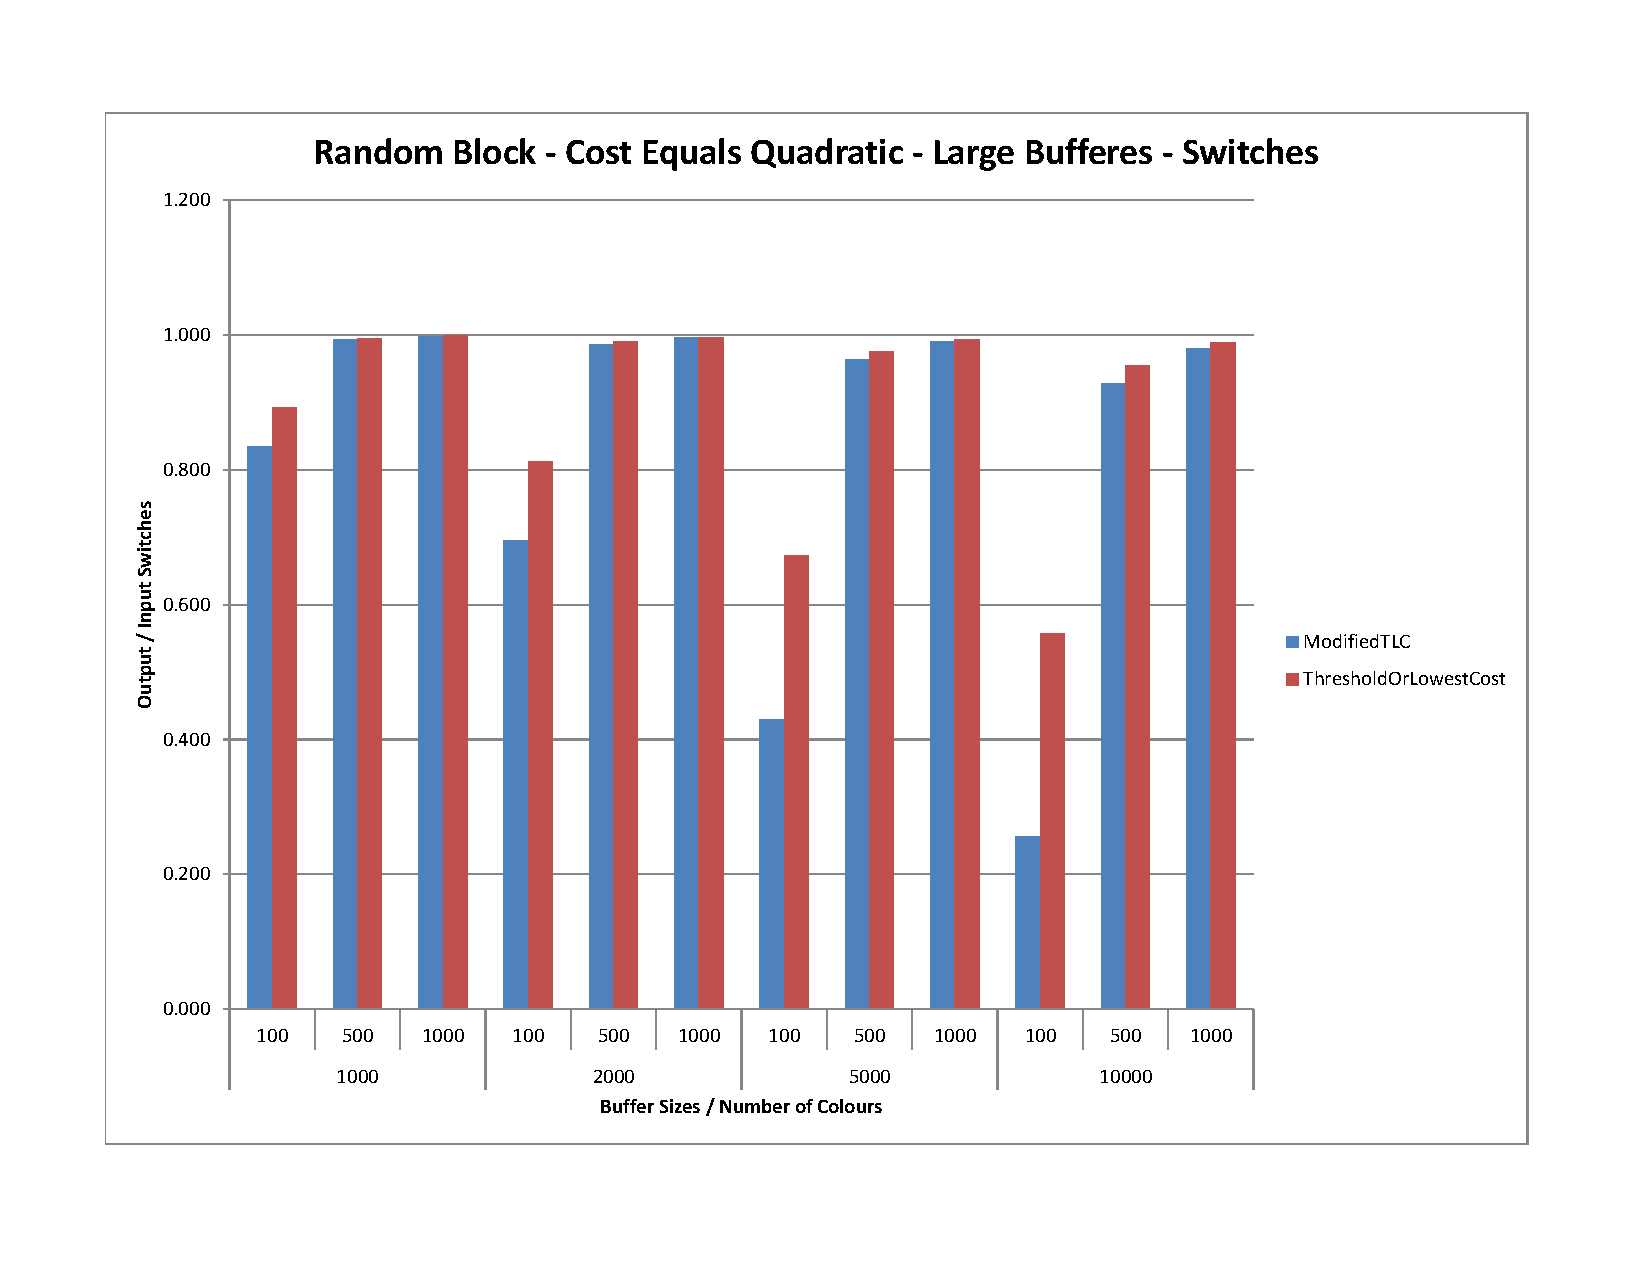
\includegraphics[scale=0.60]{Random-Block-cq-large-switches.pdf}
\caption{TLC' has a significantly better switch ratio}
\label{randomBlockCQLargeSwitches}
\end{figure}   

As in the previous two cost functions, we observe that TLC' achieves a better switch ratio for 100 colours across all buffer sizes. However, we also observe that while the switch ratio was always better for TLC', for the Random cost function, the switch ratio marginally increases for TLC' when the number of colours increases. This behaviour is consistent with all buffer sizes. As to cost ratio comparison, we observe that TLC' has a slightly higher cost ratio across all buffer size and number of colours combinations making TLC the better suited algorithm for this scenario. 

For the Colour Difference cost function, we observe that the switch ratio is slightly better for 100 colours and as the number of colours increases, both have almost identical performance. But when cost ratios are compared, TLC outperforms TLC' by a very large margin as the cost ratio for TLC' for this cost function is very high compared to TLC. 

Both TLC and TLC' have almost identical switch and cost ratios for the uniform cost function making either of them suitable for these scenarios. 

\subsubsection{Sequential Block Sequences}

For the Cost Equals Colour cost function, we observe that TLC' has a better switct ratio than TLC when the buffer size is at least 5 times the number of colours ($ k = 5 \times C$). For other cases, we observe that TLC has a better switch ratio than TLC'. A similar result is obtained when we compare the cost ratios of the two algorithms, in this case we observe that TLC' has a better cost ratio than TLC when the buffer size is at least 10 times the number of colours ($k = 10 \times C$). For all other cases TLC does better than TLC'. 

We see a similar trend with the Cost Equals Quadratic Colour cost function where TLC' has a significantly better switch ratio than TLC when the buffer size is 5 times the number of colours ($k = 5 \times C$).However, when we compare the cost ratios we observe that unlike the Cost Equals Colour cost function, TLC' has a better cost ratio than TLC when the buffer size is at least 5 times the number of colours ($k >= 5 \times C$). This is the same inequality as observed for the switch ratios. 

Our observations for the Random cost function are inline with those for the Cost Equals Colour cost function. We find that Random cost has the exact same inequalities for buffer sizes and number of colours for which TLC' achieves a better performance than TLC, which is $k \geq 10 \times C$ for switches and $k \geq 5 \times C$ for costs. This result is presented in Fig. \ref{sequentialBlockRCLargeCost}.

\begin{figure}[ht]
\centering 
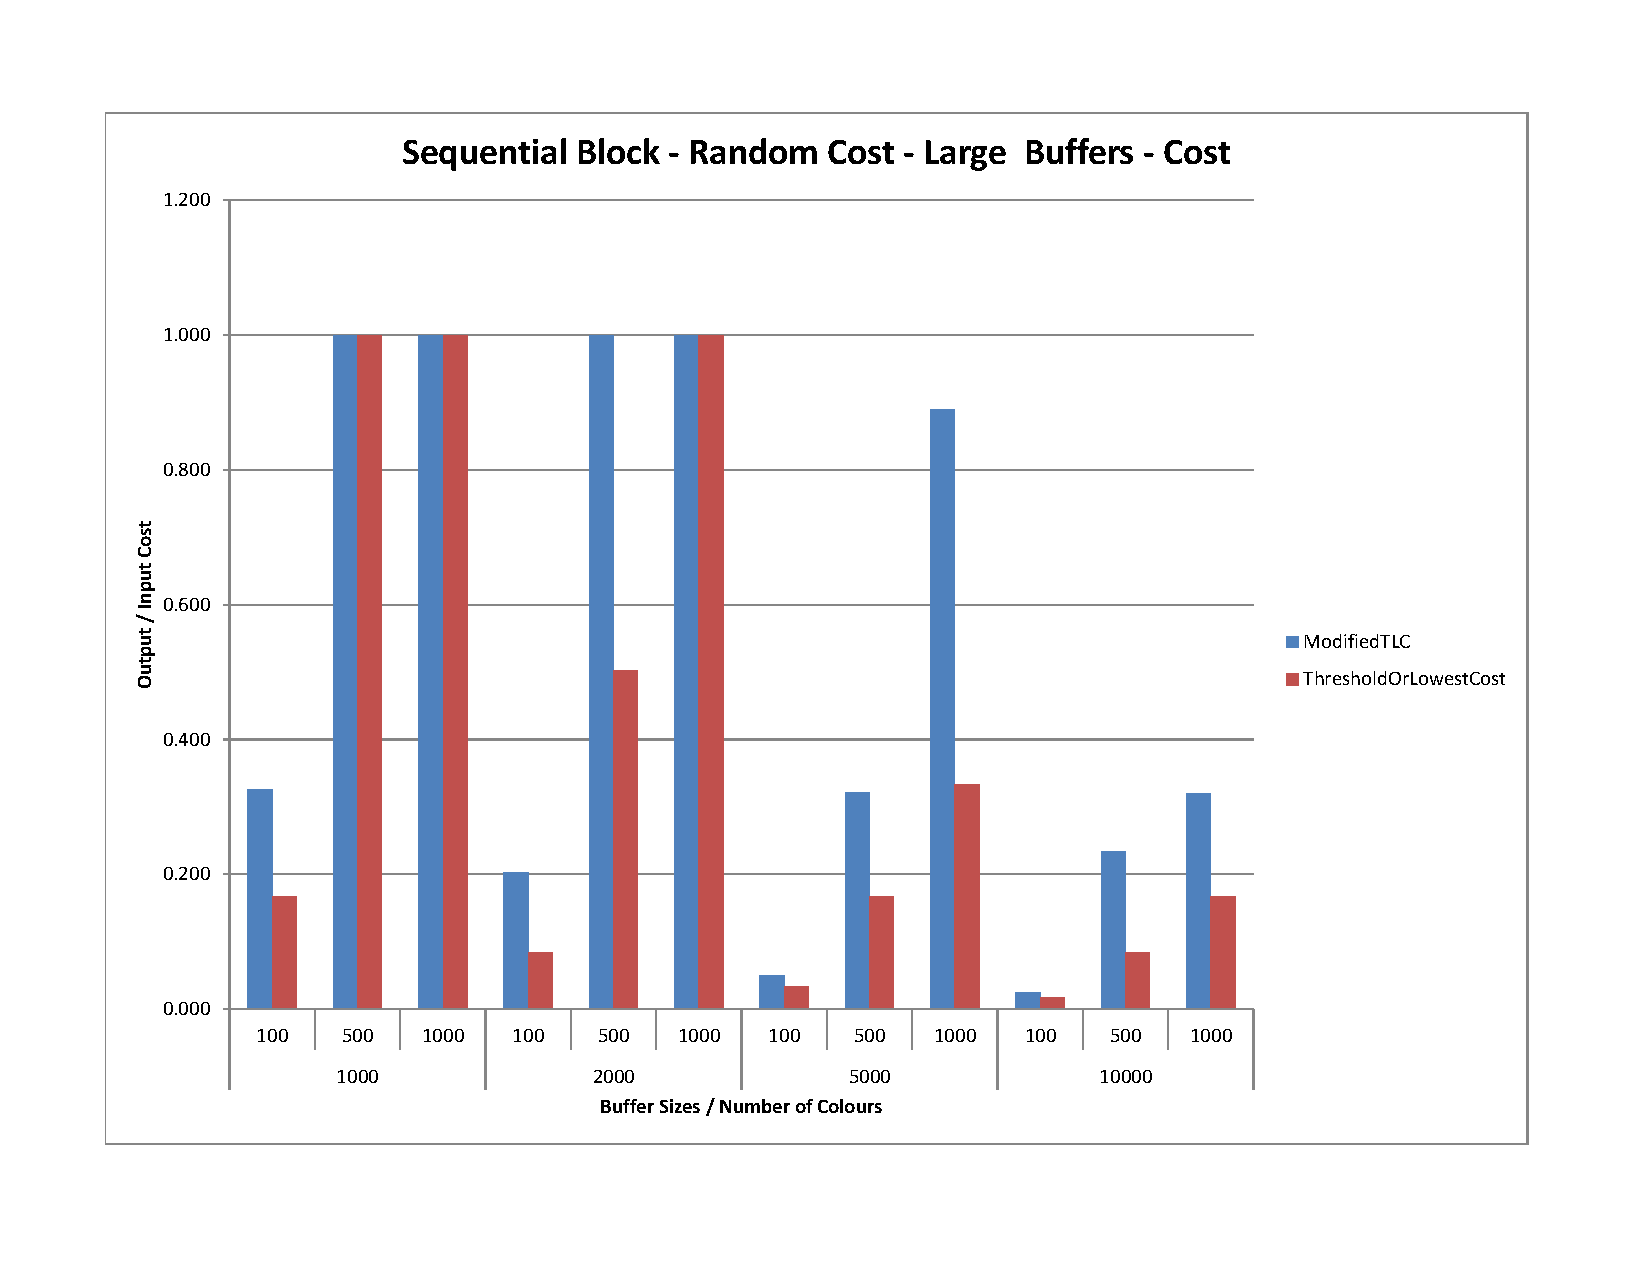
\includegraphics[scale=0.60]{Sequential-Block-rc-large-cost.pdf}
\caption{TLC' has a significantly better switch ratio when $k \geq 5 \times C$}
\label{sequentialBlockRCLargeCost}
\end{figure}   

The switch ratio for the Colour Difference cost function follows the same inequality as the switch ratio for the other cost functions, where TLC' has a better switch ratio than TLC when the buffer size is at least 5 times the number of colours. But when comparing cost ratios we observe that TLC' does not have a good performance across all buffer size and number of colours combinations. This is inline with the results obtained for other cost functions. 

As seen with the other input sequence types, both TLC and TLC' have almost identical performance when the cost is Uniform. 

